%% ===============================================================
%% main.tex -- The Main Document File
%% ===============================================================

\documentclass[acmsmall]{acmart}

% --- 1. PREAMBLE: Load all packages and custom commands ---
%% ===============================================================
%% preamble.tex -- Preamble for packages and global settings
%% ===============================================================

% The \BibTeX command to typeset BibTeX logo
\AtBeginDocument{%
  \providecommand\BibTeX{{%
    Bib\TeX}}}

% --- Packages ---
\usepackage{graphicx}
\usepackage{natbib}
% \usepackage{amsmath}
% \usepackage{booktabs}
% \usepackage{hyperref}
% \usepackage{cleveref}
\usepackage{geometry}
\usepackage{tikz}
\usetikzlibrary{
    shapes.geometric, % for shapes such as rectangles
    arrows.meta,      % for arrow styles
    positioning,      % for node positioning (e.g., right=of)
    calc              % for coordinate calculation
}


\usepackage{booktabs}
\usepackage{multirow}
\usepackage{makecell}
\usepackage{pifont}

% --- Define styles used in the diagrams ---
\tikzset{
    main/.style = {rectangle, rounded corners, draw=black, thick, fill=blue!10, text width=2.8cm, minimum height=0.7cm, align=center, font=\small},
    sub/.style = {rectangle, rounded corners, draw=black, thick, fill=blue!5, text width=3cm, minimum height=0.6cm, align=center, font=\small},
    leaf/.style = {rectangle, draw=black, thick, fill=gray!5, text width=10cm, align=left, font=\footnotesize},
    line/.style = {thick} 
}


\usepackage[edges]{forest}
\usepackage{etoolbox}
\robustify\citep



% --- Tighten figure/table spacing globally ---
\setlength{\intextsep}{6pt plus 2pt minus 2pt}      % was ~12pt
\setlength{\floatsep}{8pt plus 2pt minus 2pt}        % was ~12pt
\setlength{\textfloatsep}{8pt plus 2pt minus 2pt}    % was ~20pt
\setlength{\abovecaptionskip}{4pt}                    % was ~10pt
\setlength{\belowcaptionskip}{0pt}                    % was ~0pt

% Tells LaTeX to look for images in the 'figures/' folder
\graphicspath{{figures/}}




% --- 2. METADATA: Rights, Conference, Title, Authors, etc. ---
% Replace with your actual rights information
\acmJournal{CSUR}
\setcopyright{acmlicensed}
\copyrightyear{2025}
\acmYear{2025}
\acmDOI{XXXXXXX.XXXXXXX}


\newcommand{\yuji}[1]{\textcolor{red}{Yuji: #1}}


\title{Inference-Time Control for Trustworthy Large Language Models: A Survey}

\author{Yuyang Bai}
\authornote{Project Leader.}
\authornote{Major Contributor.}
\affiliation{%
  \institution{Texas A\&M University}
  \country{USA}
}
\email{ybai@tamu.edu}

\author{Zheyuan Liu}
\authornotemark[1]
\authornotemark[2]
\affiliation{%
  \institution{University of Notre Dame}
  \country{USA}
}
\email{zliu29@nd.edu}

\author{Han Yan}
\authornotemark[2]
\affiliation{%
  \institution{University of Notre Dame}
  \country{USA}
}
\email{yanh8284@gmail.com}

\author{Zhangchen Xu}
\authornotemark[2]
\affiliation{%
  \institution{University of Washington}
  \country{USA}
}
\email{zxu9@uw.edu}

\author{Yixin Wan}
\authornotemark[2]
\affiliation{%
  \institution{University of California, Los Angeles}
  \country{USA}
}
\email{elaine1wan@cs.ucla.edu}

\author{Canyu Chen}
\authornotemark[2]
\affiliation{%
  \institution{Northwestern University}
  \country{USA}
}
\email{canyuchen@u.northwestern.edu}

\author{Zehong Wang}
\authornotemark[2]
\affiliation{%
  \institution{University of Notre Dame}
  \country{USA}
}
\email{zwang43@nd.edu}

\author{Xiangchi Yuan}
\authornotemark[2]
\affiliation{%
  \institution{Georgia Institute of Technology}
  \country{USA}
}
\email{xyuan300@gatech.edu}

\author{Yue Huang}
\authornotemark[2]
\affiliation{%
  \institution{University of Notre Dame}
  \country{USA}
}
\email{yhuang37@nd.edu}

\author{Guangyao Dou}
\authornotemark[2]
\affiliation{%
  \institution{Johns Hopkins University}
  \country{USA}
}
\email{gdou1@jhu.edu}

\author{Yuji Zhang}
% \authornotemark[2]
\affiliation{%
  \institution{University of Illinois at Urbana-Champaign}
  \country{USA}
}
\email{yujiz@illinois.edu}

\author{Zhuofeng Li}
% \authornotemark[2]
\affiliation{%
  \institution{Texas A\&M University}
  \country{USA}
}
\email{zhuofengli@tamu.edu}

\author{Hangxiao Zhu}
% \authornotemark[2]
\affiliation{%
  \institution{Texas A\&M University}
  \country{USA}
}
\email{hangxiao@tamu.edu}

\author{Xiangliang Zhang}
\affiliation{%
  \institution{University of Notre Dame}
  \country{USA}
}
\email{xzhang33@nd.edu}


\author{Yu Zhang}
\authornote{Corresponding Author.}
\affiliation{%
  \institution{Texas A\&M University}
  \country{USA}
}
\email{yuzhang@tamu.edu}

\author{Meng Jiang}
\authornotemark[3]
\affiliation{%
  \institution{University of Notre Dame}
  \country{USA}
}
\email{mjiang2@nd.edu}

% A short version of authors for page headers
\renewcommand{\shortauthors}{Bai et al.}
\newcommand{\cmark}{\textcolor{green!50!black}{\ding{51}}}
\newcommand{\xmark}{\textcolor{red!70!black}{\ding{55}}}

% --- CCS and Keywords ---
\begin{CCSXML}
<ccs2012>
   <concept>
       <concept_id>10002978.10003029</concept_id>
       <concept_desc>Security and privacy~Human and societal aspects of security and privacy</concept_desc>
       <concept_significance>500</concept_significance>
       </concept>
 </ccs2012>
\end{CCSXML}

\ccsdesc[500]{Security and privacy~Human and societal aspects of security and privacy}
\keywords{Large Language Models, Trustworthy AI, Inference-Time Control}

% --- 3. DOCUMENT BODY ---
\begin{document}


%% chapters/00-abstract.tex
\begin{abstract}
 \yuji{Title: Inference-time harnessing?} Inference-time methods are becoming an important tool for improving the trustworthiness of large language models after deployment. Unlike training-time alignment, which is often costly or difficult to revise once a model is released, inference-time interventions can adapt model behavior under changing requirements without retraining. This survey presents a unified review of inference-time trustworthiness methods across safety, privacy, fairness, and factuality. We organize the field using a pipeline-grounded taxonomy with three tiers: External Controls, Internal Manipulations, and System-Level Orchestration. Through this framework, we summarize major methods, analyze their trade-offs, and discuss open challenges and future directions for reliable deployment-time control.
\end{abstract}

\maketitle

% --- Introduction ---
\section{Introduction}
\label{sec:intro}
% \textcolor{red}{TODO: (1) Survey Comparison table (with other surveys and perspectives.) (2) Modify the intro and structures (3) keep refining the figures}

\begin{figure*}[htbp]
  \centering
  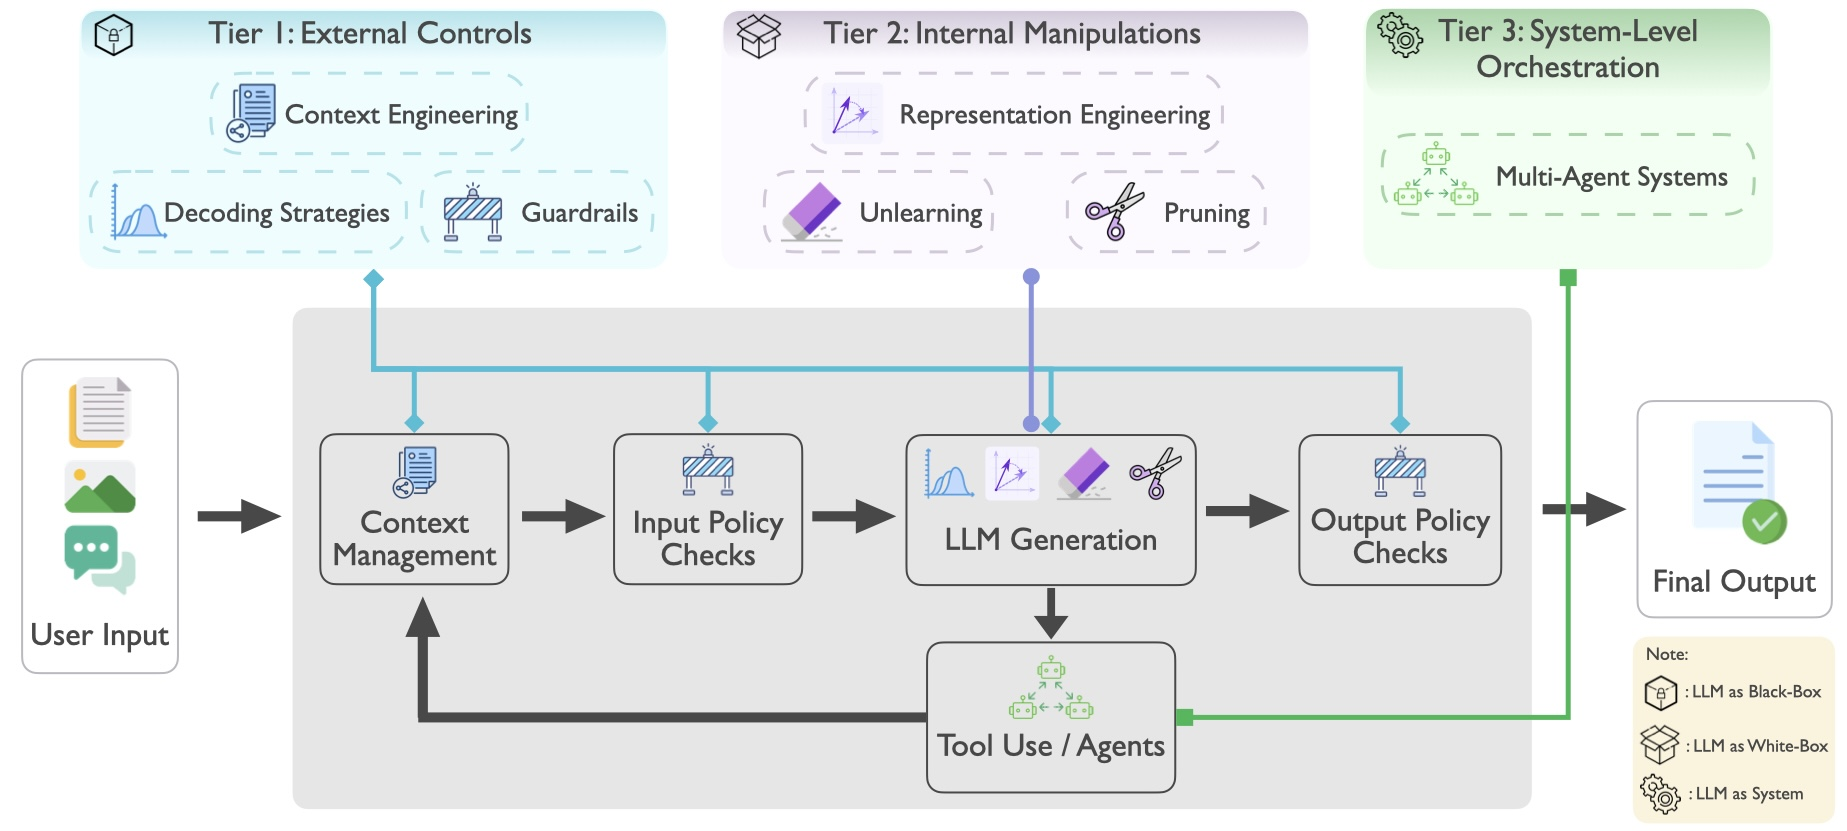
\includegraphics[width=1\linewidth]{figures/intro_v2.jpeg}
  \caption{Taxonomy (top) and attachment points in an inference-time pipeline (bottom). We organize seven inference-time methods into three tiers---\emph{External Controls} (Context Engineering, Guardrails, Decoding Strategies), \emph{Internal Manipulations} (Representation Engineering, Unlearning, Pruning), and \emph{System-Level Orchestration} (Multi-Agent Systems)---and map each to its point of intervention in the generation pipeline.}
  \label{fig:taxonomy_pipeline}
\end{figure*}

% Large Language Models (LLMs) and Multimodal Large Language Models (MLLMs) have rapidly moved from research prototypes to deployed systems in domains such as healthcare, law, and finance. Models are now accessed primarily through APIs, regulatory frameworks like the EU AI Act are imposing new behavioral requirements, and new vulnerabilities are discovered continuously after deployment. These pressures expose a fundamental limitation of training-time alignment alone. Once a model is released, updating its behavior is often slow, costly, or simply impossible for downstream users. In this survey, we study trustworthiness as the ability to maintain safe, fair, privacy-preserving, and reliable behavior at deployment time, and we argue that inference-time mechanisms are not merely a complement to training-time alignment but an increasingly necessary layer of control in their own right.

% \textcolor{red}{(1) Core Principles, shorten.
% (2) Applications, each trustworthy perspective has one paragraph (maybe delete some citations)
% (3) Move all of the discussion sections to the end (later sections can be divided by the methods)}

\textcolor{red}{Next step: 
\begin{enumerate}
    \item Figure 1, Figure 6 (misunderstanding), Figure 4 (font, size), Table 1 (larger font)
    \item for each figure, larger font (like figure 8)
\end{enumerate}
}

% \textcolor{red}{Yuyang: 
% \begin{enumerate}
%     \item Shorten/merge discussion part (2 page and a half -> 1 page and a half or 2 pages).
%     \item Remove some citations (Do so by updating the taxonomy), I would say shorten it to around 200 citations (now 240+). Just try your best first, I will help you later if this can't be done. 
%     \item Add name lists. The first three authors: Yuyang (Project leaders), Zheyuan (Project leaders), Han, .... (Other students are major contributors). Example below:
% \end{enumerate}
% }

% \textcolor{blue}{Han: (1) Redraw Figure 6 (Decoding pipeline)
% (2) Help modifying paper after adviser's review}

% \textcolor{cyan}{Logistic:
% \begin{enumerate}
%     \item Do we need taxonomy tree?
%     \item Let Meng, Yu review first before we invite other collaborators.
%     \item Recheck the format, CCS concepts keywords, additional key words and template (low priority)
%     \item Invitation List: Mohit, kaiwei, nanyun, Manling, Jieyu, Xiangliang, Heng (low priority)
%     \item Create a repo to hold all papers.
% \end{enumerate}
% }
\yuji{consider talking more about trustworthiness in high-stakes domains since the community starts to believe general reasoning has high reliability... Also connect the motivation to the recently more popular concept of ``harnessing''}
Large Language Models (LLMs) and Multimodal Large Language Models (MLLMs) have rapidly moved from research prototypes to deployed systems in domains such as healthcare, law, and finance. Models are now accessed primarily through APIs, regulatory frameworks like the EU AI Act are imposing new behavioral requirements, and new vulnerabilities are discovered continuously after deployment. Existing survey has largely emphasized train-time trustworthiness, where safety, fairness, privacy, or factuality objectives are encoded during parameter learning through data curation, supervised alignment, or preference optimization. These methods aim to shape the model’s default behavior globally and persistently by modifying what the model internalizes.

In this survey, we distinguish this perspective from inference-time trustworthiness, which concerns mechanisms that regulate model behavior at runtime after training has been completed. Rather than changing the model’s learned parameters alone, inference-time methods operate on the generation process through contextual control, decoding-time intervention, representation engineering, internal steering, or multi-agent verification. This distinction extends beyond considerations of efficiency or convenience. More fundamentally, train-time and inference-time methods differ in where control is exercised, how persistent the intervention is, and what level of guarantees it can provide. Train-time methods primarily shape a model’s behavioral prior, whereas inference-time methods determine how that prior is enacted, constrained, or corrected in a specific interaction context.

These two forms of trustworthiness are complementary. Train-time alignment is well suited for establishing broad and stable default behavior, but deployment introduces context-specific risks that cannot always be fully included during training, including changing policies, user-specific constraints, retrieval contamination, adversarial prompting, and jurisdiction-dependent requirements. Inference-time mechanisms provide a second control plane that is local, adaptive, and often more directly auditable at the level of individual interactions. They offer a complementary control layer that can steer, constrain, or monitor model behavior after deployment. Because they are often lightweight and modular, they are well suited to dynamic and context-specific trustworthiness requirements. Conversely, inference-time control alone cannot substitute for robust underlying models, because runtime interventions may be brittle, reactive, or incomplete without strong train-time foundations.\yuji{The two sentences sound like strong claims. Maybe consider supporting the two claims with abandant evidence (references)} A full account of trustworthy LLM deployment therefore requires treating trustworthiness as a multi-layer property spanning both training and inference.


% Training-time alignment methods such as instruction tuning and RLHF are central to shaping the general behavior of language models before deployment. However, once a model is released, updating that behavior is often slow, costly, or impossible, especially when users only have API access or limited control over model weights. This creates a practical gap between static alignment and real-world deployment, where requirements can change quickly. Organizations may need to revise safety policies, adapt behavior across users or jurisdictions, satisfy regulatory demands for transparent filtering or redaction, or respond to newly discovered vulnerabilities and distribution shifts. In these settings, retraining is often too rigid. Inference-time methods offer a complementary control layer that can steer, constrain, or monitor model behavior after deployment. Because they are often lightweight and modular, they are well suited to dynamic and context-specific trustworthiness requirements.

Many inference-time techniques were first developed to improve model performance, such as reducing latency, improving fluency, or grounding outputs through retrieval. More recently, they have also been adapted to support trustworthiness during deployment, including safety, privacy, fairness, and factuality. This shift calls for a more unified view of the field. In this survey, we organize inference-time trustworthiness methods by the mechanism and locus of control they introduce during generation. As shown in Figure~\ref{fig:taxonomy_pipeline}, we group them into three tiers: \textbf{External Controls}, \textbf{Internal Manipulations}, and \textbf{System-Level Orchestration}. This perspective highlights shared design patterns and clarifies trade-offs in granularity, invasiveness, and modularity. These tiers differ in where and how they intervene, ranging from black-box control around the model, to white-box intervention inside the model, to coordinated control across multiple agents.

\paragraph{Tier 1: External Controls.} These methods treat the model as a black box. They shape behavior by modifying the inputs, decoding process, or outputs, without changing internal weights or activations. These methods correspond to the \emph{context assembly}, \emph{input policy checks}, \emph{decoding}, and \emph{output policy checks} stages. This tier includes three categories:

\begin{itemize}
\item \textbf{Context Engineering} (Section~\ref{sec:context_engineering}): Strategic prompt design through rules, instructions, or few-shot exemplars to guide outputs without modifying model parameters.
\item \textbf{Guardrails} (Section~\ref{sec:guardrails}): External modules that inspect inputs or outputs against safety or policy constraints, blocking, redacting, or regenerating content when violations occur.
\item \textbf{Decoding Strategies} (Section~\ref{sec:decoding}): Manipulation of token-level distributions during generation to promote desired attributes or suppress undesired ones.
\end{itemize}

\paragraph{Tier 2: Internal Manipulations} require white-box access to the model. They intervene directly in the model's internal computation, such as by steering activations, removing learned behaviors, or pruning architectural components. In the pipeline, these methods operate within the \emph{LLM generation} stage. This tier includes three categories:

\begin{itemize}
\item \textbf{Representation Engineering} (Section~\ref{sec:representation_engineering}): Direct modification of internal activations by adding or subtracting steering vectors associated with specific concepts.
% \item \textbf{Editing} (Section~\ref{sec:editing}): Localized parameter updates to correct facts, update knowledge, or remove harmful associations efficiently.
\item \textbf{Unlearning} (Section~\ref{sec:unlearning}): Targeted removal of information, behaviors, or biases from a pre-trained model to fulfill data-forgetting requirements or disable harmful capabilities.
\item \textbf{Pruning} (Section~\ref{sec:pruning-core}): Post-training removal of weights, neurons, or attention heads, originally for efficiency but now increasingly explored for trust-related effects.
\end{itemize}

\paragraph{Tier 3: System-Level Orchestration} moves beyond single-model intervention. Rather than steering one model in isolation, this tier coordinates multiple LLM agents through structured interaction patterns such as debate, cross-verification, and role specialization. In the pipeline, the \emph{tool use / agents} loop spans context assembly, generation, and output checking, enabling iterative feedback and self-correction. This tier contains one category:

\begin{itemize}
\item \textbf{Multi-Agent Systems} (Section~\ref{sec:multi_agent_systems}): Coordinated agent interactions such as debate or cross-verification, where reliability is strengthened through collaboration.
\end{itemize}

These three tiers form a defense-in-depth view of inference-time trustworthiness. External controls provide lightweight and modular policy enforcement. Internal manipulations enable more direct and fine-grained behavioral intervention. System-level orchestration introduces an additional layer of reliability through collaborative reasoning and feedback. Across this taxonomy, we focus on four dimensions of trustworthiness: \textbf{Safety}, which concerns preventing harmful, biased, or malicious outputs and defending against misuse such as jailbreaks; \textbf{Privacy}, which concerns limiting training-data leakage and protecting user inputs during inference; \textbf{Fairness}, which concerns reducing systematic disadvantages toward individuals or groups; and \textbf{Factuality}, which concerns grounding model outputs in verifiable knowledge and reducing hallucinations. By synthesizing these developments, this survey aims to provide a unified framework for understanding inference-time trustworthiness methods, their trade-offs, and their opportunities for combination under real-world deployment constraints.

\subsection{Related Surveys}
Our work sits at the intersection of three strands: inference efficiency, post-training capability enhancement, and broad-spectrum trustworthiness.

\paragraph{Efficiency-Focused Surveys.}
Comprehensive surveys review inference-time optimizations such as quantization, distillation, and speculative decoding~\citep{survey:inference_efficiency1}. Others target specialized settings like Mixture-of-Experts~\citep{survey:inference_moe} or memory-footprint reduction for large deployments~\citep{survey:inference_efficiency2}. These studies are foundational for understanding mechanics and cost, but their primary objective is computational performance rather than the explicit control of trustworthy behavior.

\paragraph{Surveys on Post-Training Capability Enhancement.}
A second line examines methods applied after pre-training to improve complex-task performance, including prompting-based techniques and reinforcement learning advances~\citep{survey:post-training1, survey:post-training2}. The focus is to make models more capable reasoners or tool users. Alignment is peripheral; fine-grained enforcement of safety, privacy, or fairness at deployment is not the central goal.

\paragraph{Trustworthy-Focused Surveys.}
Holistic surveys chart the landscape of trustworthy LLMs from data integrity to evaluation~\citep{survey:trustworthy1, survey:trustworthy2}. Other work dives deep into specific facets---mitigating social bias in text-to-image generation~\citep{survey:trustworthy_text2img}, safety for autonomous LLM agents~\citep{survey:trustworthy_agents}, or machine unlearning~\citep{survey:unlearning1, survey:unlearning2}. While invaluable, these efforts either organize by harm type or by a single solution family. To our knowledge, none provides a systematic, unified taxonomy that treats \emph{inference-time methods as a control plane} for trustworthiness across safety, privacy, fairness, and factuality.

\subsection{Contributions and Organization}
This survey analyzes inference-time methods for enhancing the trustworthiness of LLMs. Our primary contribution is a unified, pipeline-grounded taxonomy that organizes post-hoc control techniques into seven categories across three tiers---External Controls (Context Engineering, Guardrails, Decoding Strategies), Internal Manipulations (Representation Engineering, Unlearning, Pruning), and System-Level Orchestration (Multi-Agent Systems)---and evaluates them against four deployment-critical dimensions: Safety, Privacy, Fairness, and Factuality. Our key contributions are as follows:

\begin{itemize}
    \item \textbf{A Pipeline-Grounded, Three-Tier Taxonomy of Inference-Time Methods.} We organize seven categories of inference-time control into a coherent three-tier hierarchy---External Controls, Internal Manipulations, and System-Level Orchestration---grounded in the inference-time pipeline (Figure~\ref{fig:taxonomy_pipeline}). This structure clarifies each method's point of intervention, access requirements, and composability within a defense-in-depth design.
    \item \textbf{Systematic Cross-Dimensional Analysis.} We analyze how each category addresses Safety, Privacy, Fairness, and Factuality, clarifying capabilities, limitations, and trade-offs under deployment constraints.
    \item \textbf{Future Directions and Open Challenges.} We synthesize open problems on scalability, evaluation, and composition, and outline a research agenda for real-world systems.
\end{itemize}

The remainder of the survey is organized as follows. \textbf{Section~\ref{sec:external_controls}} presents the three External Controls---Context Engineering, Guardrails, and Decoding Strategies---that operate on inputs, outputs, or the token-selection process without accessing model internals. \textbf{Section~\ref{sec:internal_manipulations}} covers four Internal Manipulations---Representation Engineering, Unlearning, and Pruning---that intervene on the model's activations or parameters. \textbf{Section~\ref{sec:system_level}} discusses System-Level Orchestration through Multi-Agent Systems. \textbf{Section~\ref{sec:evaluation}} provides a critical analysis of evaluation benchmarks and trade-offs. \textbf{Section~\ref{sec:challenges}} consolidates open challenges and future directions. \textbf{Section~\ref{sec:conclusion}} concludes the survey.


% \begin{table*}[t]
% \centering
% \small
% \setlength{\tabcolsep}{4pt}
% \renewcommand{\arraystretch}{1.2}
% \caption{Comparison with existing surveys on inference-time trustworthiness metrics and methods.}
% \label{tab:survey_comparison}
% \resizebox{\textwidth}{!}{
% \begin{tabular}{l|cccc|cccccccc}
% \toprule
% \multirow{4}{*}{\textbf{Surveys}} 
% & \multicolumn{4}{c}{\textbf{Inference-time Metrics}} 
% & \multicolumn{8}{c}{\textbf{Inference-time Methods}} \\
% \cmidrule(lr){2-5} \cmidrule(lr){6-13}
% & \multicolumn{4}{c}{\textbf{Trustworthiness Dimensions}}
% & \multicolumn{3}{c}{\textbf{External Controls}}
% & \multicolumn{4}{c}{\textbf{Internal Manipulations}}
% & \multicolumn{1}{c}{\textbf{System-Level Orchestration}} \\
% \cmidrule(lr){2-5} \cmidrule(lr){6-8} \cmidrule(lr){9-12} \cmidrule(lr){13-13}
% & \textbf{Safety} 
% & \textbf{Privacy} 
% & \textbf{Fairness} 
% & \textbf{Factuality}
% & \textbf{Context Engineering}
% & \textbf{Guardrails}
% & \textbf{Decoding}
% & \textbf{Representation Engineering}
% & \textbf{Editing}
% & \textbf{Unlearning}
% & \textbf{Pruning}
% & \textbf{Multi-Agent Systems} \\
% \midrule
% \textbf{Ours} 
% & \cmark & \cmark & \cmark & \cmark
% & \cmark & \cmark & \cmark
% & \cmark & \cmark & \cmark & \cmark
% & \cmark \\
% {\citet{survey:inference_efficiency1}} 
% & \xmark & \xmark & \xmark & \xmark
% & \xmark & \xmark & \cmark
% & \xmark & \xmark & \xmark & \cmark
% & \xmark \\
% {\citet{survey:post-training2}} 
% & \cmark & \cmark & \xmark & \cmark
% & \xmark & \cmark & \cmark
% & \cmark & \xmark & \xmark & \cmark
% & \cmark \\
% {\citet{survey:post-training1}} 
% & \cmark & \xmark & \cmark & \cmark
% & \xmark & \xmark & \cmark
% & \cmark & \cmark & \xmark & \cmark
% & \cmark \\
% {\citet{survey:trustworthy1}} 
% & \cmark & \cmark & \cmark & \cmark
% & \cmark & \cmark & \cmark
% & \cmark & \cmark & \xmark & \cmark
% & \xmark \\
% {\citet{survey:trustworthy2}} 
% & \cmark & \cmark & \cmark & \cmark
% & \cmark & \cmark & \xmark
% & \cmark & \cmark & \cmark & \xmark
% & \xmark \\
% {\citet{survey:trustworthy_text2img}} 
% & \cmark & \xmark & \cmark & \cmark
% & \cmark & \xmark & \xmark
% & \cmark & \cmark & \xmark & \xmark
% & \xmark \\
% {\citet{survey:trustworthy_agents}} 
% & \cmark & \cmark & \cmark & \cmark
% & \cmark & \xmark & \xmark
% & \xmark & \cmark & \xmark & \xmark
% & \cmark \\
% {\citet{survey:unlearning2}} 
% & \cmark & \cmark & \xmark & \xmark
% & \cmark & \cmark & \cmark
% & \cmark & \cmark & \cmark & \xmark
% & \xmark \\
% {\citet{survey:unlearning1}} 
% & \cmark & \cmark & \cmark & \cmark
% & \cmark & \xmark & \xmark
% & \cmark & \cmark & \cmark & \cmark
% & \xmark \\
% \bottomrule
% \end{tabular}
% }
% \end{table*}

\begin{table*}[t]
\centering
\small
\setlength{\tabcolsep}{4pt}
\renewcommand{\arraystretch}{1.2}
\caption{Comparison with existing surveys on inference-time trustworthiness metrics and methods.}
\label{tab:survey_comparison}
\resizebox{\textwidth}{!}{
\begin{tabular}{l|cccc|ccccccc}
\toprule
\multirow{4}{*}{\textbf{Surveys}} 
& \multicolumn{4}{c}{\textbf{Inference-time Metrics}} 
& \multicolumn{7}{c}{\textbf{Inference-time Methods}} \\
\cmidrule(lr){2-5} \cmidrule(lr){6-12}
& \multicolumn{4}{c}{\textbf{Trustworthiness Dimensions}}
& \multicolumn{3}{c}{\textbf{External Controls}}
& \multicolumn{3}{c}{\textbf{Internal Manipulations}}
& \multicolumn{1}{c}{\textbf{System-Level Orchestration}} \\
\cmidrule(lr){2-5} \cmidrule(lr){6-8} \cmidrule(lr){9-11} \cmidrule(lr){12-12}
& \textbf{Safety} 
& \textbf{Privacy} 
& \textbf{Fairness} 
& \textbf{Factuality}
& \textbf{\makecell{Context\\Engineering}}
& \textbf{Guardrails}
& \textbf{Decoding}
& \textbf{\makecell{Representation\\Engineering}}
& \textbf{Unlearning}
& \textbf{Pruning}
& \textbf{\makecell{Multi-Agent\\Systems}} \\
\midrule
\textbf{Ours} 
& \cmark & \cmark & \cmark & \cmark
& \cmark & \cmark & \cmark
& \cmark & \cmark & \cmark
& \cmark \\
{\citet{survey:inference_efficiency1}} 
& \xmark & \xmark & \xmark & \xmark
& \xmark & \xmark & \cmark
& \xmark & \xmark & \cmark
& \xmark \\
{\citet{survey:post-training2}} 
& \cmark & \cmark & \xmark & \cmark
& \xmark & \cmark & \cmark
& \cmark & \xmark & \cmark
& \cmark \\
{\citet{survey:post-training1}} 
& \cmark & \xmark & \cmark & \cmark
& \xmark & \xmark & \cmark
& \cmark & \xmark & \cmark
& \cmark \\
{\citet{survey:trustworthy1}} 
& \cmark & \cmark & \cmark & \cmark
& \cmark & \cmark & \cmark
& \cmark & \xmark & \cmark
& \xmark \\
{\citet{survey:trustworthy2}} 
& \cmark & \cmark & \cmark & \cmark
& \cmark & \cmark & \xmark
& \cmark & \cmark & \xmark
& \xmark \\
{\citet{survey:trustworthy_text2img}} 
& \cmark & \xmark & \cmark & \cmark
& \cmark & \xmark & \xmark
& \cmark & \xmark & \xmark
& \xmark \\
{\citet{survey:trustworthy_agents}} 
& \cmark & \cmark & \cmark & \cmark
& \cmark & \xmark & \xmark
& \xmark & \xmark & \xmark
& \cmark \\
{\citet{survey:unlearning2}} 
& \cmark & \cmark & \xmark & \xmark
& \cmark & \cmark & \cmark
& \cmark & \cmark & \xmark
& \xmark \\
{\citet{survey:unlearning1}} 
& \cmark & \cmark & \cmark & \cmark
& \cmark & \xmark & \xmark
& \cmark & \cmark & \cmark
& \xmark \\
\bottomrule
\end{tabular}
}
\end{table*}

% --- Tier 1: External Controls ---
\section{External Controls}
\label{sec:external_controls}
External controls treat the model as a black box, shaping its behavior by manipulating inputs, the decoding process, or outputs---without accessing or modifying internal weights or activations. These methods are the most modular and widely applicable, as they require no white-box access and can be deployed on proprietary, API-only models. In the inference-time pipeline (Figure~\ref{fig:taxonomy_pipeline}), they attach to the context assembly, input policy checks, decoding, and output policy checks stages.

%% ============================================================
%% Revision Notes (2026-03-29, Yuyang):
%% 1. Core Principle: Removed all 6 mathematical formulas. Condensed
%%    Definition + Basic Framework + Theoretical Perspective into a
%%    single concise subsection (~15 lines of prose).
%% 2. Applications: Merged sub-paragraphs (Prompting/RAG/Reasoning/Memory)
%%    into one paragraph per trustworthiness domain (Safety, Privacy,
%%    Fairness, Factuality). Removed \textbf sub-headings.
%% 3. Discussion: Removed from this file. Shortened version moved to
%%    sections/11-challenges_directions.tex with red source marker.
%% ============================================================

\subsection{Context Engineering}
\label{sec:context_engineering}

\begin{figure}[htbp]
    \centering
    \resizebox{\textwidth}{!}{%
        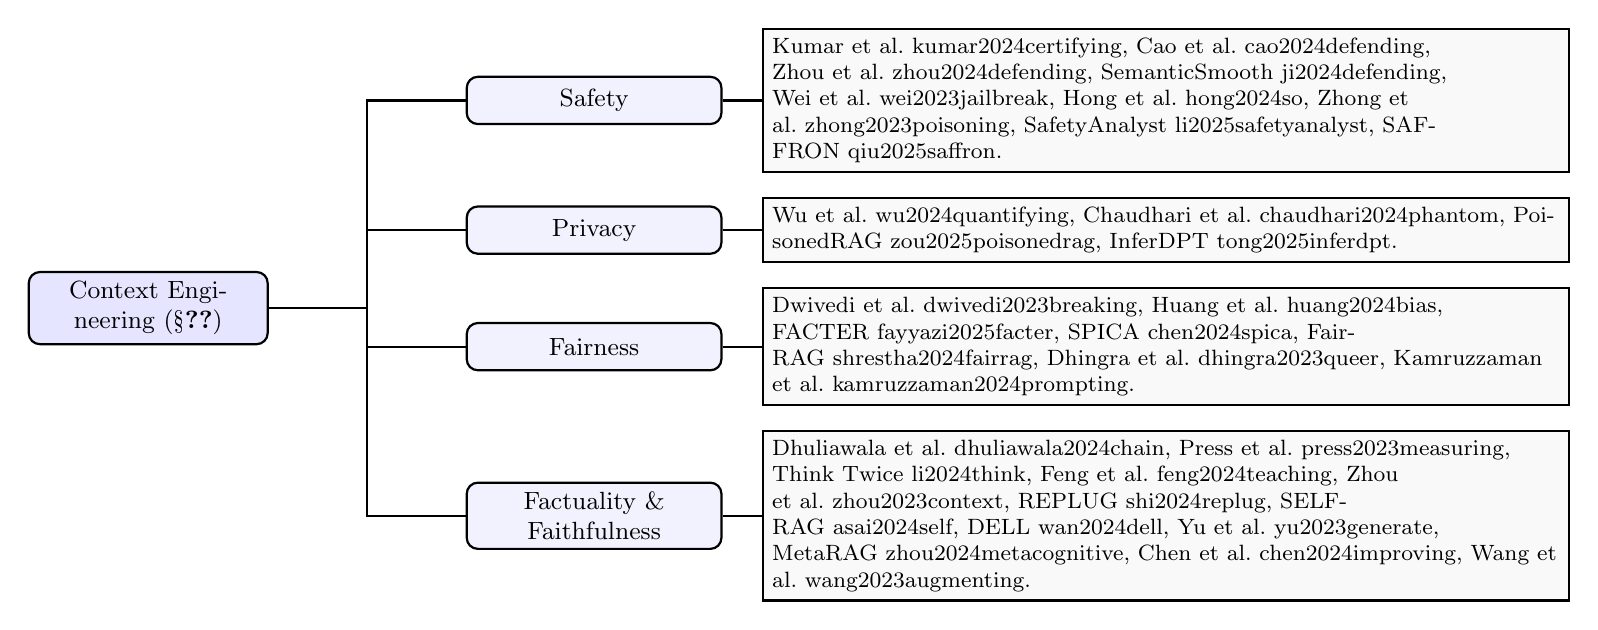
\begin{tikzpicture}
        % --- 1. Define leaf nodes (papers, citations added) ---
        \node[leaf] (safety_papers) {
            Kumar et al.~\citep{kumar2024certifying}, Cao et al.~\citep{cao2024defending}, Zhou et al.~\citep{zhou2024defending}, SemanticSmooth~\citep{ji2024defending}, Wei et al.~\citep{wei2023jailbreak}, Hong et al.~\citep{hong2024so}, Zhong et al.~\citep{zhong2023poisoning}, SafetyAnalyst~\citep{li2025safetyanalyst}, SAFFRON~\citep{qiu2025saffron}.
        };
        \node[leaf, below=0.3cm of safety_papers] (privacy_papers) {
            Wu et al.~\citep{wu2024quantifying}, Chaudhari et al.~\citep{chaudhari2024phantom}, PoisonedRAG~\citep{zou2025poisonedrag}, InferDPT~\citep{tong2025inferdpt}.
        };
        \node[leaf, below=0.3cm of privacy_papers] (fairness_papers) {
            Dwivedi et al.~\citep{dwivedi2023breaking}, Huang et al.~\citep{huang2024bias}, FACTER~\citep{fayyazi2025facter}, SPICA~\citep{chen2024spica}, FairRAG~\citep{shrestha2024fairrag}, Dhingra et al.~\citep{dhingra2023queer}, Kamruzzaman et al.~\citep{kamruzzaman2024prompting}.
        };
        \node[leaf, below=0.3cm of fairness_papers] (factuality_papers) {
            Dhuliawala et al.~\citep{dhuliawala2024chain}, Press et al.~\citep{press2023measuring}, Think Twice~\citep{li2024think}, Feng et al.~\citep{feng2024teaching}, Zhou et al.~\citep{zhou2023context}, REPLUG~\citep{shi2024replug}, SELF-RAG~\citep{asai2024self}, DELL~\citep{wan2024dell}, Yu et al.~\citep{yu2023generate}, MetaRAG~\citep{zhou2024metacognitive}, Chen et al.~\citep{chen2024improving}, Wang et al.~\citep{wang2023augmenting}.
        };

        % --- 2. Define main sub-nodes (Trustworthiness dimensions) ---
        \node[sub, left=0.5cm of safety_papers] (safety) {Safety};
        \node[sub, left=0.5cm of privacy_papers] (privacy) {Privacy};
        \node[sub, left=0.5cm of fairness_papers] (fairness) {Fairness};
        \node[sub, left=0.5cm of factuality_papers] (factuality) {Factuality \&  Faithfulness};

        % --- 3. Define root node ---
        \node[main, left=2.5cm of {$(safety.west)!0.5!(factuality.west)$}] (ce) {Context Engineering (§\ref{sec:context_engineering})};

        % --- 4. Draw connection lines ---
        % a. Draw a main trunk from the root node to a branching point
        \coordinate (fork) at ($(ce.east) + (1.25cm,0)$);
        \draw[line] (ce.east) -- (fork);

        % b. Connect from main branching point to each sub-node
        \draw[line] (fork) |- (safety.west);
        \draw[line] (fork) |- (privacy.west);
        \draw[line] (fork) |- (fairness.west);
        \draw[line] (fork) |- (factuality.west);

        % c. Connect main sub-nodes directly to leaf nodes
        \draw[line] (safety.east) -- (safety_papers.west);
        \draw[line] (privacy.east) -- (privacy_papers.west);
        \draw[line] (fairness.east) -- (fairness_papers.west);
        \draw[line] (factuality.east) -- (factuality_papers.west);

        \end{tikzpicture}%
    }
    \caption{A taxonomy of Context Engineering for enhancing LLM trustworthiness.}
    \label{fig:ce_taxonomy}
\end{figure}

Within the landscape of inference-time methods for trustworthy LLMs, context engineering (CE) has emerged as a central paradigm. Instead of modifying model parameters, CE emphasizes the deliberate design and orchestration of the information presented to the model at inference time. This approach is particularly important for trustworthiness: by shaping the context, one can systematically influence factuality, safety, fairness, etc, without modifying model's parameters.

\subsubsection{Core Principle}

Context engineering is the systematic discipline of designing, optimizing, and managing the information payload provided to LLMs at inference time. Unlike early prompt engineering, which treated the context as a flat string, CE models the context as a structured composition of four components: directive instructions encompassing rules and constraints; knowledge inputs such as retrieved documents or prior dialogue; interaction mechanisms including tools, APIs, or system affordances; and the live user query specifying the task at hand. An assembly function integrates these heterogeneous elements into the final sequence consumed by the model.

The CE framework rests on three foundational pillars that together form a pipeline. Context retrieval and generation is responsible for sourcing task-relevant material through prompt design, retrieval from external knowledge bases, and adaptive assembly strategies. Context processing transforms raw material into model-ready input through compression, refinement, and multimodal or structured integration. Context management ensures coherence and efficiency across stages by dynamically organizing, prioritizing, and updating contextual elements under system constraints such as the maximum context length. Together, these pillars support higher-level methods such as Retrieval-Augmented Generation (RAG), persistent memory, tool-augmented reasoning, and multi-agent collaboration.


\subsubsection{Applications}

\paragraph{Safety}

Context engineering promotes safety by controlling the informational boundary within which a model operates, encoding explicit constraints at the prompt level, grounding generation in trusted external sources, and embedding verification routines into the reasoning process. Prompt engineering offers a lightweight first layer of defense, ranging from certifiable defenses with robustness guarantees against adversarial prompts~\citep{kumar2024certifying} and robust alignment prompting~\citep{cao2024defending} to baseline defenses such as paraphrasing, in-context refusals, and perplexity checks~\citep{zhou2024defending}, as well as smoothing-based methods like SemanticSmooth that guard against both token- and prompt-level attacks~\citep{ji2024defending}. Retrieval-augmented generation further enhances safety by grounding responses in verifiable external knowledge, reducing hallucinations and lowering the risk of unsafe misinformation~\citep{wei2023jailbreak, hong2024so}, though vulnerabilities such as corpus poisoning attacks that insert adversarial passages into knowledge bases remain a concern~\citep{zhong2023poisoning}. Reasoning-oriented approaches complement these strategies by enabling models to regulate their own outputs during inference through structured step-by-step verification~\citep{li2025safetyanalyst} and safety-aware scoring that resists jailbreaks at scale~\citep{qiu2025saffron}.

\paragraph{Privacy}

Context engineering for privacy focuses on controlling what enters the model's context. Instead of modifying parameters, privacy is preserved by assembling the context such that sensitive elements are masked, filtered, or abstracted while retaining task-relevant information. Recent work shows that CE can both introduce and mitigate privacy risks. Prompts themselves may leak sensitive training data through property and membership inference attacks~\citep{wu2024quantifying}, and RAG pipelines are vulnerable to poisoned documents that can exfiltrate private passages or bias model outputs~\citep{chaudhari2024phantom}. On the defense side, certified privacy-preserving mechanisms for RAG offer robustness against adversarial manipulation~\citep{zou2025poisonedrag}, while frameworks for selective retrieval and privacy-aware generation control personal data exposure~\citep{tong2025inferdpt}. Together, these studies underscore that privacy risks often stem from how external context is engineered into models, and effective mitigation requires careful control, sanitization, and certification of injected information.

\paragraph{Fairness}

Bias in LLMs often arises from skewed training data and emergent model behavior, and context engineering provides a practical means of mitigation without retraining. Carefully designed prompts have been shown to reduce bias, from employing in-context learning to mitigate gender stereotypes~\citep{dwivedi2023breaking} to frameworks for testing and reducing social bias in code generation through iterative, feedback-driven prompting~\citep{huang2024bias} and embedding explicit fairness constraints in prompts~\citep{fayyazi2025facter}. Retrieval-augmented methods enhance fairness by grounding outputs in curated, balanced evidence, with fairness-aware retrieval mechanisms prioritizing diverse and representative sources to reduce stereotype reinforcement~\citep{chen2024spica, shrestha2024fairrag}. A third line of work integrates structured reasoning through chain-of-thought~\citep{dhingra2023queer} or deliberative reasoning~\citep{kamruzzaman2024prompting} to enforce fairness constraints, decomposing decisions into interpretable steps that enable bias detection and correction during inference.

\paragraph{Factuality}

A core challenge in trustworthy AI is mitigating factual errors and hallucinations, and context engineering offers several complementary strategies. Prompt engineering improves factual consistency through structured instructions, including self-detection prompts that require models to evaluate multiple candidate answers before finalizing a response~\citep{dhuliawala2024chain, press2023measuring, li2024think}, abstention-oriented prompting that encourages models to decline uncertain answers in multilingual settings~\citep{feng2024teaching}, and opinion-based or counterfactual demonstrations that reduce reliance on parametric knowledge~\citep{zhou2023context}. Retrieval-augmented generation enhances factual grounding by supplementing LLMs with external documents, with frameworks enabling adaptive and reflective retrieval such as SELF-RAG~\citep{asai2024self}, integration of retrieval with proxy explanations for misinformation detection~\citep{wan2024dell, yu2023generate, shi2024replug}, and metacognitive loops that detect insufficient or conflicting knowledge and adjust retrieval accordingly~\citep{zhou2024metacognitive}. Memory-based methods further improve factuality by allowing models to retain and update knowledge across interactions through external memory buffers where user feedback persists across sessions~\citep{chen2024improving} and modular memory systems combining episodic traces and semantic caches~\citep{wang2023augmenting}.

%% ============================================================
%% Revision Notes (2026-03-29, Yuyang):
%% 1. Core Principle: Already concise, kept as-is.
%% 2. Typology of Guardrail Mechanisms: Shortened each type description,
%%    especially Model-Based (compressed historical toxicity detection work).
%% 3. Applications: Split combined Safety+Privacy and Fairness+Factuality
%%    paragraphs into four separate \paragraph entries, one per domain.
%% 4. Discussion: Removed from this file. Shortened version moved to
%%    sections/11-challenges_directions.tex with red source marker.
%% ============================================================

\subsection{Guardrails}
\label{sec:guardrails}

\begin{figure}[htbp]
\centering
% Width uses \textwidth; height auto-scales with !
\resizebox{\textwidth}{!}{%
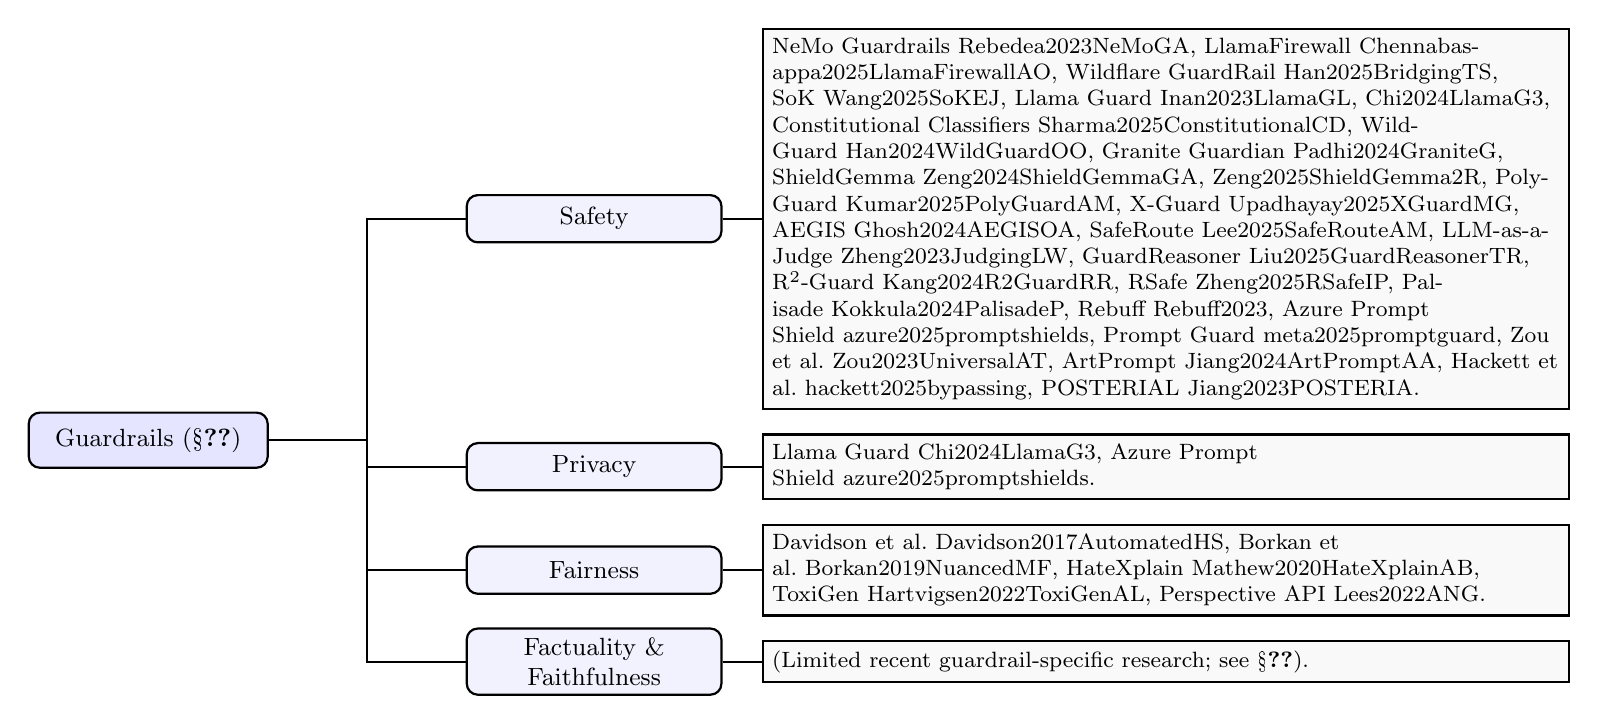
\begin{tikzpicture}
% --- 1. Define leaf nodes (papers, citations added) ---
\node[leaf] (safety_papers) {
NeMo Guardrails~\citep{Rebedea2023NeMoGA}, LlamaFirewall~\citep{Chennabasappa2025LlamaFirewallAO}, Wildflare GuardRail~\citep{Han2025BridgingTS}, SoK~\citep{Wang2025SoKEJ}, Llama Guard~\citep{Inan2023LlamaGL, Chi2024LlamaG3}, Constitutional Classifiers~\citep{Sharma2025ConstitutionalCD}, WildGuard~\citep{Han2024WildGuardOO}, Granite Guardian~\citep{Padhi2024GraniteG}, ShieldGemma~\citep{Zeng2024ShieldGemmaGA, Zeng2025ShieldGemma2R}, PolyGuard~\citep{Kumar2025PolyGuardAM}, X-Guard~\citep{Upadhayay2025XGuardMG}, AEGIS~\citep{Ghosh2024AEGISOA}, SafeRoute~\citep{Lee2025SafeRouteAM}, LLM-as-a-Judge~\citep{Zheng2023JudgingLW}, GuardReasoner~\citep{Liu2025GuardReasonerTR}, R$^2$-Guard~\citep{Kang2024R2GuardRR}, RSafe~\citep{Zheng2025RSafeIP}, Palisade~\citep{Kokkula2024PalisadeP}, Rebuff~\citep{Rebuff2023}, Azure Prompt Shield~\citep{azure2025promptshields}, Prompt Guard~\citep{meta2025promptguard}, Zou et al.~\citep{Zou2023UniversalAT}, ArtPrompt~\citep{Jiang2024ArtPromptAA}, Hackett et al.~\citep{hackett2025bypassing}, POSTERIAL~\citep{Jiang2023POSTERIA}.
};
\node[leaf, below=0.3cm of safety_papers] (privacy_papers) {
Llama Guard~\citep{Chi2024LlamaG3}, Azure Prompt Shield~\citep{azure2025promptshields}.
};
\node[leaf, below=0.3cm of privacy_papers] (fairness_papers) {
Davidson et al.~\citep{Davidson2017AutomatedHS}, Borkan et al.~\citep{Borkan2019NuancedMF}, HateXplain~\citep{Mathew2020HateXplainAB}, ToxiGen~\citep{Hartvigsen2022ToxiGenAL}, Perspective API~\citep{Lees2022ANG}.
};
\node[leaf, below=0.3cm of fairness_papers] (factuality_papers) {
(Limited recent guardrail-specific research; see §\ref{sec:guardrails}).
};
% --- 2. Define main sub-nodes (Trustworthiness dimensions) ---
% Positioned to the left of corresponding leaf nodes
\node[sub, left=0.5cm of safety_papers] (safety) {Safety};
\node[sub, left=0.5cm of privacy_papers] (privacy) {Privacy};
\node[sub, left=0.5cm of fairness_papers] (fairness) {Fairness};
\node[sub, left=0.5cm of factuality_papers] (factuality) {Factuality \& Faithfulness};
% --- 3. Define root node ---
% Use the calc library to vertically center the root node relative to the sub-nodes
\node[main, left=2.5cm of {$(safety.west)!0.5!(factuality.west)$}] (guardrails) {Guardrails (§\ref{sec:guardrails})};
% --- 4. Draw connection lines ---
% a. Draw a main trunk from the root node to a branching point
\coordinate (fork) at ($(guardrails.east)+(1.25cm,0)$);
\draw[line] (guardrails.east) -- (fork);
% b. Connect from main branching point to each sub-node
\draw[line] (fork) |- (safety.west);
\draw[line] (fork) |- (privacy.west);
\draw[line] (fork) |- (fairness.west);
\draw[line] (fork) |- (factuality.west);
% c. Connect main sub-nodes directly to leaf nodes
\draw[line] (safety.east) -- (safety_papers.west);
\draw[line] (privacy.east) -- (privacy_papers.west);
\draw[line] (fairness.east) -- (fairness_papers.west);
\draw[line] (factuality.east) -- (factuality_papers.west);
\end{tikzpicture}%
}
\caption{A taxonomy of Guardrails for enhancing LLM trustworthiness.}
\label{fig:guardrails_taxonomy}
\end{figure}

\subsubsection{Core Principle: Modular and External Control}

Guardrails provide a modular and external mechanism for controlling LLM behavior, operating as independent components that monitor and filter inputs or outputs without modifying the model's parameters. Unlike training-time interventions, guardrails function post-deployment, treating the LLM as a black-box system. This external positioning enables rapid deployment and updates, allowing systems to quickly adapt to evolving safety requirements and emerging threats. Their modular design supports flexible integration into existing pipelines, where multiple guardrails can be layered or combined to target specific risks. As external controls, guardrails ensure trustworthy outputs by intercepting potentially harmful content before it reaches the user or by regenerating outputs when violations are detected. While this  principle draws conceptually from traditional content moderation systems, it is now tailored to the dynamic and interactive nature of LLMs, emphasizing flexibility and minimal interference with the model's core functionality.

\begin{figure*}[htbp]
  \centering
  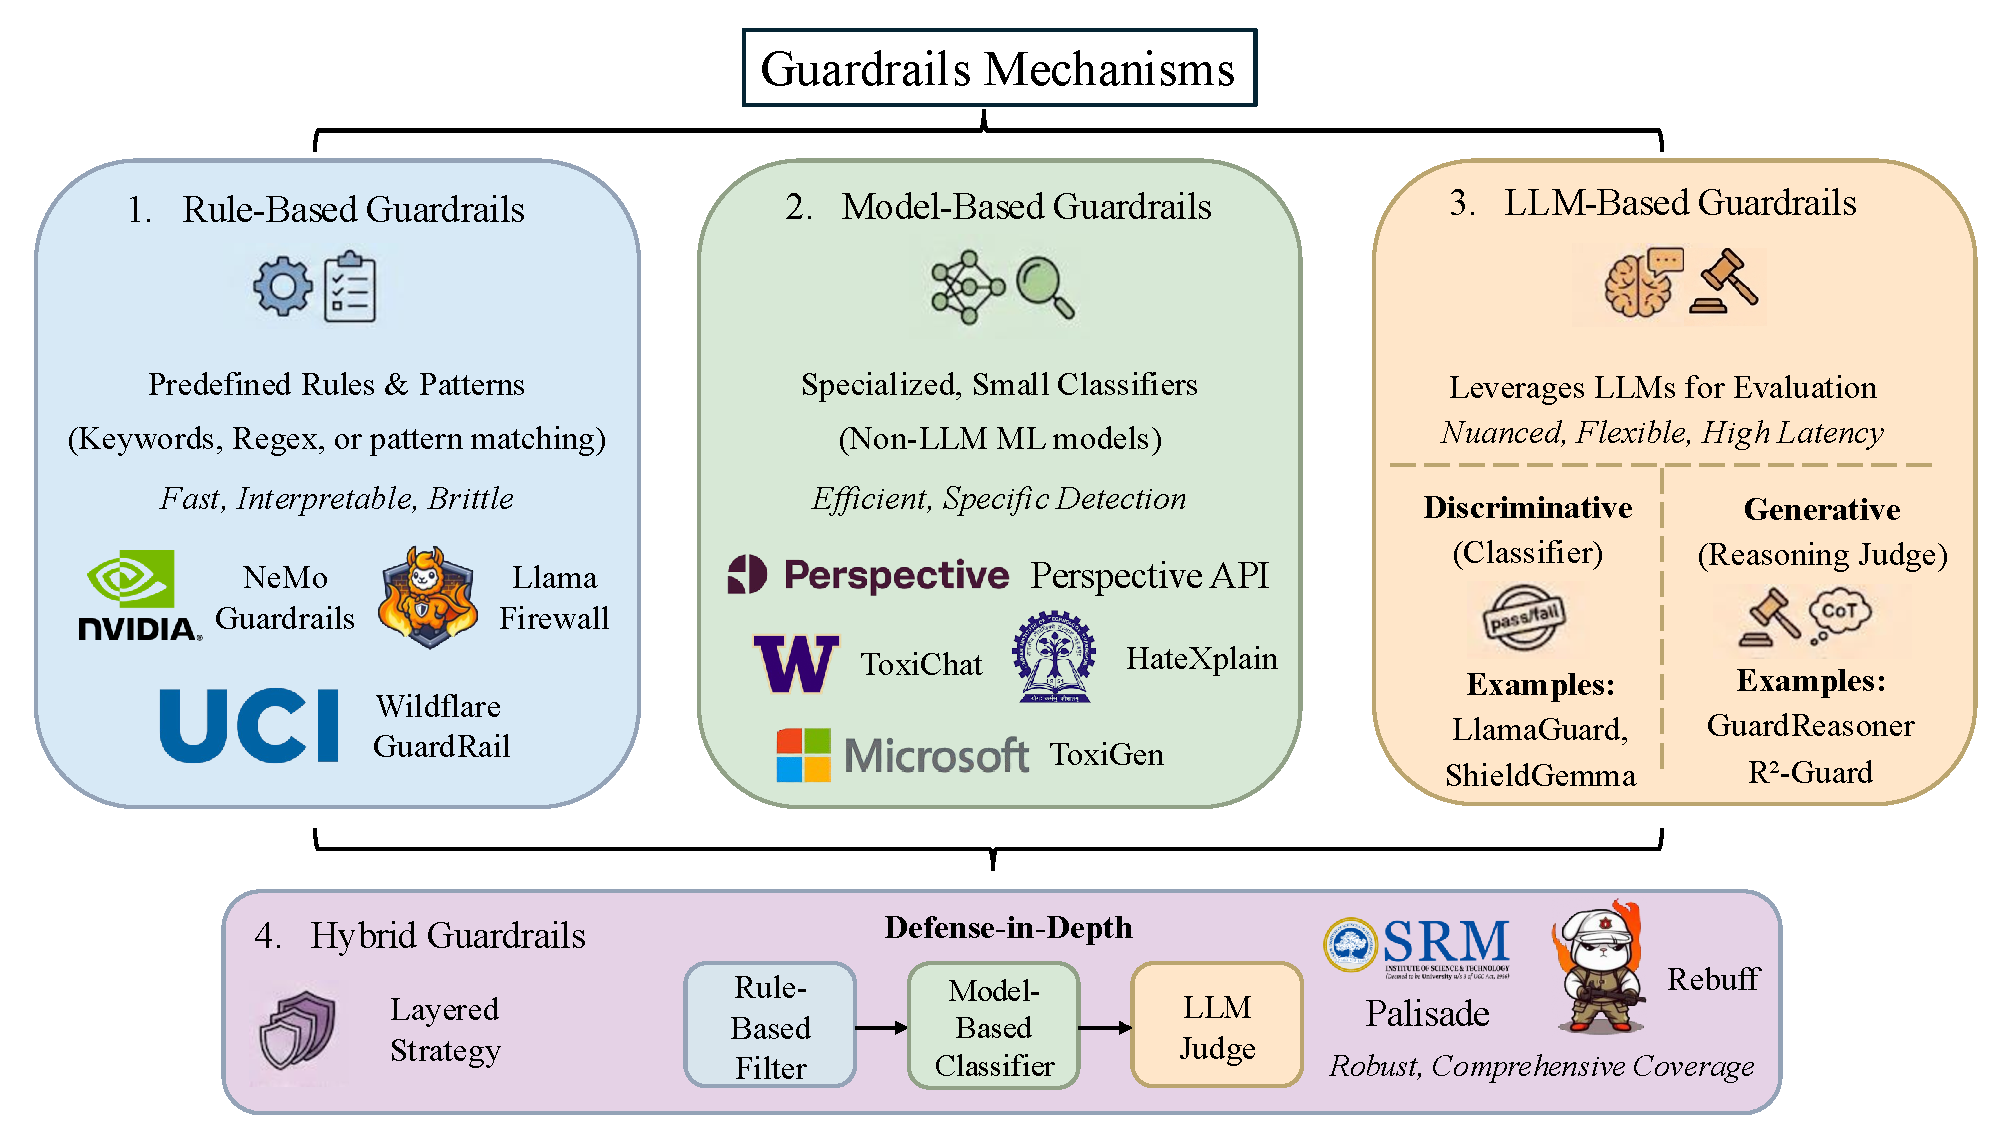
\includegraphics[width=0.9\linewidth]{figures/method/guardrails_new.pdf}
  \caption{A typology of guardrail mechanisms for LLM trustworthiness. The four categories---Rule-Based, Model-Based, LLM-Based (discriminative and generative), and Hybrid---are distinguished by their underlying detection approach, with representative systems shown for each. Hybrid guardrails combine multiple mechanism types in a layered ``defense-in-depth'' strategy for comprehensive coverage.}
  \label{fig:method_guardrails}
\end{figure*}


\subsubsection{A Typology of Guardrail Mechanisms}

Guardrail mechanisms can be classified according to their underlying approach, spanning from simple deterministic techniques to advanced LLM-driven systems.

\paragraph{Rule-Based Guardrails}

Rule-based guardrails rely on predefined rules, such as keyword lists, regular expressions, or pattern matching, to detect and filter prohibited content. For example, NeMo Guardrails~\citep{Rebedea2023NeMoGA} introduces programmable rails for dialog flow, topic blocking, and tool use; LlamaFirewall~\citep{Chennabasappa2025LlamaFirewallAO} incorporates customizable scanners including regex-based code filters for agentic workflows; and Wildflare GuardRail~\citep{Han2025BridgingTS} integrates modular rule-based wrappers as part of a multi-stage pipeline. While transparent and low-latency, these systems are brittle against novel adversarial strategies specific to LLMs, such as prompt injection and jailbreak attacks~\citep{Wang2025SoKEJ}.

\paragraph{Model-Based Guardrails}

Model-based guardrails employ smaller, specialized classifiers---typically non-LLM models such as neural networks or fine-tuned smaller transformers---for nuanced detection of safety violations. Early work focused on hate speech and toxicity detection, addressing challenges such as distinguishing hate speech from offensive content~\citep{Davidson2017AutomatedHS}, fairness-oriented evaluation for toxicity detectors~\citep{Borkan2019NuancedMF}, and adversarially generated datasets for implicit toxicity~\citep{Hartvigsen2022ToxiGenAL}. These insights informed practical deployments such as the Perspective API~\citep{Lees2022ANG}, which detects toxicity across languages, and explainable models like HateXplain~\citep{Mathew2020HateXplainAB} that provide human rationales alongside labels.

\paragraph{LLM-Based Guardrails}

LLM-based guardrails employ another large language model to evaluate and filter generated content, capturing nuance, abstraction, and intent that smaller classifiers often miss. Discriminative guardrails use LLMs as safety classifiers: Llama Guard~\citep{Inan2023LlamaGL, Chi2024LlamaG3} detects unsafe multimodal content categories, while Constitutional Classifiers~\citep{Sharma2025ConstitutionalCD}, WildGuard~\citep{Han2024WildGuardOO}, Granite Guardian~\citep{Padhi2024GraniteG}, and ShieldGemma~\citep{Zeng2024ShieldGemmaGA, Zeng2025ShieldGemma2R} provide fine-tuned drop-in safety classifiers. Recent work has expanded to multilingual coverage with PolyGuard~\citep{Kumar2025PolyGuardAM} and X-Guard~\citep{Upadhayay2025XGuardMG}, while ensemble approaches like AEGIS~\citep{Ghosh2024AEGISOA} and adaptive routing via SafeRoute~\citep{Lee2025SafeRouteAM} reflect a shift toward scalable, real-time solutions. Generative (reasoning) guardrails employ an LLM as a deliberative judge that critiques and justifies another model's output. Building on the LLM-as-a-judge paradigm~\citep{Zheng2023JudgingLW}, recent methods incorporate explicit reasoning chains before producing verdicts, such as GuardReasoner~\citep{Liu2025GuardReasonerTR}, R$^2$-Guard~\citep{Kang2024R2GuardRR} with knowledge-enhanced logical reasoning, GuardAdvisor~\citep{huang2026guardian} with a soft-gating pipeline, and RSafe~\citep{Zheng2025RSafeIP} with adaptive guided safety reasoning.

\paragraph{Hybrid Guardrails}

Hybrid guardrails combine multiple mechanisms for comprehensive coverage through a ``defense-in-depth'' strategy. For example, Palisade~\citep{Kokkula2024PalisadeP} proposes a three-layer pipeline combining a rule-based filter, an ML classifier, and a companion-LLM check, while Rebuff~\citep{Rebuff2023} integrates heuristics, canary tokens, a database of known attacks, and an LLM-based check.

\subsubsection{Applications}

\paragraph{Safety}

Guardrails are predominantly applied in safety, where they serve as critical defenses against emerging threats inherent to LLMs. On the input side, guardrails detect and block attacks such as jailbreaks that aim to bypass alignment constraints~\citep{Zou2023UniversalAT, Jiang2024ArtPromptAA} and prompt injections where adversaries embed malicious instructions to hijack model outputs~\citep{hackett2025bypassing, Jiang2023POSTERIA}. Systems like Azure Prompt Shield~\citep{azure2025promptshields} and Prompt Guard~\citep{meta2025promptguard} employ adversarial-input detectors to identify injection attempts and block unsafe prompts. On the output side, guardrails evaluate and filter model generations before delivery to end users, with systems like Llama Guard~\citep{Chi2024LlamaG3} enforcing a taxonomy of unsafe categories---including violent crimes, sex crimes and child exploitation, defamation, hate speech, self-harm, and election misinformation---by classifying outputs and blocking or regenerating unsafe completions.

\paragraph{Privacy}

In the privacy domain, guardrails protect against the disclosure of personal or sensitive information. Output-side guardrails can classify and block generations that contain personally identifiable information, confidential data, or intellectual property violations. Systems such as Llama Guard~\citep{Chi2024LlamaG3} include disclosure of sensitive information as an explicit unsafe category, while Azure Prompt Shield~\citep{azure2025promptshields} detects attempts to exfiltrate private data through prompt injection. However, guardrail-specific research for privacy remains limited compared to safety, and most privacy protections are currently bundled within broader safety taxonomies rather than addressed by dedicated guardrail mechanisms.

\paragraph{Fairness}

Guardrails for fairness have historical roots in pre-LLM content moderation, where classifiers were designed to detect and reduce bias in generated content~\citep{Borkan2019NuancedMF, Mathew2020HateXplainAB}. Toxicity and hate speech detectors such as Perspective API~\citep{Lees2022ANG} and ToxiGen classifiers~\citep{Hartvigsen2022ToxiGenAL} serve as fairness-oriented guardrails by flagging content that disparages or stereotypes specific demographic groups. In the LLM era, however, fairness-specific guardrail research has received less attention, likely due to the assumption that post-training alignment methods such as RLHF improve baseline fairness, leaving a gap for dedicated fairness enforcement mechanisms at inference time.

\paragraph{Factuality}

Guardrails for factuality represent the least developed dimension in current research. While output-side guardrails could in principle verify factual claims against trusted knowledge bases or flag low-confidence generations, there is limited recent work on dedicated factuality-focused guardrail mechanisms for LLMs. This gap presents an opportunity for future research to develop fact-checking guardrails that complement retrieval-augmented and decoding-based approaches to factual grounding.

%% ============================================================
%% Revision Notes (2026-03-29, Yuyang):
%% 1. Core Principle: Removed mathematical formulation (autoregressive
%%    equation) and decoding strategy enumeration. Kept concise prose
%%    description of real-time logit/probability manipulation.
%% 2. Applications: Merged sub-categories (Contrastive/External Guidance/
%%    Context-Adaptive/Specialized/Reference-Based etc.) into one
%%    paragraph per trustworthiness domain. Removed \textbf sub-headings.
%% 3. Discussion: Removed from this file. Shortened version moved to
%%    sections/11-challenges_directions.tex with red source marker.
%% ============================================================

\subsection{Decoding}
\label{sec:decoding}

\begin{figure}[htbp]
\centering
% Width uses \textwidth; height auto-scales with !
\resizebox{\textwidth}{!}{%
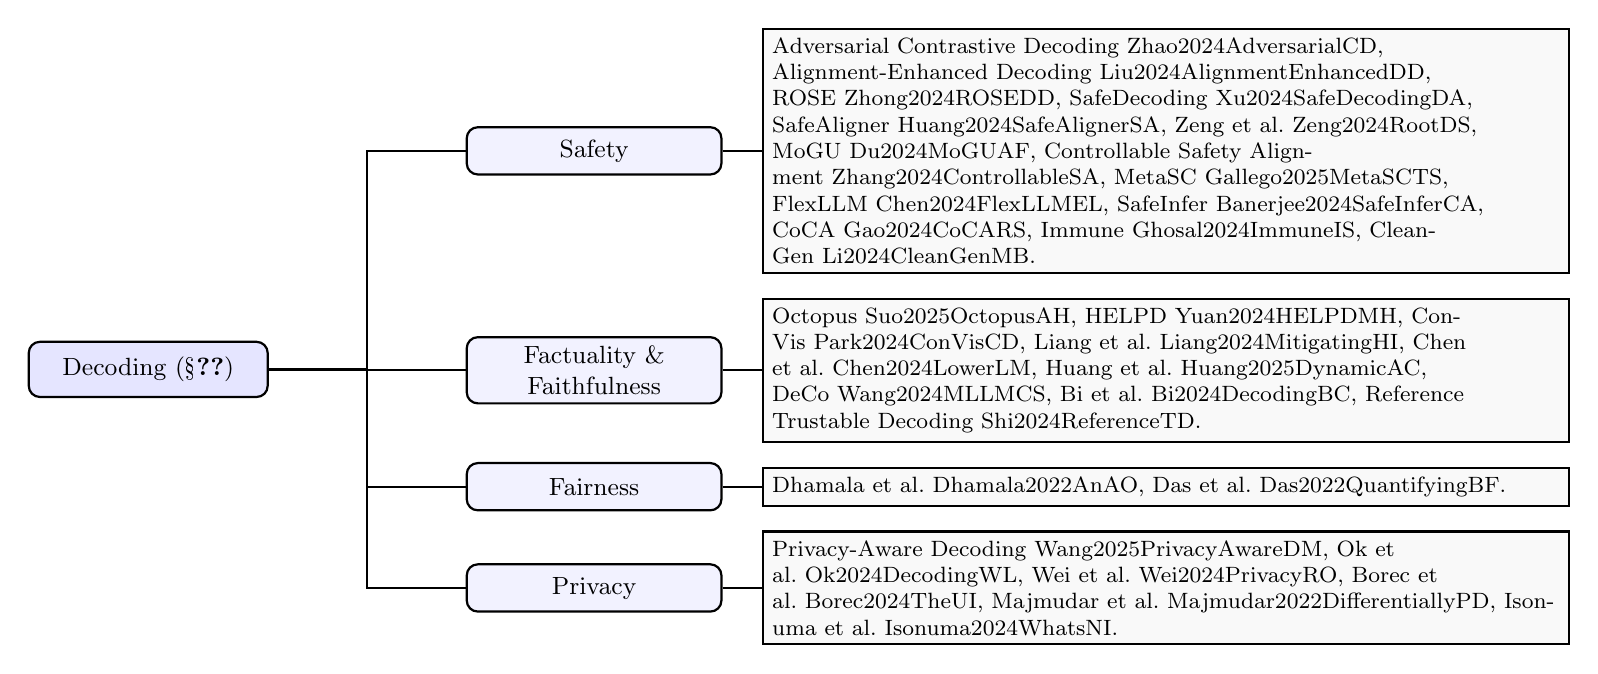
\begin{tikzpicture}
% --- 1. Define leaf nodes (papers, citations added) ---
\node[leaf] (safety_papers) {
Adversarial Contrastive Decoding~\citep{Zhao2024AdversarialCD}, Alignment-Enhanced Decoding~\citep{Liu2024AlignmentEnhancedDD}, ROSE~\citep{Zhong2024ROSEDD}, SafeDecoding~\citep{Xu2024SafeDecodingDA}, SafeAligner~\citep{Huang2024SafeAlignerSA}, Zeng et al.~\citep{Zeng2024RootDS}, MoGU~\citep{Du2024MoGUAF}, Controllable Safety Alignment~\citep{Zhang2024ControllableSA}, MetaSC~\citep{Gallego2025MetaSCTS}, FlexLLM~\citep{Chen2024FlexLLMEL}, SafeInfer~\citep{Banerjee2024SafeInferCA}, CoCA~\citep{Gao2024CoCARS}, Immune~\citep{Ghosal2024ImmuneIS}, CleanGen~\citep{Li2024CleanGenMB}.
};
\node[leaf, below=0.3cm of safety_papers] (factuality_papers) {
Octopus~\citep{Suo2025OctopusAH}, HELPD~\citep{Yuan2024HELPDMH}, ConVis~\citep{Park2024ConVisCD}, Liang et al.~\citep{Liang2024MitigatingHI}, Chen et al.~\citep{Chen2024LowerLM}, Huang et al.~\citep{Huang2025DynamicAC}, DeCo~\citep{Wang2024MLLMCS}, Bi et al.~\citep{Bi2024DecodingBC}, Reference Trustable Decoding~\citep{Shi2024ReferenceTD}.
};
\node[leaf, below=0.3cm of factuality_papers] (fairness_papers) {
Dhamala et al.~\citep{Dhamala2022AnAO}, Das et al.~\citep{Das2022QuantifyingBF}.
};
\node[leaf, below=0.3cm of fairness_papers] (privacy_papers) {
Privacy-Aware Decoding~\citep{Wang2025PrivacyAwareDM}, Ok et al.~\citep{Ok2024DecodingWL}, Wei et al.~\citep{Wei2024PrivacyRO}, Borec et al.~\citep{Borec2024TheUI}, Majmudar et al.~\citep{Majmudar2022DifferentiallyPD}, Isonuma et al.~\citep{Isonuma2024WhatsNI}.
};
% --- 2. Define main sub-nodes (Trustworthiness dimensions) ---
% Positioned to the left of corresponding leaf nodes
\node[sub, left=0.5cm of safety_papers] (safety) {Safety};
\node[sub, left=0.5cm of factuality_papers] (factuality) {Factuality \& Faithfulness};
\node[sub, left=0.5cm of fairness_papers] (fairness) {Fairness};
\node[sub, left=0.5cm of privacy_papers] (privacy) {Privacy};
% --- 3. Define root node ---
% Use the calc library to vertically center the root node relative to the sub-nodes
\node[main, left=2.5cm of {$(safety.west)!0.5!(privacy.west)$}] (decoding) {Decoding (§\ref{sec:decoding})};
% --- 4. Draw connection lines ---
% a. Draw a main trunk from the root node to a branching point
\coordinate (fork) at ($(decoding.east)+(1.25cm,0)$);
\draw[line] (decoding.east) -- (fork);
% b. Connect from main branching point to each sub-node
\draw[line] (fork) |- (safety.west);
\draw[line] (fork) |- (factuality.west);
\draw[line] (fork) |- (fairness.west);
\draw[line] (fork) |- (privacy.west);
% c. Connect main sub-nodes directly to leaf nodes
\draw[line] (safety.east) -- (safety_papers.west);
\draw[line] (factuality.east) -- (factuality_papers.west);
\draw[line] (fairness.east) -- (fairness_papers.west);
\draw[line] (privacy.east) -- (privacy_papers.west);
\end{tikzpicture}%
}
\caption{A taxonomy of Decoding Strategies for enhancing LLM trustworthiness.}
\label{fig:decoding_taxonomy}
\end{figure}

\subsubsection{Core Principle: Real-Time Logit and Probability Manipulation}

Decoding strategies involve real-time manipulation of the token probability distribution or logits at each generation step to steer the model's outputs toward desired characteristics. At each step, the model produces a probability distribution over its vocabulary conditioned on the preceding tokens, and decoding interventions modify this distribution---by suppressing, amplifying, or re-weighting specific token probabilities---before sampling the next token. This approach allows for fine-grained control over output without modifying the model's parameters, making it computationally efficient and adaptable to diverse trustworthiness requirements.

\begin{figure*}[htbp]
  \centering
  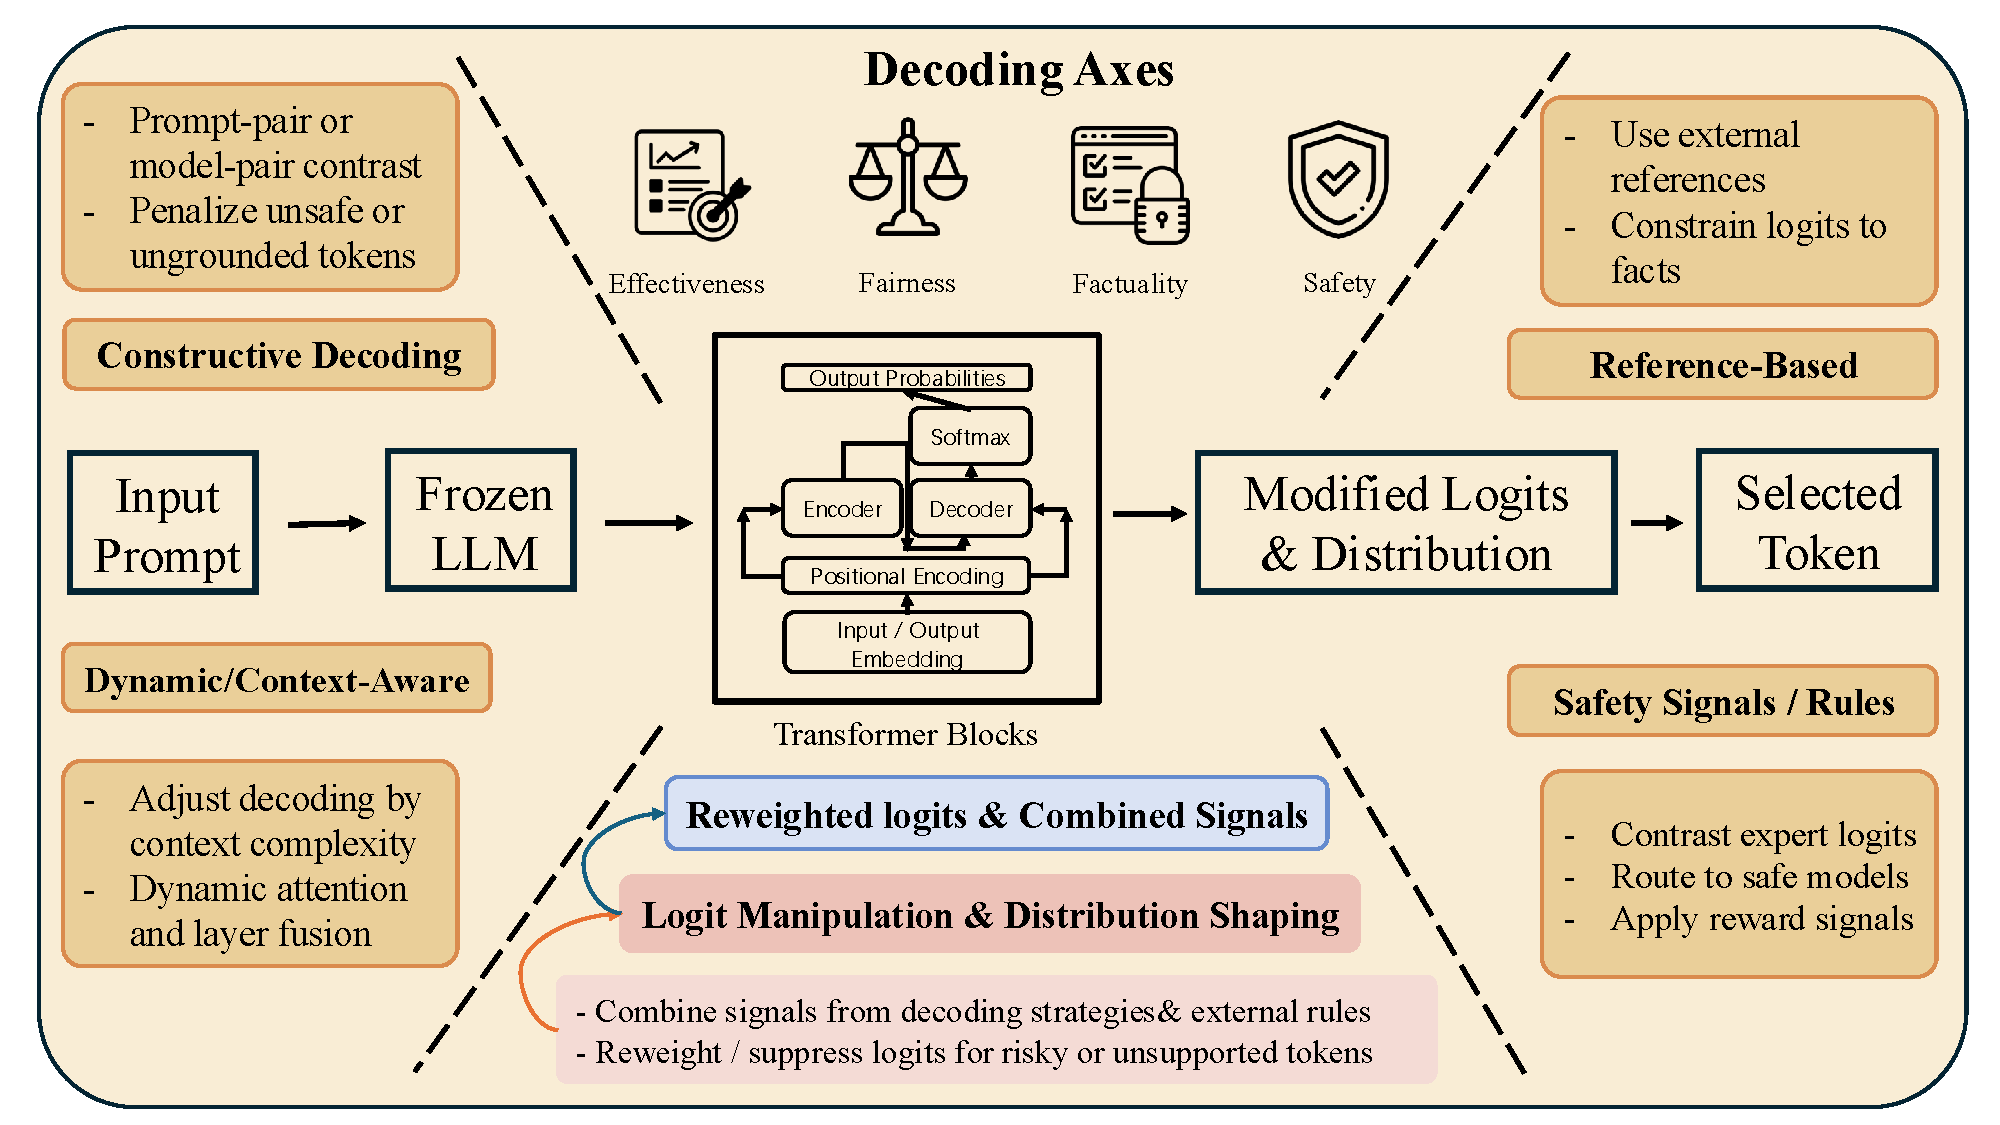
\includegraphics[width=0.9\linewidth]{figures/method/decoding_new2.pdf}
  \caption{Overview of trustworthiness-oriented decoding strategies. A frozen LLM produces logits that are modified at each autoregressive step by three complementary families of interventions before token sampling. \textbf{Contrastive Decoding} (balance icon) contrasts outputs from paired prompts or paired models---e.g., safe versus unsafe prompts, or an expert against an amateur model---to penalize unsafe or ungrounded tokens. \textbf{Dynamic/Context-Aware Decoding} (neural-network icon) adjusts decoding hyperparameters, attention weights, or layer fusion on the fly, based on context complexity or intermediate signals. \textbf{Reference-Based Decoding} (document-with-shield icon) constrains logits toward facts or safety policies sourced from external references such as retrieved documents or rule sets. These three families feed into a shared \emph{Logit Manipulation \& Distribution Shaping} stage, optionally combined with external knowledge or safety signals, which reweights or suppresses risky, unsupported, or unsafe tokens before the next token is sampled.}
  \label{fig:method_decoding}
\end{figure*}


\subsubsection{Applications}

\paragraph{Safety}

Decoding strategies for safety center on inference-time intervention to prevent harmful outputs without altering model weights, and are crucial for defending against adversarial attacks such as jailbreaks. Contrastive decoding enhances safety by comparing logits from safe and unsafe distributions: methods like Adversarial Contrastive Decoding~\citep{Zhao2024AdversarialCD} and Alignment-Enhanced Decoding~\citep{Liu2024AlignmentEnhancedDD} use opposite or malicious prompts to penalize unsafe continuations, while SafeDecoding~\citep{Xu2024SafeDecodingDA} and SafeAligner~\citep{Huang2024SafeAlignerSA} contrast logits from safety-trained expert models against base or unsafe models, and ROSE~\citep{Zhong2024ROSEDD} applies reverse prompt contrastive decoding with step-by-step correction~\citep{Zeng2024RootDS}. External guidance approaches use separate models or signals to steer generation, such as MoGU's dynamic routing between a usable and a safe LLM~\citep{Du2024MoGUAF}, inference-time adaptation through safety configurations~\citep{Zhang2024ControllableSA}, and meta-critique optimization of safety specifications~\citep{Gallego2025MetaSCTS}. Context-adaptive and dynamic defenses adjust safety measures based on specific inputs, including moving target defense through dynamic decoding hyper-parameters~\citep{Chen2024FlexLLMEL} and context-adaptive safety amplification~\citep{Banerjee2024SafeInferCA}. Specialized defense work addresses safety in multimodal LLMs through output distribution calibration~\citep{Gao2024CoCARS} and safety reward model alignment~\citep{Ghosal2024ImmuneIS}, as well as countering backdoor attacks via speculative decoding to identify suspicious tokens~\citep{Li2024CleanGenMB}.

\paragraph{Factuality}

Diverse decoding strategies have been developed to mitigate hallucinations and ensure context-aware outputs in LLMs and MLLMs. Contrastive decoding reduces hallucinations by contrasting output distributions derived from original and perturbed inputs: Octopus~\citep{Suo2025OctopusAH} adapts to input complexity with noise, HELPD~\citep{Yuan2024HELPDMH} employs hierarchical feedback with vision-enhanced penalty decoding, ConVis~\citep{Park2024ConVisCD} penalizes hallucinated content via text-to-image reconstruction, and further methods re-balance distributions to prioritize visual grounding~\citep{Liang2024MitigatingHI} or integrate multi-layer fusion with contrastive decoding~\citep{Chen2024LowerLM}. Context-aware decoding dynamically adjusts strategies to ensure faithfulness to input context, such as dynamically adjusting attention mechanisms to prioritize context-relevant tokens~\citep{Huang2025DynamicAC} and adaptively selecting preceding layers to correct output logits~\citep{Wang2024MLLMCS}. Reference-based decoding enhances factual consistency by contrasting knowledge states to improve confidence on edited facts~\citep{Bi2024DecodingBC} or using reference information to ensure output consistency without additional training~\citep{Shi2024ReferenceTD}.

\paragraph{Privacy}

Decoding strategies address privacy concerns by targeting two objectives: reducing privacy leakage and reducing memorization. For leakage prevention, Privacy-Aware Decoding~\citep{Wang2025PrivacyAwareDM} filters outputs in RAG systems to prevent disclosure of sensitive retrieved data, selective teacher supervision during decoding avoids leaking data from untrusted sources~\citep{Ok2024DecodingWL}, and privacy vulnerabilities in speculative decoding have been identified where accelerated inference may increase leakage risks~\citep{Wei2024PrivacyRO}. For memorization reduction, nucleus sampling has been shown to only modestly reduce memorization due to peaked output distributions~\citep{Borec2024TheUI}, differential privacy applied during decoding by adding noise to logits provides formal guarantees~\citep{Majmudar2022DifferentiallyPD}, and contrastive generation encourages novel outputs to reduce reliance on memorized training data~\citep{Isonuma2024WhatsNI}.

\paragraph{Fairness}

While decoding strategies have been explored for safety, factuality, and privacy, their impact on fairness remains a nascent and under-explored domain. Dhamala et al.~\citep{Dhamala2022AnAO} provide a pioneering analysis of how decoding parameters such as top-$k$, top-$p$, and temperature sampling influence fairness in open-ended text generation, demonstrating that specific hyperparameter configurations can exacerbate or mitigate group-level disparities. Similarly, Das et al.~\citep{Das2022QuantifyingBF} explore bias across the entire decoder hyperparameter space, revealing critical trade-offs between bias reduction and generation quality. These studies highlight fairness as an emerging frontier in decoding methods, where systematic methodologies and robust interventions remain a pressing need.


% --- Tier 2: Internal Manipulations ---
\section{Internal Manipulations}
% \textcolor{red}{(1) Core Principles, shorten.
% (2) Applications, each trustworthy perspective has one paragraph (maybe delete some citations)
% (3) Move all of the discussion sections to the end (later sections can be divided by the methods)}

% \textcolor{blue}{Frank's Changes: I removed model editing section, revise the figure, and shorten the discussion sections and then move them to the end. Change each tree citations after deleting some citations.}

\label{sec:internal_manipulations}
Internal manipulations require white-box access to the model. They intervene directly in the model's computation, for example by modifying activations during a forward pass, selectively removing targeted behaviors or knowledge in context, or pruning architectural components. Compared with external controls, these methods often provide finer-grained and more persistent behavioral changes. In return, they require white-box access to internal representations or model components during generation. In the inference-time pipeline shown in Figure~\ref{fig:taxonomy_pipeline}, they operate at the LLM generation stage by acting on internal representations or model components.

\subsection{Representation Engineering}
\label{sec:representation_engineering}

\begin{figure}[htbp]
\centering
% Width uses \textwidth; height auto-scales with !
\resizebox{\textwidth}{!}{%
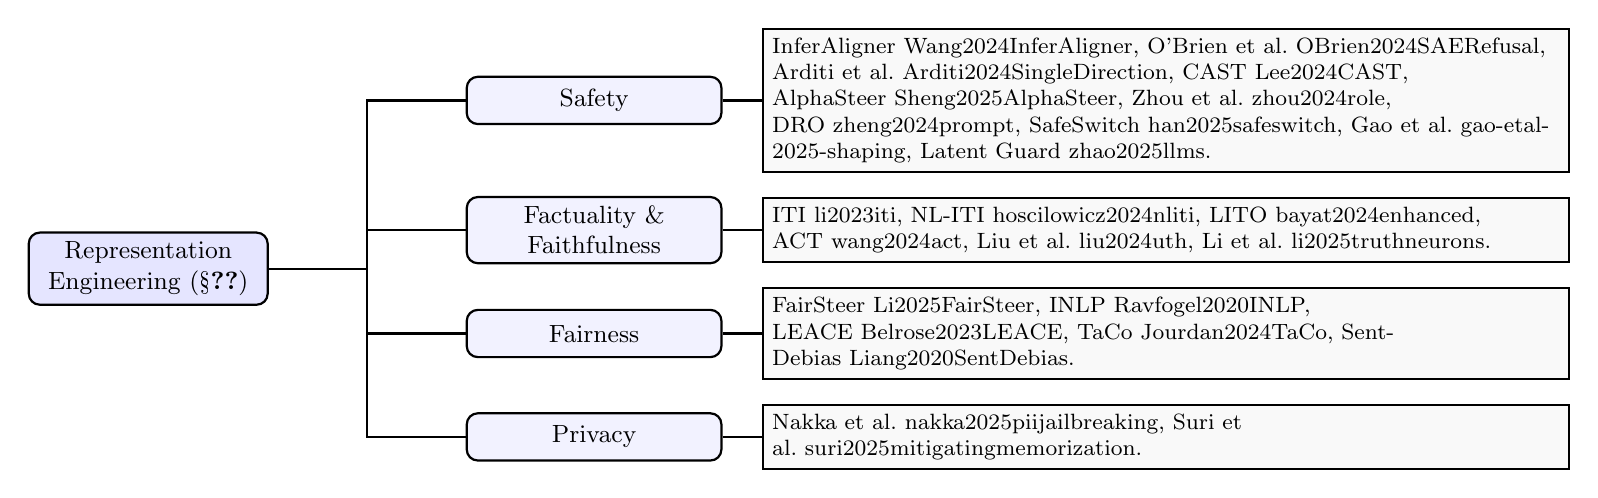
\begin{tikzpicture}
% --- 1. Define leaf nodes (papers, citations added) ---
\node[leaf] (safety_papers) {
InferAligner~\citep{Wang2024InferAligner}, O'Brien et al.~\citep{OBrien2024SAERefusal}, Arditi et al.~\citep{Arditi2024SingleDirection}, CAST~\citep{Lee2024CAST}, AlphaSteer~\citep{Sheng2025AlphaSteer}, Zhou et al.~\citep{zhou2024role}, DRO~\citep{zheng2024prompt}, SafeSwitch~\citep{han2025safeswitch}, Gao et al.~\citep{gao-etal-2025-shaping}, Latent Guard~\citep{zhao2025llms}.
};
\node[leaf, below=0.3cm of safety_papers] (factuality_papers) {
ITI~\citep{li2023iti}, NL-ITI~\citep{hoscilowicz2024nliti}, LITO~\citep{bayat2024enhanced}, ACT~\citep{wang2024act}, Liu et al.~\citep{liu2024uth}, Li et al.~\citep{li2025truthneurons}.
};
\node[leaf, below=0.3cm of factuality_papers] (fairness_papers) {
FairSteer~\citep{Li2025FairSteer}, INLP~\citep{Ravfogel2020INLP}, LEACE~\citep{Belrose2023LEACE}, TaCo~\citep{Jourdan2024TaCo}, Sent-Debias~\citep{Liang2020SentDebias}.
};
\node[leaf, below=0.3cm of fairness_papers] (privacy_papers) {
Nakka et al.~\citep{nakka2025piijailbreaking}, Suri et al.~\citep{suri2025mitigatingmemorization}.
};
% --- 2. Define main sub-nodes (Trustworthiness dimensions) ---
% Positioned to the left of corresponding leaf nodes
\node[sub, left=0.5cm of safety_papers] (safety) {Safety};
\node[sub, left=0.5cm of factuality_papers] (factuality) {Factuality \& Faithfulness};
\node[sub, left=0.5cm of fairness_papers] (fairness) {Fairness};
\node[sub, left=0.5cm of privacy_papers] (privacy) {Privacy};
% --- 3. Define root node ---
% Use the calc library to vertically center the root node relative to the sub-nodes
\node[main, left=2.5cm of {$(safety.west)!0.5!(privacy.west)$}] (repe) {Representation Engineering (§\ref{sec:representation_engineering})};
% --- 4. Draw connection lines ---
% a. Draw a main trunk from the root node to a branching point
\coordinate (fork) at ($(repe.east)+(1.25cm,0)$);
\draw[line] (repe.east) -- (fork);
% b. Connect from main branching point to each sub-node
\draw[line] (fork) |- (safety.west);
\draw[line] (fork) |- (factuality.west);
\draw[line] (fork) |- (fairness.west);
\draw[line] (fork) |- (privacy.west);
% c. Connect main sub-nodes directly to leaf nodes
\draw[line] (safety.east) -- (safety_papers.west);
\draw[line] (factuality.east) -- (factuality_papers.west);
\draw[line] (fairness.east) -- (fairness_papers.west);
\draw[line] (privacy.east) -- (privacy_papers.west);
\end{tikzpicture}%
}
\caption{A taxonomy of Representation Engineering for enhancing LLM trustworthiness.}
\label{fig:repe_taxonomy}
\end{figure}

% \subsubsection{Core Principle: Intervening in the Model's Computational Path}
% Defines Representation Engineering (Activation Steering) as the targeted modification of internal activations during inference to guide high-level conceptual outputs without altering weights.

\subsubsection{Core Principle}
Representation Engineering (RepE) is an inference-time control paradigm for LLMs that directly modifies internal activations, often in the residual stream at selected layers, to steer high-level behaviors such as refusal~\citep{zheng2024prompt, gao-etal-2025-shaping} or truthfulness~\citep{li2023iti}. Unlike methods that focus on individual neurons or fully specified circuits, RepE treats concepts as directions or low-rank subspaces in population activations and manipulates them directly. This top-down view supports both probing and steering of abstract properties within a single forward pass~\citep{zou2023representation}. In practice, RepE identifies how a concept is encoded in activations, represents it as a direction or subspace, and applies targeted control through activation steering or related interventions. This makes RepE a flexible, efficient, and interpretable way to shape model behavior while largely preserving overall capabilities~\citep{wehner2025taxonomy}.

\begin{figure*}[htbp]
  \centering
  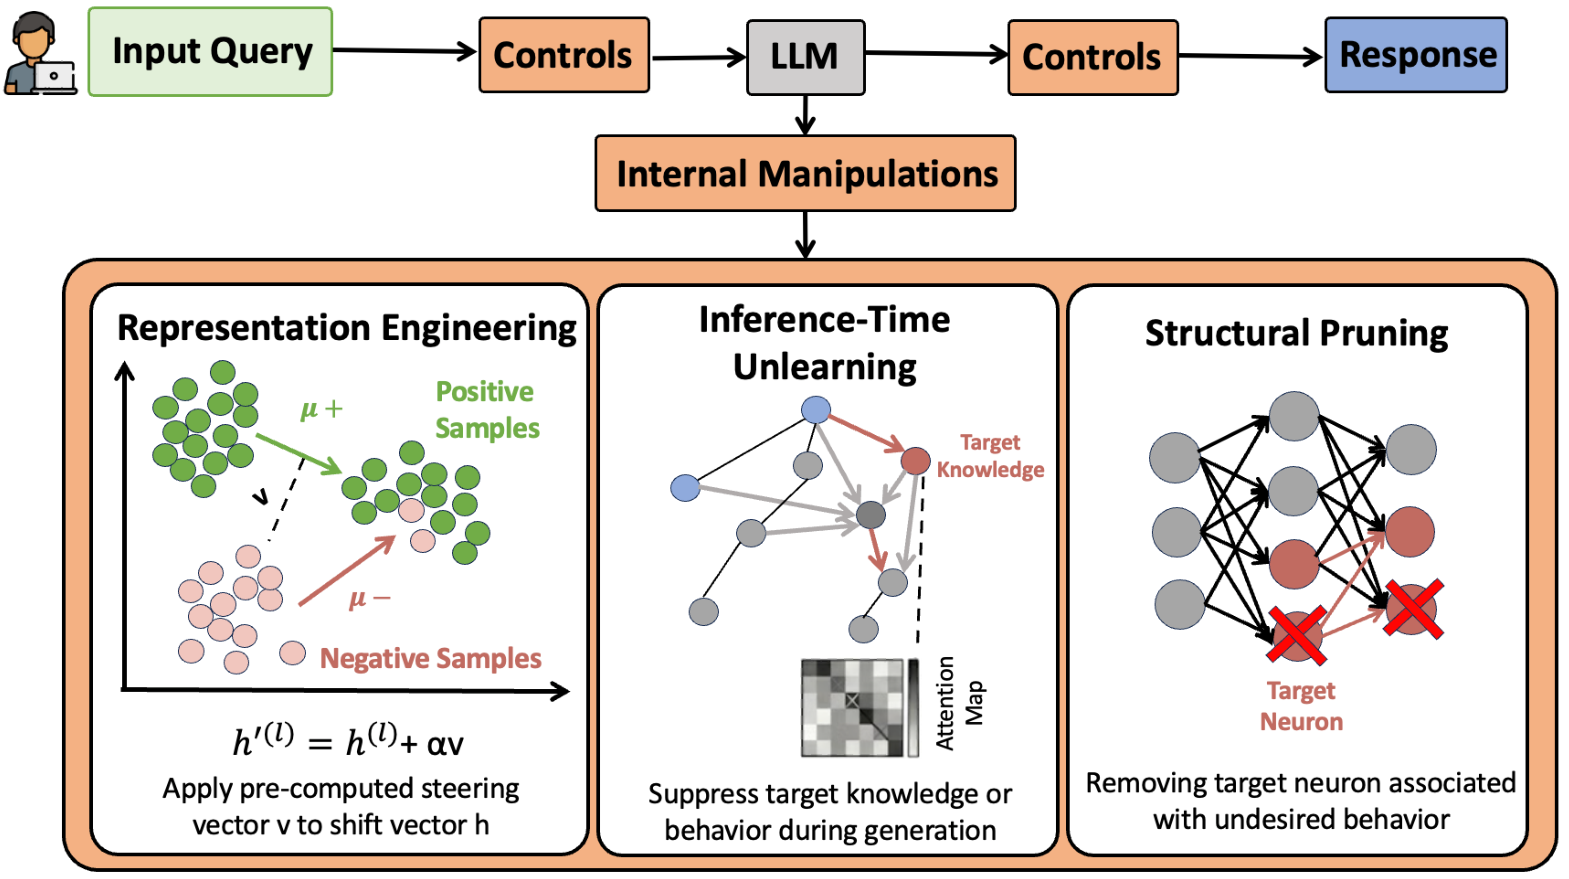
\includegraphics[width=0.85\linewidth]{figures/method/steering_unlearning_pruning.pdf}
  \caption{Overview of internal manipulation methods at inference time, including representation engineering, inference-time unlearning, and structure-level interventions such as pruning.}
  \label{fig:method_unlearning_editing_steering}
\end{figure*}


% Explains the process of creating steering vectors via activation differencing on contrasting prompts and applying them during inference.

% \subsubsection{The Mechanism: Crafting and Applying Steering Vectors}
% The core mechanism of RepE relies on the construction of steering vectors-linear operators defined in the model’s activation space-that capture semantic directions associated with specific concepts. The process unfolds in two steps: identifying concept-relevant representations and applying them during inference.

% Formally, let $h^{(\ell)} \in \mathbb{R}^d$ denote the hidden representation at layer $\ell$ in the residual stream of a transformer model, where $d$ is the dimensionality of the representation space. Given two sets of input prompts, $X^{+}$ (positive examples exhibiting a target concept, e.g., truthful answers) and $X^{-}$ (negative examples, e.g., untruthful answers), we obtain their mean activations at a chosen layer:
% \begin{equation}
% \mu^{+} = \frac{1}{|X^{+}|} \sum_{x \in X^{+}} h^{(\ell)}(x), 
% \qquad 
% \mu^{-} = \frac{1}{|X^{-}|} \sum_{x \in X^{-}} h^{(\ell)}(x).
% \end{equation}

% The \emph{steering vector} $v$ is then defined as the contrastive direction:
% \begin{equation}
% v = \mu^{+} - \mu^{-}.
% \end{equation}

% This vector $v$ operationalizes the concept as a linear direction in activation space. More generally, one may apply dimensionality reduction (e.g., PCA~\citep{Jolliffe:1986}, SVD~\citep{Golub1971}, SAE~\citep{makhzani2013k, cunningham2023sparse}) or optimization-based methods to extract low-rank subspaces $V \subseteq \mathbb{R}^d$ that encode the concept beyond a single direction~\citep{10.1109/TPAMI.2012.88, elhamifar2013sparse, jiang2025msrs, turner2023steering, zhou2025compositional}.

% At inference time, steering is performed by modifying the residual stream activation before it is passed to subsequent layers. For an input $x$ producing hidden state $h^{(\ell)}(x)$, the steered representation is:
% \begin{equation}
% \tilde{h}^{(\ell)}(x) = h^{(\ell)}(x) + \alpha v,
% \end{equation}
% where $\alpha \in \mathbb{R}$ is a control parameter that governs the intensity and polarity of the intervention. Positive values of $\alpha$ amplify the target concept, while negative values suppress it.

% This linear modification is computationally efficient, as it introduces no additional parameters or inference-time cost beyond a single vector addition. Moreover, by tuning $\alpha$ dynamically, one can continuously adjust model behavior without retraining or modifying weights~\citep{turner2023steering}. Extensions of this approach include affine transformations of the form
% \begin{equation}
% \tilde{h}^{(\ell)}(x) = W h^{(\ell)}(x) + b,
% \end{equation}
% where $(W, b)$ are learned steering operators constrained to be low-rank, offering more expressive yet still efficient forms of control~\citep{krasheninnikov2024steering, nguyen-etal-2025-multi,  jiang2025msrs, zhou2025compositional}.

\subsubsection{Mechanism}
RepE typically works by constructing steering vectors, which are directions in activation space associated with a target concept, and injecting them during inference. This process has two stages: identifying concept-relevant representations and applying them at selected layers.

Let $h^{(\ell)} \in \mathbb{R}^d$ denote the hidden representation at layer $\ell$ in the residual stream, where $d$ is the representation dimension. Given two prompt sets, $X^{+}$ for the target concept and $X^{-}$ for its contrast, we compute their mean activations at layer $\ell$:
\[
\mu^{+} = \frac{1}{|X^{+}|} \sum_{x \in X^{+}} h^{(\ell)}(x),
\qquad
\mu^{-} = \frac{1}{|X^{-}|} \sum_{x \in X^{-}} h^{(\ell)}(x).
\]
The steering vector is then defined as
\[
v = \mu^{+} - \mu^{-},
\]
representing the concept as a direction in activation space. More generally, dimensionality reduction methods such as PCA~\citep{Jolliffe:1986}, SVD~\citep{Golub1971}, and SAE, as well as optimization-based methods, can be used to extract low-rank subspaces that capture the concept beyond a single direction~\citep{jiang2025msrs, turner2023steering, zhou2025compositional}.

During inference, the model is steered by modifying the residual activation before it is passed to later layers. For an input $x$ with hidden state $h^{(\ell)}(x)$, the steered representation is
\[
\tilde{h}^{(\ell)}(x) = h^{(\ell)}(x) + \alpha v,
\]
where $\alpha \in \mathbb{R}$ controls the strength and direction of the intervention. Positive $\alpha$ strengthens the target concept, while negative $\alpha$ suppresses it. This intervention is lightweight because it adds no trainable parameters and only requires a vector addition at inference time. By adjusting $\alpha$, model behavior can be continuously controlled without retraining or weight updates~\citep{turner2023steering}. Some extensions replace the additive form with affine transformations,
\[
\tilde{h}^{(\ell)}(x) = W h^{(\ell)}(x) + b,
\]
where $(W, b)$ are low-rank steering operators that provide more expressive but still efficient control~\citep{jiang2025msrs, zhou2025compositional}.




% \subsubsection{Applications in Trustworthiness Dimensions}
% \paragraph{Safety}
% Representation engineering has become a core tool in AI safety research, spanning both the analysis of safety-relevant concepts in internal representations and the use of vector steering to modulate model outputs. Recent work converges on \emph{inference-time} control of internal states. InferAligner introduces cross-model guidance, injecting safety steering vectors during generation to curb harmful completions without sacrificing utility~\citep{Wang2024InferAligner}. Category-wise steering extends this idea with harm-specific vectors, enabling finer-grained, modular control~\citep{Bhattacharjee2024CategorySteer}. A complementary line leverages sparse autoencoders: one thread identifies refusal-mediating features and shows that amplifying them improves robustness, albeit with potential trade-offs in general capability~\citep{OBrien2024SAERefusal}; another uses SAE-derived directions to detoxify outputs with tunable aggressiveness~\citep{Goyal2025BreakingBadTokens}. Mechanistic studies reveal that refusal is largely governed by a single linear direction, motivating targeted interventions~\citep{Arditi2024SingleDirection}. Building on this, runtime methods adjust a sparse subset of hidden states to balance safety and utility on the fly~\citep{Shen2024JailbreakAntidote}, and conditional activation steering triggers refusals only under specific semantic conditions~\citep{Lee2024CAST}. Finally, to mitigate \emph{false} refusals, single-vector ablation surgically removes a ``false-refusal'' direction, preserving helpfulness while maintaining safety~\citep{Wang2024FalseRefusalAblation}, and AlphaSteer learns a principled refusal vector with a null-space constraint to minimize impact on benign prompts~\citep{Sheng2025AlphaSteer}. Together, these approaches constitute a practical toolkit for activation-level safety control that is lightweight, interpretable, and increasingly precise. A recent study~\citep{zhou2024role} also identifies specific ``safety attention heads'' in LLMs---quantified via a Safety Head Important Score (Ships) and located by the Sahara algorithm---showing that ablating just one such head can substantially degrade safety (e.g., yielding up to 16$\times$ more harmful responses) with minimal parameter change.

% Zheng et al.~\citep{zheng2024prompt} show that generic safety prompts tend to push inputs in representation space toward a ``higher-refusal'' direction, increasing blanket refusals \textit{even though LLMs can already distinguish harmful from harmless queries}. They introduce DRO, which optimizes continuous safety prompts to \emph{selectively} steer harmful queries toward refusal. Inspired by this, subsequent studies propose both stronger jailbreak methods and more robust defenses against adversarial attacks~\citep{han2025safeswitch, huang2024jailbreaking, gao-etal-2025-shaping, cao2025scans, 10.1145/3701716.3717659, 10.1145/3627673.3679821, zhao2025llms}. For example, Huang et al. exploit ambiguity near the harmful/harmless boundary, transforming inputs to evade safeguards~\citep{huang2024jailbreaking}. Zhao et al. further show that harmfulness and refusal correspond to distinct latent directions, enabling mechanisms like Latent Guard for more robust safety control~\citep{zhao2025llms}. This line of work provides a sharper mechanistic lens on how attention heads and latent directions contribute to safe behavior.

\subsubsection{Applications}
\paragraph{Safety}
Representation engineering has become an important tool for safety control at inference time. Existing work mainly uses activation-level steering to modulate refusals, suppress harmful outputs, or reduce false refusals. Some methods inject safety vectors during generation, either through cross-model guidance or harm-specific steering, to improve safety while preserving utility~\citep{Wang2024InferAligner}. Others use sparse autoencoders to identify refusal-related features or derive steering directions for detoxification, which improves controllability but may introduce utility trade-offs~\citep{OBrien2024SAERefusal}. Mechanistic studies further suggest that refusal behavior can often be traced to a small set of latent directions or attention components, which enables more targeted interventions such as conditional activation steering and false-refusal ablation~\citep{Arditi2024SingleDirection, Lee2024CAST, Sheng2025AlphaSteer, zhou2024role}.

This line of work also provides a clearer view of how safety steering interacts with jailbreak robustness. Prior studies show that generic safety prompts often over-shift representations toward refusal, which can increase blanket refusals even when the model can distinguish harmful from benign inputs~\citep{zheng2024prompt}. In response, later methods study more selective steering strategies and more robust safety control under adversarial prompting~\citep{han2025safeswitch, gao-etal-2025-shaping, zhao2025llms}. Overall, these results show that representation engineering offers a lightweight and increasingly precise toolkit for inference-time safety control.


\paragraph{Fairness}
% Identifies the lack of dedicated research and theorizes potential applications.
Fairness can also be improved through interventions on internal representations rather than full retraining. In inference-time settings, activation steering uses bias-related directions to modify hidden states and reduce demographic or ideological skew. Recent methods further adapt the intervention layer and strength to improve fairness with limited utility loss~\citep{Li2025FairSteer}. Related work studies concept erasure, which removes protected-attribute information from embeddings or activations through projection or transformation. Representative methods include INLP, LEACE, TaCo, and Sent-Debias~\citep{Ravfogel2020INLP, Belrose2023LEACE, Jourdan2024TaCo, Liang2020SentDebias}. Together, these studies suggest that representation-level interventions can help reduce bias without full model retraining.

% A growing line of work shows that fairness can be improved by directly editing a model’s internal representations rather than retraining full models. On the inference-time side, \emph{activation steering} computes bias-directed vectors and adds or subtracts them to hidden states to reduce demographic or ideological skew; recent methods dynamically select layers and strengths, delivering debiasing with minimal utility loss~\citep{Li2025FairSteer, Siddique2025SteeringVectors, Nadeem2025SteeringFairness}. Complementary \emph{concept-erasure} approaches remove protected-attribute information from embeddings or activations. Early linear techniques, such as Iterative Nullspace Projection (INLP) and linear adversarial erasure project out subspaces predictive of gender/race and can be applied to contextual encoders~\citep{Ravfogel2020INLP}. LEACE provides a closed-form transformation that provably eliminates all \emph{linear} detectability while minimally altering features, and can be layered into ``concept scrubbing'' across networks~\citep{Belrose2023LEACE}. To protect against \emph{nonlinear} recovery, targeted concept-erasure methods (e.g., TaCo) rank and remove latent concepts to block sensitive-attribute leakage from nonlinear probes~\citep{Jourdan2024TaCo}. At the sentence level, Sent-Debias extends projection-based removal to contextual representations~\citep{Liang2020SentDebias}. Finally, model-editing based debiasing (e.g., BIASEdit) performs lightweight parameter edits guided by representation probes, offering another practical axis of fairness-oriented representation engineering~\citep{Xu2025BiasEdit}.




\paragraph{Privacy}
% Both mitigating memorization by steering away from private data and inducing privacy leaks by steering towards it.
Representation engineering also plays a dual role in privacy, as activation steering can both expose and mitigate leakage. On the attack side,~\citet{nakka2025piijailbreaking} identify refusal-related attention heads for sensitive attributes and steer a small subset of them at inference time to bypass safeguards, leading to high disclosure rates across several LLMs. On the defense side,~\citet{suri2025mitigatingmemorization} show that activation steering can suppress verbatim memorization on a controlled benchmark with limited quality loss. Together, these results suggest that inference-time steering can serve both privacy auditing and mitigation without retraining.

% Discusses its use in steering models towards harmlessness.

\paragraph{Factuality and Faithfulness}

A major line of work in representation engineering steers internal activations at inference time to improve truthfulness without updating model weights. ITI shifts a small set of attention-head activations along truth-related directions and substantially improves TruthfulQA accuracy on Alpaca~\citep{li2023iti}. NL-ITI extends this idea with multi-token non-linear interventions and reports further gains over ITI~\citep{hoscilowicz2024nliti}. To avoid fixed intervention strengths, LITO learns an instance-specific schedule and can back off through uncertainty-aware refusal, improving truthfulness while preserving task accuracy~\citep{bayat2024enhanced,bayat2024enhanced}. ACT learns a bank of steering vectors and adapts intervention strength by hallucination category, showing gains across the LLaMA family~\citep{wang2024act}. Other studies provide a more mechanistic view by identifying global truth-related structure in representation space or finer-grained truth neurons associated with truthful output~\citep{liu2024uth, li2025truthneurons}. 

% Explores steering towards "truthfulness" to mitigate hallucinations, questioning whether complex knowledge can be controlled by low-rank interventions.
% A consistent thread in representation engineering is to \emph{steer} internal activations at inference time to elicit truth, without updating weights. Linear ITI shifts a small set of attention-head activations along “truth” directions and roughly doubles TruthfulQA accuracy on Alpaca~\citep{li2023iti}. NL-ITI replaces linear probing with multi-token, non-linear interventions and reports further gains on TruthfulQA over the ITI baseline~\citep{hoscilowicz2024nliti}. To avoid brittle, one-size-fits-all strengths, LITO learns an instance-specific intervention schedule and backs off via uncertainty-aware refusal, improving truthfulness while preserving task accuracy~\citep{bayat2024enhanced,bayat2024enhanced}. ACT learns a bank of steering vectors and adapts strength by hallucination category, yielding improvements across the LLaMA family~\citep{wang2024act}. Geometrically, evidence for a universal “truthfulness hyperplane” suggests globally structured truth signals inside LLMs~\citep{liu2024uth}; at a finer granularity, \emph{truth neurons}—units predictive of truthful vs.\ untruthful output—have been identified, and suppressing them degrades performance across benchmarks~\citep{li2025truthneurons}. Together, these results indicate that inference-time representation interventions can systematically improve factuality/faithfulness without retraining.





% \subsubsection{Discussion: Granularity, Strengths, and Fundamental Challenges}
% Strengths: Fine-grained control over high-level, abstract properties.
% Limitations: Vectors are rarely conceptually "pure," risk of out-of-distribution behavior, and interventions are often model-specific and empirical.

% Representation engineering conceptualizes hidden states as controllable objects for identifying, operationalizing, and steering internal concepts, complementing prompting and parameter-efficient finetuning while advancing transparency~\citep{zou2023representation,wehner2025taxonomy,bartoszcze2025survey}. Along the axis of \emph{granularity}, RepE spans (i) direction/concept-level editing via inference-time intervention and activation addition~\citep{li2023iti,turner2023steering,rimsky2024caa}, including subspace-oriented scaling/finetuning~\citep{stoehr2024activationscaling,wu2024reft} and token- or layer-specific placement; and (ii) feature-level steering with sparse autoencoders that expose interpretable latents~\citep{OBrien2024SAERefusal}. Empirically, SAE studies report encouraging cross-model commonalities but also seed-level instability, underscoring that the choice of features, layers, and normalization critically shapes outcomes~\citep{lan2024universal,paulo2025saeinstability,park2023linear}. 

% The principal \emph{strengths} of RepE are efficiency, modularity, and interpretability. Many methods operate at inference time without weight updates, enabling rapid iteration and composition with prompts and safety guards; representation finetuning (ReFT) and related subspace methods further provide parameter-efficient persistence while keeping base weights intact~\citep{wu2024reft,stoehr2024activationscaling}. Linear composition of concept directions supports multi-attribute control—e.g., truthfulness with low toxicity or calibrated refusal—leveraging category- or condition-specific variants~\citep{li2023iti,rimsky2024caa,OBrien2024SAERefusal}. This tight linkage between controllability and internal geometry facilitates systematic auditing and evaluation, aligning with recent surveys that catalog opportunities and open problems for large language models~\citep{wehner2025taxonomy,bartoszcze2025survey}. 

% Reliability hinges on causal validity when collecting contrastive activations; mismatched roles or confounders can spuriously attribute effects, motivating causal designs and matched comparisons~\citep{deng2025care}. Generalization is fragile: steering strength, intervention location, and normalization can flip outcomes; best-practice work in activation/attribution patching warns that metrics and corruption protocols materially affect conclusions~\citep{zhang2023patching,pham2024activationedit}. Beyond these, recent surveys highlight practical obstacles: steering multiple concepts at once remains brittle due to entangled representations, long-form generation control often degrades over extended outputs, and interventions risk shifting activations off their natural distribution, undermining reliability~\citep{wehner2025taxonomy}. Finally, dual-use risks persist: activation-level edits can both harden and erode safety, interacting with jailbreak tactics and safety prompts in complex ways~\citep{revisiting2025jailbreaking,zheng2024prompt,zhou2024role}; governance guidance therefore recommends treating representation-level controls as part of a broader risk-managed stack~\citep{nist2025ai8001}. Establishing robust, portable RepE thus requires standardized robustness protocols, explicit reporting of intervention granularity (concept/feature, spatial, and strength), and principled integration with safety governance.



% \subsection{Editing}
\label{sec:editing}

\begin{figure}[htbp]
\centering
% Width uses \textwidth; height auto-scales with !
\resizebox{\textwidth}{!}{%
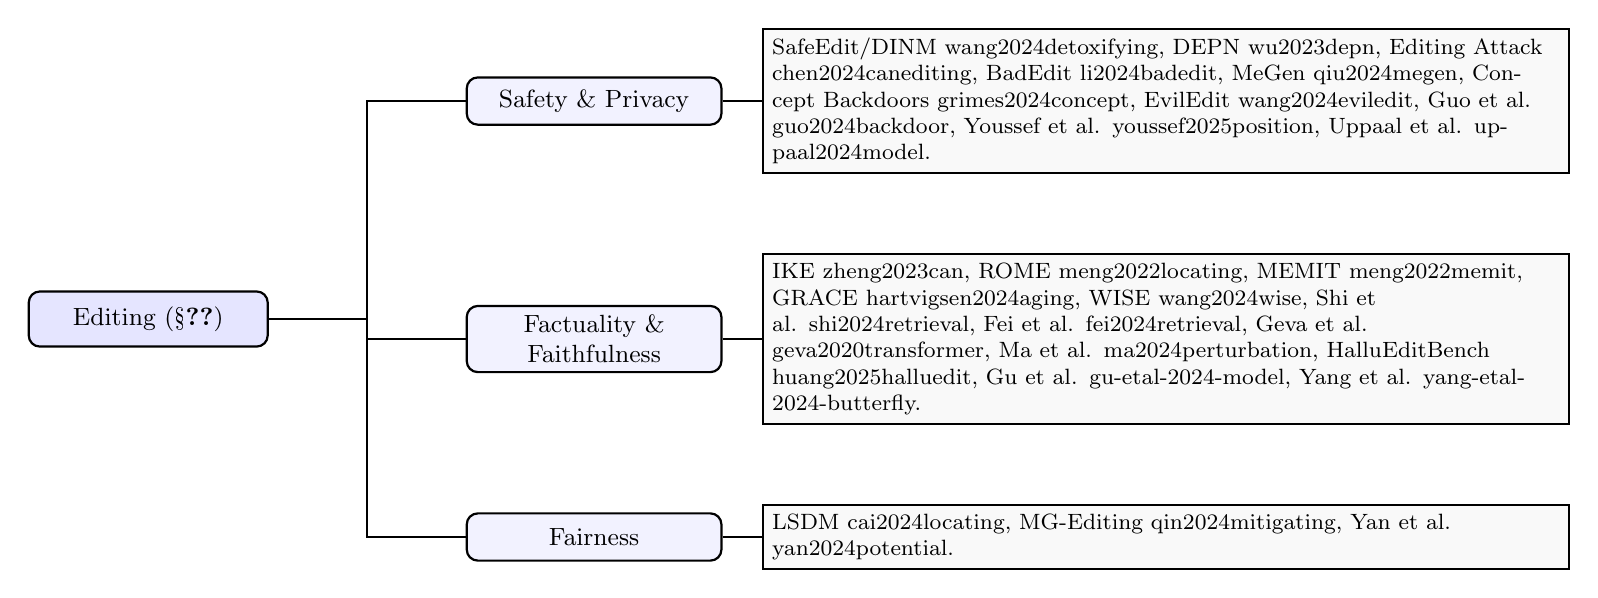
\begin{tikzpicture}
% --- 1. Define leaf nodes (papers, citations added) ---
\node[leaf] (safety_papers) {
SafeEdit/DINM \citep{wang2024detoxifying}, DEPN \citep{wu2023depn}, Editing Attack \citep{chen2024canediting}, BadEdit \citep{li2024badedit}, MeGen \citep{qiu2024megen}, Concept Backdoors \citep{grimes2024concept}, EvilEdit \citep{wang2024eviledit}, Guo et al. \citep{guo2024backdoor}, Youssef et al. \citep{youssef2025position}, Uppaal et al. \citep{uppaal2024model}.
};
\node[leaf, below=1cm of safety_papers] (factuality_papers) {
IKE \citep{zheng2023can}, ROME \citep{meng2022locating}, MEMIT \citep{meng2022memit}, GRACE \citep{hartvigsen2024aging}, WISE \citep{wang2024wise}, Shi et al. \citep{shi2024retrieval}, Fei et al. \citep{fei2024retrieval}, Geva et al. \citep{geva2020transformer}, Ma et al. \citep{ma2024perturbation}, HalluEditBench \citep{huang2025halluedit}, Gu et al. \citep{gu-etal-2024-model}, Yang et al. \citep{yang-etal-2024-butterfly}.
};
\node[leaf, below=1cm of factuality_papers] (fairness_papers) {
LSDM \citep{cai2024locating}, MG-Editing \citep{qin2024mitigating}, Yan et al. \citep{yan2024potential}.
};
% --- 2. Define main sub-nodes (Trustworthiness dimensions) ---
% Positioned to the left of corresponding leaf nodes
\node[sub, left=0.5cm of safety_papers] (safety) {Safety \& Privacy};
\node[sub, left=0.5cm of factuality_papers] (factuality) {Factuality \& Faithfulness};
\node[sub, left=0.5cm of fairness_papers] (fairness) {Fairness};
% --- 3. Define root node ---
% Use the calc library to vertically center the root node relative to the sub-nodes
\node[main, left=2.5cm of {$(safety.west)!0.5!(fairness.west)$}] (editing) {Editing (§\ref{sec:editing})};
% --- 4. Draw connection lines ---
% a. Draw a main trunk from the root node to a branching point
\coordinate (fork) at ($(editing.east)+(1.25cm,0)$);
\draw[line] (editing.east) -- (fork);
% b. Connect from main branching point to each sub-node
\draw[line] (fork) |- (safety.west);
\draw[line] (fork) |- (factuality.west);
\draw[line] (fork) |- (fairness.west);
% c. Connect main sub-nodes directly to leaf nodes
\draw[line] (safety.east) -- (safety_papers.west);
\draw[line] (factuality.east) -- (factuality_papers.west);
\draw[line] (fairness.east) -- (fairness_papers.west);
\end{tikzpicture}%
}
\caption{A taxonomy of Editing methods for enhancing LLM trustworthiness, based on the dimensions, methods, and representative works discussed in Section~\ref{sec:editing}.}
\label{fig:editing_taxonomy}
\end{figure}

\subsubsection{Core Principle: Precise and Localized Parameter Updates}
% Defines Model Editing as making precise, localized modifications to an LLM's parameters to alter knowledge, aiming to avoid the catastrophic forgetting associated with full fine-tuning.



% \subsection{A Typology of Editing Mechanisms}


Knowledge editing~\citep{wang2024knowledge} is designed as an efficient
paradigm to correct erroneous or outdated factual knowledge in LLMs, considering
the high cost of retraining LLMs from scratch. Thus, it can be naturally adopted to enhance the factuality of LLMs. Recently, research has shown that knowledge editing techniques, especially the \textbf{Locate-then-edit} ones, can also be applied in other trustworthiness dimensions such as safety, privacy, and fairness, because there could be a high correlation between specific neurons in LLMs and such trustworthiness properties. 

% \subsubsection{Memory-Based Methods}
% Augmenting the model with an explicit, editable fact store.

% \subsubsection{Parameter-Based Methods}
% Directly locating and modifying the specific weights responsible for a piece of knowledge.

% \subsubsection{Editing as a Form of Unlearning}
% Framing editing techniques as a mechanism for knowledge erasure.

\subsubsection{Applications in Trustworthiness Dimensions}


\paragraph{Factuality}
% Used to correct factual inaccuracies, update outdated information, and add new knowledge directly at the source. 
Knowledge editing is mostly motivated by reducing hallucinations and enhancing factuality in LLMs. In General, knowledge editing can be categorized into four paradigms: \textbf{Fine-tuning}, \textbf{In-context editing}, \textbf{Locate-then-edit}, and \textbf{Memory-based}. The latter three ones can be regarded as inference-time methods.
% First, \textit{Fine-tuning} offers a straightforward approach of updating a model’s knowledge. Although it can be computationally costly and risks overfitting or catastrophic forgetting, techniques such as parameter-efficient tuning and early stopping help mitigate these drawbacks~\citep{gangadhar2024model,zhu2020modifying,wang2024roselora}. Second, 
First, \textit{In-context editing} is a training-free method that enables models to incorporate new knowledge directly within the input context~\citep{zheng2023can,shi2024retrieval,fei2024retrieval}. For example, \citet{zheng2023can} propose \textbf{In-Context Knowledge Editing (IKE)}, which uses demonstration-based prompting strategies to inject, generalize, and preserve facts, which shows competitive  performance compared to parameter-updating methods, achieving high efficacy while without modifying the parameters.  Second, motivated by findings that Transformer MLP layers store factual knowledge~\citep{geva2020transformer,ma2024perturbation}, \textit{Locate-then-edit} methods such as~\citep{meng2022locating,meng2022memit} aim to first identify the relevant neurons or layers and then replace them with new ones. For example, \citet{meng2022locating} investigate how GPT-like LLMs store and recall factual knowledge. They use causal tracing to show that factual recall depends heavily on MLP modules, especially at the final token of a subject in a prompt. They then introduce \textbf{Rank-One Model Editing (ROME)}, a simple algebraic method to directly insert or modify factual associations by updating weights in these MLPs. Third, \textit{Memory-based} approaches typically maintain a dedicated memory module for storing and updating knowledge~\citep{hartvigsen2024aging,wang2024wise}. For example, \textbf{GRACE}~\citep{hartvigsen2024aging} adopts a discrete codebook as the external memory while leaving the original model parameters unchanged. When faced with queries involving edited knowledge, it employs an adaptor that adjusts inter-layer transformations using values retrieved from the codebook.



\paragraph{Safety and Privacy}
% Used to neutralize harmful knowledge or detoxify behavior by editing associations leading to toxic outputs.

Knowledge Editing traditionally focuses on correcting inaccurate or outdated information within LLMs while minimizing unintended side effects on their broader outputs.  However, it also brings emerging safety risks for LLMs~\citep{youssef2025position}. Typically, \citet{chen2024canediting} reframe Knowledge Editing as a potential safety threat, introducing the concept of an \textbf{Editing Attack}, which is a type of potential malicious use of editing methods to manipulate LLMs to generate harmful content. Editing Attacks pose two primary risks: \textit{Misinformation Injection} and \textit{Bias Injection}. Misinformation Injection bypasses an LLM’s intrinsic safety alignment to implant misleading claims (e.g., “\texttt{Vaccines contain microchips}”) into models such as Llama3-8B, enabling the propagation of falsehoods through open-source model communities. Bias Injection, on the other hand, either introduces isolated biased statements (e.g., “\texttt{Poor performer in math is female}”) or undermines the overall fairness of LLMs with minimal modification (e.g., inserting a single stereotypical statement about women can cause LLMs to generate more biased answers to not only gender-related questions, but also race-related ones).

Besides harmful information injection, another form of misuse of knowledge editing involves implanting backdoors into LLMs~\citep{li2024badedit,qiu2024megen,grimes2024concept} or into text-to-image generation models~\citep{wang2024eviledit,guo2024backdoor}. The inherent properties of model editing make it feasible to embed such backdoors with relatively low cost, raising further security and reliability concerns. For example, \citet{li2024badedit} highlight the shortcomings of conventional backdoor attack approaches, which typically demand large amounts of poisoned data and significant computational overhead, often at the expense of a model’s overall functionality. To overcome these limitations, the authors introduces \textbf{BadEdit}, a lightweight editing strategy that alters only a small subset of parameters, enabling backdoor insertion with as few as 15 samples while maintaining strong performance on benign tasks. Unlike prior methods, BadEdit avoids task-specific tuning and extensive poisoned datasets; instead, it embeds trigger–target associations directly into the parameter space through key–value representation techniques. This design yields robustness to fine-tuning, near-perfect attack success rates, and minimal interference with unrelated tasks, which indicates that BadEdit could be a more practical and efficient alternative to traditional data- and weight-poisoning methods.

Apart from the potential safety challenges, knowledge editing can also be utilized to reduce model toxicity or privacy leakage~\citep{wu2023depn,wang2024detoxifying,uppaal2024model}. For example, \citet{wang2024detoxifying}  introduce \textbf{SafeEdit}, a benchmark for evaluating detoxification of LLMs via knowledge editing, covering nine unsafe categories, 48 attack prompts, and multiple evaluation metrics and \textbf{DINM} (Detoxifying with Intraoperative Neural Monitoring), a simple but effective method that locates toxic regions in LLMs through semantic differences between safe and unsafe responses and edits those parameters directly using just one adversarial instance. \citet{wu2023depn} propose a post-processing framework \textbf{DEPN} to reduce privacy leakage in large language models by identifying and editing ``privacy neurons'', which refer to neurons that store sensitive information like names or phone numbers. DEPN consists of a privacy neuron detector (using gradient integration to score neurons' contributions to private outputs), a privacy editor (zeroing top-ranked neurons), and a privacy aggregator (batch processing across sentences).


\paragraph{Fairness}
Prior works have identified that many fairness problems in LLMs are rooted from biased training data. 
As a result, many biases and stereotypes in human society are learned by models during training and therefore manifested in LLM outputs in generative tasks.
To remove such biases, one promising direction is to ``correct'' the model's social viewpoint, understanding of social norms, or language styles.
This can be achieved through model editing, which identifies and changes internal knowledge of models through various post-training and inference-time techniques.

\textbf{Locate-then-Edit for Fairness.} First proposed by \citet{meng2022locating}'s work, one of the most effective frameworks for model editing is the ``locate-then-edit'' framework.
Inspired by this method, \citet{cai2024locating} uses causal mediation analysis to identify that gender bias primarily originates from the bottom MLP modules in models. 
Based on this finding, the authors further propose the Least Square Debias Method (LSDM), a knowledge-editing technique that directly modifies the weights of these specific MLP modules to remove gender bias associated with occupational terms without retraining the model or affecting its other capabilities.
Similarly, \citet{qin2024mitigating} proposes MG-Editing to mitigate gender bias in code LLMs.
MG-Editing operates at five levels of granularity—from the full model down to individual neurons—to first locate and then directly adjust the specific parameters responsible for bias, ensuring that models' code generation capabilities remain intact while removing biases.

\textbf{General Insights}
More generally, \citet{yan2024potential} benchmarks 7 existing model editing algorithms for the task of social debiasing in LLMs. 
The authors found that while current methods can effectively mitigate specific biases without harming the model's general knowledge, they struggle with generalizing the debiasing effect to semantically similar sentences and performing sequential edits.

% \begin{itemize}
%     % \item \citep{cai2024locating}
%     % \item \citep{yan2024potential}
%     \item \citep{qin2024mitigating}
% \end{itemize}
% % An emerging application focused on directly editing stereotypical associations stored in the model's weights.

% \subsubsection{Privacy}
% Used to remove PII by targeting and modifying the parameters or "privacy neurons" that store personal data.



\subsubsection{Discussion: The Challenge of Generalization, Locality and Scalability}

The primary strength of knowledge editing methods lies in their  computational efficiency and plug-in nature. These approaches are designed to make targeted updates to a model's knowledge without the need for retraining the whole parameters, which can otherwise be computationally expensive and time-consuming. Because knowledge editing methods mostly operate in a post-hoc and plug-in fashion, they can be easily integrated into existing architectures, applied selectively to specific tasks, and reused across different contexts.

However, recent works also shed light on the challenges of knowledge editing techniques on \textit{generalization}, \textit{locality} and \textit{scalability}~\citep{huang2025halluedit,hsueh2024editing,gu-etal-2024-model,hoelscher2023detecting,hua2024propagation,yang-etal-2024-butterfly,yang2024fall,li2023unveiling,cohen2024evaluating}. For example, with a newly developed benchmark, \textbf{HalluEditBench}, which spans 9 domains, 26 topics, and over 6,000 verified hallucinations, \citet{huang2025halluedit} show that the actual ability of knowledge editing techniques to correct real-world hallucinations may fall significantly short of what their performance on previous datasets indicates. Also, most editing methods have an unsatisfying performance on generalization and locality scores. For generalization, even when an edit fixes the original hallucinated answer, it often fails to transfer to rephrased, yes/no, multi-choice, or reversed forms of the same question, and in some cases (notably GRACE and LoRA) edits even have lower generalization scores compared to the unedited model. For locality, most methods disrupt unrelated knowledge, with overall scores under 40\% in many domains. Also, \citet{gu-etal-2024-model} provide a critical insight that even a single model edit, which may alter less than 1\% of parameters, can drastically degrade the general abilities of LLMs, with LLaMA-1 (7B) in some cases collapsing to near-zero performance across tasks. This reveals that LLMs are highly fragile to weight perturbations, contradicting the assumption that localized edits can be made harmlessly. As for sequential editing, which applies multiple edits in succession, each new edit accumulates distortions in the model’s weight space, further eroding abilities like reasoning, summarization, and question answering. 
% \citet{yang-etal-2024-butterfly} discovered that even one single edit could cause a significant performance degradation in mainstream benchmarks. 


% Strengths: Computationally efficient and precise post-hoc correction.
% Limitations: The core challenge is ensuring locality (an edit does not affect unrelated knowledge), scaling to millions of facts, and the difficulty of editing complex behaviors versus simple facts.






\subsection{Unlearning}
\label{sec:unlearning}

\begin{figure}[htbp]
\centering
% Width uses \textwidth; height auto-scales with !
\resizebox{\textwidth}{!}{%
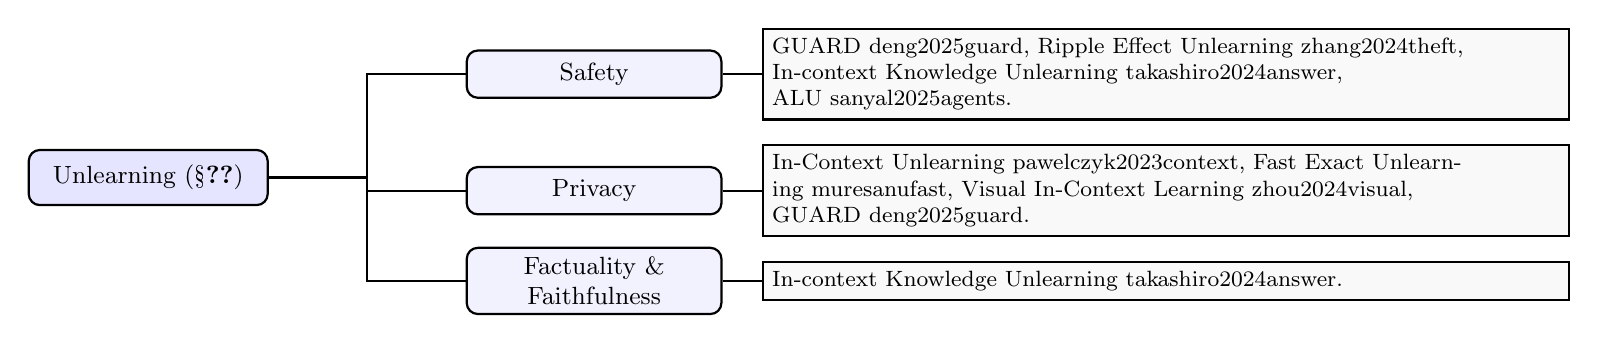
\begin{tikzpicture}
% --- 1. Define leaf nodes (papers, citations added) ---
\node[leaf] (safety_papers) {
GUARD~\citep{deng2025guard}, Ripple Effect Unlearning~\citep{zhang2024theft}, In-context Knowledge Unlearning~\citep{takashiro2024answer}, ALU~\citep{sanyal2025agents}.
};

\node[leaf, below=0.3cm of safety_papers] (privacy_papers) {
In-Context Unlearning~\citep{pawelczyk2023context}, Fast Exact Unlearning~\citep{muresanufast}, 
% Learning to Refuse~\citep{liu2024learning}, 
Visual In-Context Learning~\citep{zhou2024visual}, 
% ECO-Prompts~\citep{liu2024large}, 
GUARD~\citep{deng2025guard}.
};

\node[leaf, below=0.3cm of privacy_papers] (factuality_papers) {
In-context Knowledge Unlearning~\citep{takashiro2024answer}.
};

% --- 2. Define main sub-nodes (Trustworthiness dimensions) ---
% Positioned to the left of corresponding leaf nodes
\node[sub, left=0.5cm of safety_papers] (safety) {Safety};
\node[sub, left=0.5cm of privacy_papers] (privacy) {Privacy};
\node[sub, left=0.5cm of factuality_papers] (factuality) {Factuality \& Faithfulness};

% --- 3. Define root node ---
% Use the calc library to vertically center the root node relative to the sub-nodes
\node[main, left=2.5cm of {$(safety.west)!0.5!(factuality.west)$}] (unlearning) {Unlearning (§\ref{sec:unlearning})};

% --- 4. Draw connection lines ---
% a. Draw a main trunk from the root node to a branching point
\coordinate (fork) at ($(unlearning.east)+(1.25cm,0)$);
\draw[line] (unlearning.east) -- (fork);

% b. Connect from main branching point to each sub-node
\draw[line] (fork) |- (safety.west);
\draw[line] (fork) |- (privacy.west);
\draw[line] (fork) |- (factuality.west);

% c. Connect main sub-nodes directly to leaf nodes
\draw[line] (safety.east) -- (safety_papers.west);
\draw[line] (privacy.east) -- (privacy_papers.west);
\draw[line] (factuality.east) -- (factuality_papers.west);

\end{tikzpicture}%
}
\caption{A taxonomy of Unlearning for enhancing LLM trustworthiness.}
\label{fig:unlearning_taxonomy}
\end{figure}

% LLMs are trained on massive corpora, making it increasingly critical to ensure that they acquire the right knowledge. At the same time, growing legal and ethical concerns have emerged around the presence of unwanted, sensitive, or inappropriate information in these training datasets. These concerns have motivated a surge of interest in machine unlearning.  

% Machine unlearning seeks to selectively remove harmful, private, or copyrighted knowledge from LLMs without retraining them entirely from scratch. Instead, it focuses on erasing the influence of a small subset of undesirable data. In contrast to training-time unlearning—which typically involves gradient ascent or fine-tuning with direct access to the original dataset, and often suffers from instability in controlling weight updates—\textbf{inference-time unlearning} offers a lightweight and dynamic alternative. It enables steering model behavior away from undesirable knowledge while preserving general-purpose capabilities.

\subsubsection{Core Principle.}
% Defines Machine Unlearning as selectively removing information, behaviors, or biases from a pre-trained model, motivated by regulatory needs and safety imperatives.

% Nowadays, Large Language Models are trained on massive text, ensuring the models learned the right knowledge has becoming critical. At the same time, there are growing legal and ethical concerns over LLMs being trained on many unwanted knowledge, which also motivates research into unlearning. 

% Machine unlearning aims to selectively remove harmful, private, or copyrighted knowledge from LLMs without retraining from scratch by leaving out a small subset of unwanted knowledge. In contrast to training-time unlearning, which typically requires gradient ascent or fine-tuning with access to the training set and difficulties of controlling the changes in model weights during this process, inference-time unlearning provides a lightweight, dynamic means of steering model behavior away from undesirable knowledge while preserving general capabilities. 

LLMs are trained on massive corpora, so controlling what knowledge they retain and express has become increasingly important. At the same time, harmful, private, copyrighted, or otherwise undesirable content may be absorbed during training, raising legal, ethical, and safety concerns. These concerns have made unlearning an important problem for trustworthy LLM deployment. At a high level, unlearning aims to prevent targeted knowledge from influencing model behavior. In inference-time settings, this goal is pursued not by rewriting model parameters, but by intervening during generation to suppress, bypass, or reduce the influence of unwanted knowledge and behaviors. Such methods act as runtime control mechanisms. They limit the model's tendency to express targeted content while preserving its broader capabilities. 
% Use some mathematical equations here.

\subsubsection{Mechanisms.}

Inference-time unlearning methods can be grouped into two main families: \emph{gradient-based methods} and \emph{influence-based methods}. Gradient-based methods apply dynamic penalties or control signals during the forward pass to steer generation away from targeted knowledge. Influence-based methods instead estimate and remove the contribution of specific in-context examples at inference time. 

\paragraph{Gradient-Based Methods}
Gradient-based unlearning methods suppress targeted knowledge by applying gradient-inspired penalties during the forward pass. Rather than updating model weights, they modify the model's runtime computation to steer generation away from undesirable outputs.

A representative example is \textbf{GUARD}~\citep{deng2025guard}, which introduces adaptive restriction and detection during generation. By identifying knowledge associated with sensitive concepts and applying penalties in real time, the model is guided away from unsafe continuations while maintaining fluency. Related work also suggests that inference-time forgetting can emerge through runtime control signals that redirect generation toward refusal rather than factual recall~\citep{zhang2024theft}. Overall, these methods make unlearning flexible and reversible at deployment time, but they also highlight a central limitation: the targeted knowledge is often suppressed in output rather than fully erased from the model.


% \paragraph{Gradient-Based Methods}
% % Modifying weights in the opposite direction of the learning gradient (gradient ascent).
% Gradient-based unlearning methods operate by modifying model behavior through gradient signals during inference rather than through permanent weight updates. Instead of training-time fine-tuning, these approaches dynamically adjust activations or steer logits to suppress undesired knowledge. 

% A representative example is GUARD~\citep{deng2025guard}, which introduces adaptive restriction and detection during generation. By identifying knowledge associated with sensitive concepts and applying gradient-inspired penalties in real time, the model is guided to avoid unsafe continuations while maintaining fluency. Similarly, Ripple Effect Unlearning~\citep{zhang2024theft} demonstrates how removing dangerous capabilities (e.g., bomb-making instructions) can propagate across related domains, underscoring both the potential and risks of inference-time gradient steering. Another notable case is In-context knowledge unlearning~\citep{takashiro2024answer}, which employs unlearning tokens to trigger context-dependent forgetting. The model “pretends to forget” by retaining internal activations up to late layers but outputting a refusal token at generation time, illustrating that forgetting is realized as a decision boundary shift rather than true erasure. Together, these works highlight gradient-based unlearning as an inference-time control mechanism: flexible, reversible, and well-suited to safety-critical interventions, though limited by the difficulty of verifying whether knowledge is genuinely erased or merely suppressed. 

% \paragraph{Parameter-Based Methods}
% % Identifying and nullifying parameters storing target information, overlapping with Model Editing.

% Parameter-based methods differ from gradient-based methods in that they do not rely on real-time gradient signals or optimization dynamics. Instead, those methods intervene directly on the model’s internal representations, such as embeddings, neurons, or attention weights, to block the recall of specific knowledge. While gradient-based unlearning operates by steering the model’s computational trajectory during inference, parameter-based methods achieve forgetting by \emph{structural disruption} of how information is encoded. This often yields more stable suppression but with less flexibility compared to gradient-based steering. 

% For example, \textbf{ECO-Prompts}~\citep{liu2024large} corrupt embedding vectors corresponding to unlearning targets, ensuring that when such concepts are queried, the corrupted representations block accurate recall. This lightweight mechanism avoids costly fine-tuning and achieves selective forgetting while preserving unrelated knowledge. Complementary to this, \textbf{Learning to Refuse}~\citep{liu2024learning} adopts a parameter-efficient adaptation strategy, where models are guided to output refusals when sensitive queries are detected. These works illustrate the growing role of parameter-based inference-time unlearning: efficient, composable with other defenses, but often coarse in its selectivity, raising concerns about unintended collateral forgetting. 



% Approximating and subtracting the influence of the "forget" data on final model parameters.
% Influence-based methods differ fundamentally from both gradient-based and parameter-based approaches. 
\paragraph{Influence-Based Methods}

Influence-based methods treat forgetting as the removal or reduction of specific contextual influence at inference time. Rather than steering the model globally, they estimate how particular training or in-context examples contribute to a prediction and then cancel, exclude, or replace that effect during generation. In this sense, they frame unlearning as a counterfactual reasoning problem rather than direct intervention on the forward trajectory.

For example,~\citet{pawelczyk2023context} introduce In-Context Unlearning, where LLMs are taught to disregard selected in-context examples by relabeling or suppressing their contribution, thereby simulating forgetting within the prompt. Building on this idea,~\citet{muresanufast} propose Fast Exact Unlearning, which efficiently removes the influence of in-context training examples from model predictions without weight updates. Although originally motivated by privacy compliance, these methods show how influence estimation can support inference-time unlearning guarantees. This perspective also extends to multimodal settings.~\citet{zhou2024visual} study unlearning in large vision-language models through visual in-context learning and show that selectively excluding visual exemplars at inference time can reduce leakage of sensitive information. Together, these works show that influence-based unlearning is a clean and flexible inference-time mechanism across both text and multimodal generation.

% Unlike gradient-based methods and parameter-based methods, which actively steer the model’s forward computation and modify weights, influence-based approaches work at the level of \emph{attribution}. They approximate and subtract the contribution of specific training or in-context examples to the model’s predictions, effectively simulating what the model would output if those examples had never been present. In this way, they frame unlearning as a counterfactual reasoning problem rather than a direct manipulation of activations or parameters. 

% For instance,~\citet{pawelczyk2023context} introduce \textbf{In-Context Unlearning}, where LLMs are taught to disregard certain in-context examples by re-labeling or suppressing their contribution, thereby simulating forgetting within the prompt. Building on this idea,~\citet{muresanufast} propose \textbf{Fast Exact Unlearning}, which provides efficient algorithms to remove the influence of in-context training examples from LLM predictions without requiring weight updates. While developed primarily for privacy compliance, these methods exemplify how influence estimation can be harnessed to provide test-time unlearning guarantees. Interestingly, work in multimodal settings also extends this perspective. For instance,~\citet{zhou2024visual} investigate unlearning in large vision-language models through visual in-context learning, showing that selectively excluding visual exemplars at inference time can mitigate leakage of sensitive information. Such studies demonstrate that influence-based unlearning is not confined to text, but generalizes to cross-modal reasoning. 

% This typology reveals complementary strengths: gradient-based methods excel in dynamic, safety-critical scenarios; parameter-based approaches provide lightweight suppression via embedding corruption; and influence-based methods approximate counterfactual removal for privacy and compliance. Together, they outline a diverse design space for inference-time unlearning, though verifying true erasure versus behavioral suppression remains an open challenge.

\subsubsection{Applications.}
Although inference-time unlearning methods differ in mechanism, they share a common goal of reducing the influence of harmful, private, or outdated knowledge during generation. Below, we highlight their applications to privacy, safety, and factuality/faithfulness.

\paragraph{Safety}
% Removing dangerous knowledge or toxic language patterns acquired during training.
A key application of unlearning is the suppression of dangerous or toxic capabilities. Because LLMs are trained on large web corpora, they may retain knowledge of illegal activities or unsafe behaviors that can be elicited at deployment time. Gradient-based methods such as GUARD~\citep{deng2025guard} address this problem by applying adaptive restriction and detection during generation, steering the model away from unsafe continuations without retraining. In-context knowledge unlearning~\citep{takashiro2024answer} uses unlearning tokens to trigger selective refusal in context, enabling dynamic suppression of unsafe or irrelevant knowledge. Ripple Effect Unlearning~\citep{zhang2024theft} further shows that suppressing harmful capabilities, such as bomb-making instructions, can reduce jailbreak success but may also propagate to related benign domains. Multi-agent inference frameworks such as ALU~\citep{sanyal2025agents} extend this line by formulating safety control through coordinated unlearning-oriented reasoning under diverse jailbreak settings. 

% Another critical application of unlearning lies in excising dangerous or toxic capabilities. LLMs trained on large web corpora can internalize knowledge of illegal activities or unsafe behaviors, which can pose significant risks during usage without regulations. Gradient-inspired methods such as \emph{GUARD}~\citep{deng2025guard} apply adaptive restriction and detection during generation, steering the model away from unsafe continuations without retraining. \emph{In-context knowledge unlearning}~\citep{takashiro2024answer} introduces unlearning tokens that trigger selective refusal of unsafe or irrelevant knowledge in specific contexts, enabling dynamic, context-aware forgetting. \emph{Ripple Effect Unlearning}~\citep{zhang2024theft} demonstrates that removing harmful capabilities, such as bomb-making instructions, reduces jailbreak success but also reveals unintended propagation effects to benign knowledge domains. In parallel, multi-agent inference pipelines like \emph{ALU}~\citep{sanyal2025agents} evaluate unlearning against a wide range of jailbreak strategies, reinforcing its role in adversarial safety. Together, these works demonstrate unlearning’s promise in mitigating safety risks, while underscoring the importance of managing collateral effects and ensuring consistent refusal across adversarial settings. 

\paragraph{Privacy}
% Removing PII and other sensitive data to comply with privacy regulations and user requests.
Privacy is one of the clearest motivations for unlearning, especially under regulations such as the right to be forgotten~\citep{voigt2017eu, bonta2022california}. Because LLMs can memorize sensitive data and disclose it during interaction, inference-time unlearning provides a lightweight way to reduce such leakage without retraining. In-Context Unlearning~\citep{pawelczyk2023context} suppresses the influence of forgotten examples within the prompt, while Fast Exact Unlearning~\citep{muresanufast} removes the effect of sensitive in-context examples at inference time without changing model parameters. In multimodal settings, Visual In-Context Learning~\citep{zhou2024visual} further shows that excluding visual exemplars at inference time can reduce leakage in large vision-language models. 

% Unlearning is most directly motivated by privacy regulation and the ``right to be forgotten''~\citep{voigt2017eu, bonta2022california}. LLMs are known to memorize sensitive data and may inadvertently disclose it during interactions. Inference-time unlearning provides a lightweight avenue to comply with data deletion requests and protect personally identifiable information (PII) without retraining. Approaches such as \emph{In-Context Unlearning}~\citep{pawelczyk2023context} suppress the contribution of forgotten examples by relabeling or discounting their effect within the prompt, motivated explicitly by GDPR compliance. Building on this, \emph{Fast Exact Unlearning}~\citep{muresanufast} formalizes an efficient algorithm to remove the influence of sensitive in-context examples at inference time, achieving exact compliance without modifying parameters. Parameter-oriented techniques such as \emph{Learning to Refuse}~\citep{liu2024learning} target privacy by attaching a lightweight refusal adapter that maps sensitive queries to refusal tokens, overriding the model’s memorized responses without retraining. Beyond this, \emph{Visual In-Context Learning}~\citep{zhou2024visual} highlights unlearning as essential for secure deployment of large vision-language models in privacy-critical settings. Finally, generation-time defenses such as \emph{GUARD}~\citep{deng2025guard} and \emph{ECO-Prompts}~\citep{liu2024large} define threat models that explicitly include entity leakage and evaluate unlearning methods on datasets containing PII. Collectively, these works highlight unlearning as a crucial defense for privacy protection, though verifying that sensitive knowledge is fully removed rather than suppressed remains an open challenge. 
 
\paragraph{Factuality and Faithfulness}
% 
Inference-time unlearning also relates to factuality and faithfulness, especially when models rely on outdated, incorrect, or untrusted knowledge during generation. Instead of recalling such content, unlearning can redirect the model toward abstention or explicit forgetting. In-context knowledge unlearning~\citep{takashiro2024answer} provides a direct example, showing that unlearning tokens can suppress forgotten content and induce explicit ``forgotten'' responses rather than unsupported answers. This suggests that inference-time unlearning can improve factual reliability by preventing the model from expressing knowledge that should no longer be trusted. At the same time, this connection remains underexplored, and it is still unclear when runtime suppression should be viewed as genuine forgetting rather than controlled abstention. Recent diagnostic frameworks argue that single-value unlearning metrics obscure exactly this distinction, and propose cognitive-diagnosis-style evaluations that jointly probe retention, removal, and transfer effects across difficulty levels~\citep{lang2025beyond}.

% \subsubsection{Discussion: The Verification Problem and Conceptual Unlearning}
% % Strengths: Provides a targeted and efficient solution for data removal and harm mitigation.
% % Limitations: The fundamental difficulty of verifying that information is truly forgotten, the utility-forgetting trade-off, and the challenge of unlearning abstract concepts versus specific data points.


% \paragraph{Strength}

% % A key strength of inference-time unlearning lies in its ability to provide \textbf{targeted control over model generation}. Rather than permanently altering parameters, these methods allow model practitioners to precisely steer outputs away from sensitive or harmful knowledge while preserving the model’s broader utility. This controllability makes them particularly suitable for dynamic and safety-critical settings where reversibility and fine-grained adjustment are essential. At the same time, inference-time unlearning is inherently \textbf{lightweight and efficient}: it avoids the prohibitive costs of retraining or weight-level editing, instead intervening directly during inference through activation steering, parameter masking, or influence subtraction. Together, these properties make inference-time approaches not only more practical for real-world deployment, but also more adaptable to evolving regulatory and ethical demands where responsiveness is as important as robustness.

% A key strength of inference-time unlearning is its targeted control over model generation. Rather than changing model parameters, these methods steer outputs away from sensitive or harmful knowledge while preserving broader utility. This makes them especially useful in dynamic or safety-critical settings where reversibility and fine-grained adjustment matter. They are also lightweight and efficient. Instead of relying on retraining or offline model modification, they intervene during generation through runtime penalties, control signals, or influence subtraction. These properties make inference-time unlearning practical for deployment and adaptable to evolving safety, privacy, and regulatory demands.


% \paragraph{Limitations}

% % Despite these strengths, inference-time unlearning still faces several critical limitations. One major challenge is the \textbf{robustness of unlearning}. Prior work shows that many algorithms tend to obscure unlearned knowledge rather than erasing it entirely, leaving models vulnerable to recovery under adversarial prompting or indirect probing attacks~\citep{lucki2024adversarial, dou2025avoiding}. This casts doubt on whether inference-time suppression can provide the strong deletion guarantees demanded in privacy and safety-sensitive applications. Another limitation is the \textbf{trade-off between utility and unlearning efficacy}. As recent studies demonstrate~\citep{liu2024breaking, liu2024towards}, achieving stronger unlearning often comes at the cost of reduced fluency, accuracy, or reasoning ability, echoing the “alignment tax” observed in RLHF settings~\citep{lin2023mitigating}. This tension highlights an open research problem: designing inference-time algorithms that maintain high utility while reliably mitigating harmful or sensitive knowledge. Addressing both robustness and the utility–efficacy trade-off will be essential for advancing inference-time unlearning from a promising intervention into a dependable component of trustworthy LLM deployment.

% Despite these strengths, inference-time unlearning still faces important limitations. One major challenge is verification. Many methods appear to suppress unlearned knowledge rather than remove its influence entirely, which leaves models vulnerable to recovery under adversarial prompting or indirect probing~\citep{lucki2024adversarial, dou2025avoiding}. This makes it difficult to determine whether a method achieves genuine forgetting or only output-level suppression. Another challenge is the trade-off between utility and unlearning strength. Stronger suppression can reduce harmful or sensitive outputs, but it may also hurt fluency, accuracy, or reasoning ability~\citep{liu2024breaking, liu2024towards, lin2023mitigating}. Addressing both verification and this utility trade-off will be important for making inference-time unlearning a dependable part of trustworthy LLM deployment.

% \section{Pruning}
% \label{sec:pruning}

% \subsection{Core Principle: A Paradigm Shift from Efficiency to Trustworthiness}
% % Defines Pruning as the selective removal of model components (weights, neurons, heads), reframing it from a compression technique to a coarse-grained tool for enhancing trust.
% Model pruning has historically been framed as a technique for computational efficiency to reduce inference cost, shrink memory footprint, and accelerate deployment. Yet as large-scale models are increasingly embedded into deployed real systems, the primary motivation for pruning has shifted. Instead of simply optimizing speed and size, pruning is now leveraged as a means of enhancing trustworthiness across dimensions such as safety, fairness, privacy, factuality, and faithfulness.
% In this new paradigm, pruning is not just about discarding redundant parameters. It becomes a form of structural governance over model behavior. By carefully identifying and removing connections or subnetworks associated with bias amplification, unsafe generations, or privacy-leaking pathways, pruning can reshape the representational space of models in ways that support responsible AI deployment.
% Mechanisms such as fairness-aware sparsification, safety-constrained pruning, and privacy-preserving structural reduction highlight this transformation. Rather than treating trustworthiness as an external add-on, pruning integrates it directly into the model’s internal architecture. This reorientation establishes pruning as not only a tool for efficiency, but as a principle for building leaner, safer, and more equitable models.

% \subsection{Applications in Trustworthiness Dimensions}

% Recent studies increasingly show that looking only at perplexity or utility hides important safety shifts. A multi-dimensional audit found that compression affects degeneration harm (toxicity or stereotypes), representational harms, and dialect bias differently, and that pruning tends to degrade safety faster than quantization as sparsity rises—making safety evaluation integral to pruning pipelines, not an afterthought. Therefore, treating safety as a first-class constraint in pruning is very important by attributing safety-critical neurons before sparsification is very important. Current research prefers training-free repair (HSR, NLSR, SafePTR) when deployment constraints preclude retraining, and includes safety metrics in pruning method design, not just perplexity or task accuracy.

% \subsubsection{Safety}
% % Used to remove subnetworks hypothesized to be responsible for unsafe behaviors, potentially increasing the robustness of alignment.


% \textbf{Safety is Brittle in Traditional Pruning} Study~\citep{wei2024assessing} identifies that, removing ~3\% of parameters (or ~2.5\% ranks) in safety-critical regions sharply harms refusal behavior without large utility loss, which evidence that aligned safety is structurally sparse and thus fragile to pruning. Research~\citep{zhang2025activation} reveals that activation approximations for model efficiency can undercut safety across methods and models. In light of this, the authors propose approximation-aware re-alignment to patch these safety losses.

% \textbf{Repair safety by Pruning models.}
% Hierarchical Safety Realignment (HSR) for LVLMs~\citep{li-etal-2025-hierarchical} attributes safety contribution at the head level, then selectively restores only a small set of neurons in those critical heads to recover safety after pruning, which is lightweight and training-free. Safety-specific neurons (SN-Tune)~\citep{zhao2025understanding} claims that safety circuitry is sparse, language-specific, and concentrated in early self-attention layers; tuning just these neurons restores safety with minimal utility impact—supporting “localizable” safety factors that pruning can inadvertently remove. Neuron-Level Safety Realignment (NLSR)~\citep{yi2025nlsr} proposes that when harmful fine-tuning compromises alignment, identify safety-critical neurons by similarity to a reference aligned model and transplant only those neurons—training-free restoration with preserved task accuracy. In SafePTR~\citep{chen2025safeptr}, the authors mention token-level pruning at vulnerable layers followed by feature restoration in later layers improves jailbreak resistance across multiple MLLMs while retaining utility.~\citep{sawtell2024lightweight} uses a pruned LM as a frozen feature extractor and trains a penalized logistic head at the best intermediate layer to detect content-safety violations and prompt injection—smaller, faster safety filters.~\citep{hasan2024pruning} claims that moderate attention-focused sparsity (~20\% in attention) can increase jailbreak resistance in already-aligned models without fine-tuning, though gains correlate with the model’s initial safety level and are not universal. Attention Pruning~\citep{dasu2025attention} learns a surrogate mapping from head on/off states to fairness/utility, then searches the Pareto front to prune bias-amplifying heads—reporting up to ~40\% gender-bias reduction.



% \subsubsection{Fairness}
% % Used to remove components, such as specific attention heads, that have been identified as major contributors to societal bias.
% Structured fairness pruning helps the LLM to keep general performance while improving model fairness. Fairness-Aware Structured Pruning (FASP)~\citep{zayed2024fairness} identifies attention heads that harm fairness but contribute little to language modeling, pruning them to reduce gender bias (8–40\% depending on model) with only slight utility drops; code and figures detail the head-selection logic.

% There are also some pruning for fairness research finds that pruning needs to pay attention to generalization, data, and attention mechanism. A systematic study on racial bias~\citep{ma2025breaking} finds neuron-level pruning generally outperforms head-level pruning for fairness, but fairness gains deteriorate when moving across contexts (e.g., financial decisions to commercial transactions), underscoring context-specific bias mechanisms and limited one-shot generalizability. Study claims that~\citep{bandari-etal-2024-c4} the dataset used to score importance during pruning strongly shapes outcomes: C4 is not universally optimal; arithmetic data can sometimes calibrate better; and pruning with a downstream dataset doesn’t necessarily help that very downstream task—implying fairness evals should be co-designed with calibration data selection. Study~\citep{zayed2024fairness} first investigates how attention heads impact fairness and performance in pre-trained transformer-based language models. The authors then propose a novel method to prune the attention heads that negatively impact fairness while retaining the heads critical for performance. This approach is practical in terms of time and resources, as it does not require fine-tuning the final pruned fairer model. 


% \subsubsection{Privacy, Factuality and Faithfulness}
% \textbf{Privacy} Dissecting LMs~\citep{pochinkov2024dissecting} proposes removing neurons specialized for undesired behaviors while preserving overall performance by data-efficient unlearning via pruning. Follow-ups like LLM-Eraser formalize a two-stage localize then unlearn process to erase harmful or sensitive knowledge more precisely. For MLLMs, modality-aware neuron selection~\citep{liu-etal-2025-modality} selective pruning balances forgetting targeted private data across modalities while retaining core capability. In federated pruning for privacy-sensitive domains, FedPrLLM~\citep{guo2025exploring} lets clients compute and share only pruning masks (no raw data), enabling a server to aggregate a globally pruned model, which reduces reliance on public calibration data and keeps local data private. 

% \textbf{Factuality} A large study~\citep{chrysostomou2024investigating} on abstractive summarization (5 LLMs, 2 pruning methods, 5 datasets) finds pruned models hallucinate less and rely more on source content (higher lexical overlap), suggesting pruning can filter spurious pathways and nudge models toward evidence-based generation such as summarization. Generalization to other tasks still needs testing.

% \textbf{Faithfulness}
% Faithfulness framework~\citep{lanham2023measuring} show that CoT-style explanations can be unfaithful to internal reasoning; evaluations intervene on the CoT or model to probe causal dependence. While there isn’t yet a pruning-specific faithfulness benchmark, combining (i) the hallucination reduction result above and (ii) safety-neuron localization findings suggests a path: prune shortcut-driven or “ungrounded” units, then validate with faithfulness tests (e.g., CoT intervention/unlearning-based diagnostics). 

% \subsection{Discussion: The Blunt Instrument Dilemma}
% % Strengths: Offers a permanent, parameter-reducing intervention that can completely remove certain functionalities.
% % Limitations: Pruning is a coarse-grained "blunt instrument"; components are often polysemantic, making it difficult to remove bad behaviors without degrading good ones, and identification of what to prune is a major challenge.

\subsection{Pruning}

\begin{figure}[htbp]
\centering
% Width uses \textwidth; height auto-scales with !
\resizebox{\textwidth}{!}{%
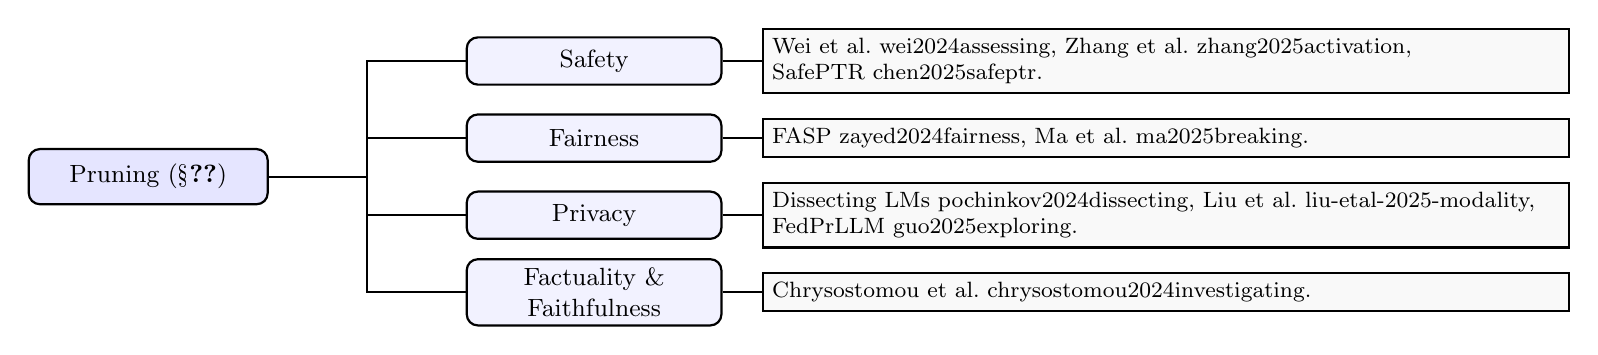
\begin{tikzpicture}
% % --- 1. Define leaf nodes (papers, citations added) ---
% \node[leaf] (safety_papers) {
% Wei et al.~\citep{wei2024assessing}, Zhang et al.~\citep{zhang2025activation}, HSR~\citep{li-etal-2025-hierarchical}, SN-Tune~\citep{zhao2025understanding}, NLSR~\citep{yi2025nlsr}, SafePTR~\citep{chen2025safeptr}, Sawtell et al.~\citep{sawtell2024lightweight}, Hasan et al.~\citep{hasan2024pruning}.
% };
% \node[leaf, below=0.3cm of safety_papers] (fairness_papers) {
% FASP~\citep{zayed2024fairness}, Ma et al.~\citep{ma2025breaking}, Bandari et al.~\citep{bandari-etal-2024-c4}, Attention-State Pruning~\citep{dasu2025attention}.
% };
% \node[leaf, below=0.3cm of fairness_papers] (privacy_papers) {
% Dissecting LMs~\citep{pochinkov2024dissecting}, Liu et al.~\citep{liu-etal-2025-modality}, FedPrLLM~\citep{guo2025exploring}.
% };
% \node[leaf, below=0.3cm of privacy_papers] (factuality_papers) {
% Chrysostomou et al.~\citep{chrysostomou2024investigating}, Lanham et al.~\citep{lanham2023measuring}.
% };

% --- 1. Define leaf nodes (papers, citations added) ---
\node[leaf] (safety_papers) {
Wei et al.~\citep{wei2024assessing}, Zhang et al.~\citep{zhang2025activation}, SafePTR~\citep{chen2025safeptr}.
};
\node[leaf, below=0.3cm of safety_papers] (fairness_papers) {
FASP~\citep{zayed2024fairness}, Ma et al.~\citep{ma2025breaking}.
};
\node[leaf, below=0.3cm of fairness_papers] (privacy_papers) {
Dissecting LMs~\citep{pochinkov2024dissecting}, Liu et al.~\citep{liu-etal-2025-modality}, FedPrLLM~\citep{guo2025exploring}.
};
\node[leaf, below=0.3cm of privacy_papers] (factuality_papers) {
Chrysostomou et al.~\citep{chrysostomou2024investigating}.
};

% --- 2. Define main sub-nodes (Trustworthiness dimensions) ---
% Positioned to the left of corresponding leaf nodes
\node[sub, left=0.5cm of safety_papers] (safety) {Safety};
\node[sub, left=0.5cm of fairness_papers] (fairness) {Fairness};
\node[sub, left=0.5cm of privacy_papers] (privacy) {Privacy};
\node[sub, left=0.5cm of factuality_papers] (factuality) {Factuality \& Faithfulness};
% --- 3. Define root node ---
% Use the calc library to vertically center the root node relative to the sub-nodes
\node[main, left=2.5cm of {$(safety.west)!0.5!(factuality.west)$}] (pruning) {Pruning (§\ref{sec:pruning-core})};
% --- 4. Draw connection lines ---
% a. Draw a main trunk from the root node to a branching point
\coordinate (fork) at ($(pruning.east)+(1.25cm,0)$);
\draw[line] (pruning.east) -- (fork);
% b. Connect from main branching point to each sub-node
\draw[line] (fork) |- (safety.west);
\draw[line] (fork) |- (fairness.west);
\draw[line] (fork) |- (privacy.west);
\draw[line] (fork) |- (factuality.west);
% c. Connect main sub-nodes directly to leaf nodes
\draw[line] (safety.east) -- (safety_papers.west);
\draw[line] (fairness.east) -- (fairness_papers.west);
\draw[line] (privacy.east) -- (privacy_papers.west);
\draw[line] (factuality.east) -- (factuality_papers.west);
\end{tikzpicture}%
}
\caption{A taxonomy of Pruning for enhancing LLM trustworthiness.}
\label{fig:pruning_taxonomy}
\end{figure}

\subsubsection{Core Principle.}
\label{sec:pruning-core}

% Pruning has traditionally been justified as an efficiency tool—reducing inference cost, memory footprint, and latency. As foundation models move from research prototypes to safety- and regulation–constrained deployments, this framing is incomplete. The motivation is shifting from \emph{how fast and small} to \emph{how safe, fair, private, and faithful}. 

% In this view, pruning is not merely the removal of redundant weights; it is \textbf{structural governance} over behavior. By identifying and excising connections or subnetworks implicated in bias amplification, unsafe generations, or privacy leakage, pruning reshapes representational pathways to support responsible deployment. Mechanisms such as fairness-aware sparsification, safety-constrained pruning, and privacy-preserving structural reduction embed trust objectives inside the architecture itself rather than treating them as after-the-fact add-ons. This reorientation positions pruning as a principle for building leaner, safer, and more equitable models—not only a vehicle for speedups.

Pruning has traditionally been studied as a tool for improving efficiency by reducing inference cost, memory footprint, and latency. As foundation models move into safety- and regulation-sensitive settings, this framing is no longer sufficient. The key question is no longer only how to make models smaller or faster, but also how to make them safer, fairer, more privacy-preserving, and more reliable.

From this perspective, pruning becomes a form of structural control over model behavior rather than a purely efficiency-driven reduction technique. By selectively suppressing weights, neurons, heads, or subnetworks associated with bias amplification, unsafe generation, or privacy leakage, pruning can reshape the pathways through which the model produces outputs. Methods such as fairness-aware sparsification, safety-constrained pruning, and privacy-oriented structural reduction reflect this shift by embedding trust-related objectives into the model's active computation rather than treating them only as post hoc corrections. Under this view, pruning serves not only to improve efficiency, but also to support leaner and more trustworthy deployment.

\subsubsection{Applications.}
\label{sec:pruning-dimensions}

% Empirical evidence shows that looking only at perplexity/utility can mask significant safety shifts. Multi-axis audits report that compression differentially affects degeneration harms (toxicity/stereotypes), representational harms, and dialect bias, and that sparsification often harms safety faster than quantization as sparsity increases. Consequently, safety must be treated as a first-class constraint in pruning: attribute safety-critical units \emph{before} sparsification and include safety metrics \emph{during} method design, not as an afterthought. When retraining is infeasible, training-free repair methods (e.g., HSR, NLSR, SafePTR) are increasingly preferred, as they restore safety with minimal compute and drift.

Empirical evidence shows that utility metrics alone can miss important trustworthiness shifts after pruning. Compression may preserve perplexity while still degrading refusal behavior, toxicity control, or other safety properties. This means safety should be treated as a first-class constraint in pruning rather than checked only after compression.


\paragraph{Safety}
\label{sec:pruning-safety}

% \paragraph{Brittleness under naive pruning.}
%~\citet{wei2024assessing} show that removing only $\sim$3\% of parameters (or $\sim$2.5\% ranks) in safety-critical regions sharply degrades refusal behavior despite small utility loss, indicating aligned safety is structurally sparse—and fragile—to pruning.~\citet{zhang2025activation} further find that activation approximations for efficiency can undercut safety across models and methods, motivating approximation-aware realignment to patch these losses.

% \paragraph{Safety repair via structure-aware pruning and restoration.}
% For LVLMs, \textbf{HSR}~\citep{li-etal-2025-hierarchical} attributes safety at the \emph{head} level and selectively restores a small neuron subset in critical heads post-pruning—lightweight and training-free. \textbf{SN-Tune}~\citep{zhao2025understanding} localizes safety circuitry to sparse, language-specific neurons concentrated in early self-attention; tuning only these units restores refusals with minimal utility impact, explaining why indiscriminate pruning can remove them. \textbf{NLSR}~\citep{yi2025nlsr} detects safety-critical neurons by similarity to a reference aligned model and transplants only those neurons, preserving accuracy while re-aligning refusals. \textbf{SafePTR}~\citep{chen2025safeptr} combines token-level pruning at vulnerable layers with feature restoration downstream, improving jailbreak resistance across MLLMs. Complementary approaches include using a pruned LM as a frozen feature extractor with a penalized logistic head for content-safety and prompt-injection detection~\citep{sawtell2024lightweight}, and observations that moderate attention-focused sparsity ($\sim$20\%) can harden already-aligned models, albeit non-universally~\citep{hasan2024pruning}. Finally, \textbf{attention-state pruning} learns a surrogate from head on/off patterns to fairness–utility trade-offs and searches the Pareto front to prune bias-amplifying heads~\citep{dasu2025attention}.

Naive pruning can weaken safety even when utility loss is small.~\citet{wei2024assessing} show that removing only $\sim$3\% of parameters, or $\sim$2.5\% of low-rank components, in safety-critical regions can sharply degrade refusal behavior, suggesting that aligned safety depends on structurally sparse components.~\citet{zhang2025activation} further show that efficiency-oriented activation approximation can also introduce safety vulnerabilities, reinforcing the need to account for safety during compression rather than after it. Recent work therefore explores more targeted pruning strategies. In multimodal LLMs, SafePTR~\citep{chen2025safeptr} selectively prunes harmful tokens at vulnerable layers and restores benign features at later layers, improving jailbreak resistance while preserving utility. Overall, these results suggest that pruning can support safety only when the intervention is explicitly trust-aware. Otherwise, compression may remove precisely the components that sustain aligned behavior.


\paragraph{Fairness}
\label{sec:pruning-fairness}

Fairness-oriented pruning is less clearly aligned with inference-time trustworthiness than safety-oriented runtime pruning. Existing work mainly studies post-processing structural interventions, such as pruning attention heads associated with bias or comparing head- and neuron-level pruning for bias mitigation~\citep{zayed2024fairness, ma2025breaking}. These results suggest that selective structural suppression can reduce bias, but they are better viewed as adjacent pruning-based debiasing methods than as clean inference-time interventions. As a result, fairness remains relatively underexplored for pruning under the stricter inference-time setting considered here.

% \paragraph{Structured pruning.}
% \textbf{FASP}~\citep{zayed2024fairness} identifies attention heads that harm fairness yet contribute little to language modeling, pruning them to reduce gender bias (8–40\% depending on model) with minor utility drops; the head-selection logic and code are released.

% \paragraph{Generalization, data choice, and mechanism.}
% A racial-bias study finds neuron-level pruning generally outperforms head-level pruning for fairness, but gains deteriorate when moving across domains (e.g., financial $\rightarrow$ commercial), underscoring context-specific bias mechanisms and limited one-shot generalization~\citep{ma2025breaking}. Data used to score importance strongly shapes outcomes: C4 is not universally optimal; arithmetic data can sometimes calibrate better; and pruning with a downstream dataset does not necessarily help that very task~\citep{bandari-etal-2024-c4}. Together with~\citet{zayed2024fairness}, these results argue for co-design of fairness evaluation with calibration data selection and for mechanism-aware (head vs.\ neuron) sparsification.

\paragraph{Privacy}
Pruning has also been explored for privacy protection, though much of this work is closer to deployment-oriented structural intervention than to strict runtime control during generation. Existing methods identify and remove neurons or subnetworks associated with memorized sensitive content, aiming to suppress privacy leakage while preserving general utility. Examples include data-efficient neuron pruning in language models, modality-aware pruning in MLLMs, and federated pruning schemes that exchange pruning masks rather than raw data~\citep{pochinkov2024dissecting, liu-etal-2025-modality, guo2025exploring}. These results suggest that pruning can support privacy-preserving deployment, but most current methods rely on structural modification before deployment rather than conditional pruning at inference time.

\paragraph{Factuality and Faithfulness}
Pruning has also shown some potential for improving factual reliability, although evidence remains limited. One large summarization study reports that pruned models hallucinate less and rely more on source content, suggesting that pruning may suppress spurious generation pathways~\citep{chrysostomou2024investigating}. However, it is still unclear whether this effect transfers beyond summarization or supports stronger notions of faithfulness. At present, factuality and faithfulness remain promising but underexplored directions for pruning in trustworthy model deployment.

% \paragraph{Privacy, Factuality, and Faithfulness}
% \label{sec:pruning-privacy-fact}

% \paragraph{Privacy.}
% \textbf{Dissecting LMs}~\citep{pochinkov2024dissecting} removes neurons specialized for undesired behaviors via data-efficient unlearning through pruning, preserving overall performance. Follow-ups (e.g., LLM-Eraser) formalize \emph{localize\,\textrightarrow\,unlearn} workflows for precise erasure. In MLLMs, \emph{modality-aware} neuron selection prunes to forget private data while retaining core capability~\citep{liu-etal-2025-modality}. In privacy-sensitive federated settings, \textbf{FedPrLLM}~\citep{guo2025exploring} aggregates only pruning masks across clients (no raw data), reducing reliance on public calibration data and preserving local privacy.

% \paragraph{Factuality.}
% A large abstractive-summarization study (5 LLMs, 2 pruning methods, 5 datasets) reports that pruned models hallucinate less and rely more on source content (higher lexical overlap), suggesting pruning can suppress spurious pathways and nudge models toward evidence-based generation~\citep{chrysostomou2024investigating}. Whether this effect transfers beyond summarization remains open.

% \paragraph{Faithfulness.}
% Faithfulness evaluations show CoT explanations can be unfaithful to internal reasoning~\citep{lanham2023measuring}. While pruning-specific faithfulness benchmarks are nascent, two strands point to a practical recipe: (i) pruning reduces shortcut-driven hallucinations in summarization~\citep{chrysostomou2024investigating}; (ii) safety-neuron localization suggests targeted removal of “ungrounded” units. A promising protocol is to prune candidate shortcut circuits, then validate with causal faithfulness tests (e.g., CoT intervention or unlearning-style diagnostics).



% \subsubsection{Discussion}
% \label{sec:pruning-discussion}

% \paragraph{Takeaways.}
% Across dimensions, pruning should (1) attribute trust-critical structure prior to sparsification, (2) optimize for multi-objective trade-offs (utility \emph{and} safety/fairness/privacy), and (3) include post-pruning repair paths that are training-free when deployment 

% \paragraph{Strengths}
% A trust-centric view of pruning offers \textbf{direct, structural control} over model behavior. By acting on interpretable units (layers, heads, neurons), practitioners can align architectural pathways with policy goals (safety, fairness, privacy) rather than relying solely on post hoc filtering. This yields auditable interventions: which units were removed, why, and with what effect can be documented and revisited.
% Second, pruning enables multi-objective co-optimization of efficiency and trust. Many of the safety/fairness–aware methods are training-free or minimally adaptive (e.g., targeted restoration), making them attractive under tight deployment budgets. Pruning is also composable with quantization, KV-cache strategies, or distillation, offering an orthogonal lever in practical pipelines.
% Finally, the paradigm generalizes beyond text. Modality-aware selection in MLLMs and mask aggregation in federated settings demonstrate that structural governance via pruning can support privacy and safety constraints under diverse data and orchestration regimes.

% \paragraph{Limitations}
% The same sparsity that makes safety circuits identifiable can render them fragile: small amounts of indiscriminate sparsification can collapse refusal behavior or fairness gains. Importance scores that drive pruning decisions are noisy and data-dependent; attribution errors produce collateral damage (utility loss, new biases), and gains may not generalize across domains or dialects.
% Pruning alone does not close adversarial gaps. Attackers can route around removed paths; defenses require complementary detection/refusal layers and continual red-teaming. From a systems perspective, unstructured masks often underutilize hardware; structured sparsity or block-level designs are needed to realize speedups on modern accelerators.
% Evaluation remains a bottleneck. Trustworthiness effects are under-measured: multi-turn, long-horizon, and domain-shifted audits are rare; trade-off fronts (utility–safety–fairness–privacy) are seldom reported with confidence intervals. Finally, current methods lack formal guarantees (privacy erasure vs.\ suppression, causal fairness bounds) and can drift after further fine-tuning or continued pretraining unless masks and metrics are versioned and monitored.




% --- Tier 3: System-Level Orchestration ---
\section{System-Level Orchestration}
\label{sec:system_level}
System-level orchestration moves beyond single-model interventions to coordinate multiple LLM agents into collaborative architectures. Rather than controlling one model in isolation, trustworthiness here emerges from structured interaction patterns---debate, cross-verification, role specialization, and iterative self-correction. In the inference-time pipeline (Figure~\ref{fig:taxonomy_pipeline}), the tool-use / agents loop spans context assembly, generation, and output checking, creating feedback cycles that enable collective reliability.

%% ============================================================
%% Revision Notes (2026-03-29, Yuyang):
%% 1. Core Principle: Already concise, kept as-is.
%% 2. Applications: Ensured each domain is one paragraph. Merged
%%    Fairness sub-themes (Cultural Adaptability + Demographic Fairness).
%%    Compressed Privacy into one paragraph. Cleaned up commented-out
%%    old versions of Safety and Factuality.
%% 3. Discussion: Removed from this file. Shortened version moved to
%%    sections/11-challenges_directions.tex with red source marker.
%% ============================================================

\subsection{Multi-Agent Systems}
\label{sec:multi_agent_systems}

\begin{figure}[htbp]
    \centering
    % Width uses \textwidth; height auto-scales with !
    \resizebox{\textwidth}{!}{%
        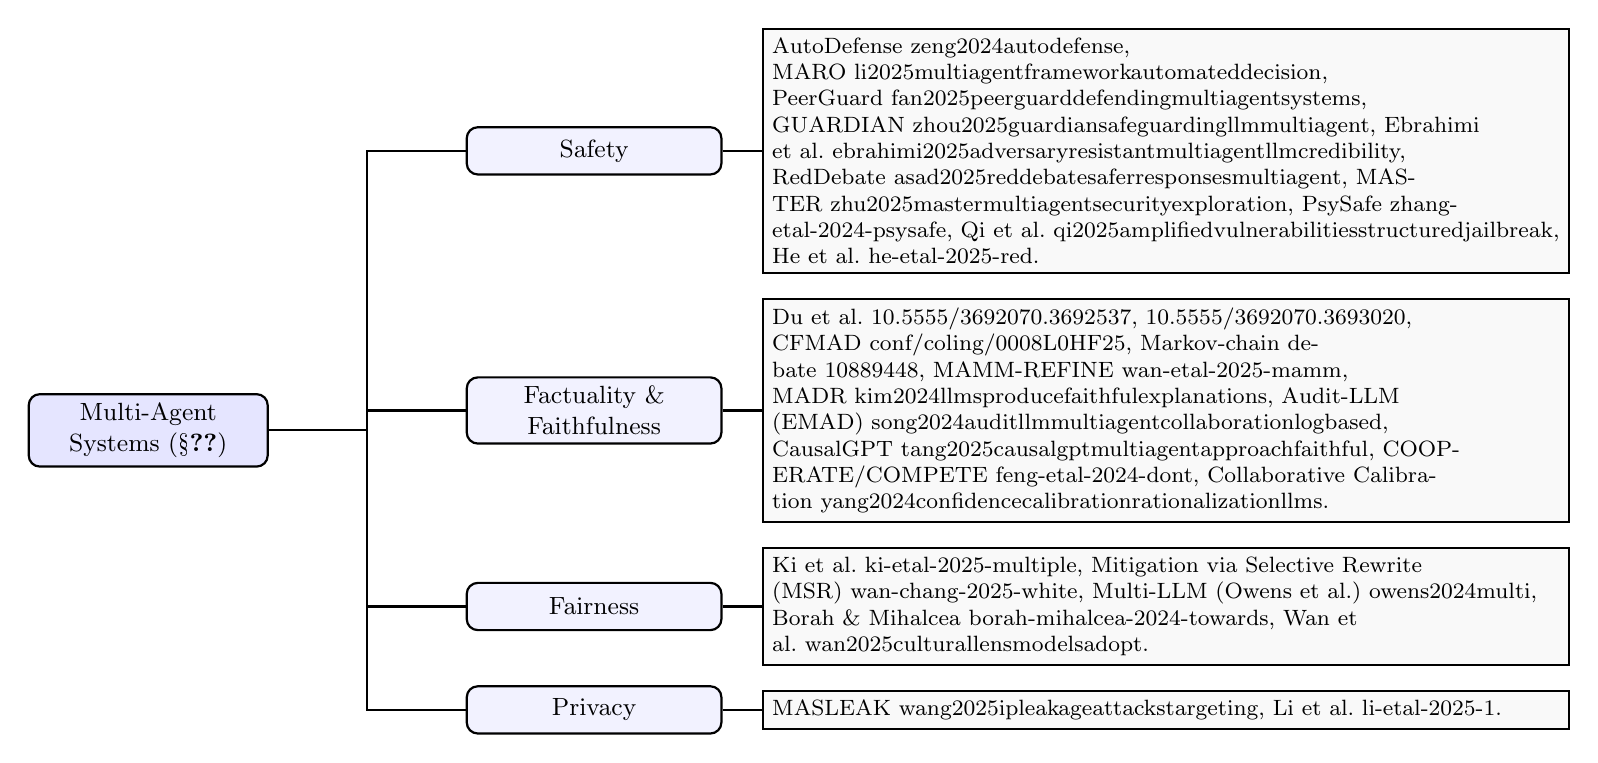
\begin{tikzpicture}

        % --- 1. Define leaf nodes (papers, citations added) ---
        \node[leaf] (safety_papers) {
            AutoDefense~\citep{zeng2024autodefense}, MARO~\citep{li2025multiagentframeworkautomateddecision}, PeerGuard~\citep{fan2025peerguarddefendingmultiagentsystems}, GUARDIAN~\citep{zhou2025guardiansafeguardingllmmultiagent}, Ebrahimi et al.~\citep{ebrahimi2025adversaryresistantmultiagentllmcredibility}, RedDebate~\citep{asad2025reddebatesaferresponsesmultiagent}, MASTER~\citep{zhu2025mastermultiagentsecurityexploration}, PsySafe~\citep{zhang-etal-2024-psysafe}, Qi et al.~\citep{qi2025amplifiedvulnerabilitiesstructuredjailbreak}, He et al.~\citep{he-etal-2025-red}.
        };
        \node[leaf, below=0.3cm of safety_papers] (factuality_papers) {
            Du et al.~\citep{10.5555/3692070.3692537, 10.5555/3692070.3693020}, CFMAD~\citep{conf/coling/0008L0HF25}, Markov-chain debate~\citep{10889448}, MAMM-REFINE~\citep{wan-etal-2025-mamm}, MADR~\citep{kim2024llmsproducefaithfulexplanations}, Audit-LLM (EMAD)~\citep{song2024auditllmmultiagentcollaborationlogbased}, CausalGPT~\citep{tang2025causalgptmultiagentapproachfaithful}, COOPERATE/COMPETE~\citep{feng-etal-2024-dont}, Collaborative Calibration~\citep{yang2024confidencecalibrationrationalizationllms}.
        };
        \node[leaf, below=0.3cm of factuality_papers] (fairness_papers) {
            Ki et al.~\citep{ki-etal-2025-multiple}, Mitigation via Selective Rewrite (MSR)~\citep{wan-chang-2025-white}, Multi-LLM (Owens et al.)~\citep{owens2024multi}, Borah \& Mihalcea~\citep{borah-mihalcea-2024-towards}, Wan et al.~\citep{wan2025culturallensmodelsadopt}.
        };
        \node[leaf, below=0.3cm of fairness_papers] (privacy_papers) {
            MASLEAK~\citep{wang2025ipleakageattackstargeting}, Li et al.~\citep{li-etal-2025-1}.
        };

        % --- 2. Define main sub-nodes (Trustworthiness dimensions) ---
        % Positioned to the left of corresponding leaf nodes
        \node[sub, left=0.5cm of safety_papers] (safety) {Safety};
        \node[sub, left=0.5cm of factuality_papers] (factuality) {Factuality \& Faithfulness};
        \node[sub, left=0.5cm of fairness_papers] (fairness) {Fairness};
        \node[sub, left=0.5cm of privacy_papers] (privacy) {Privacy};

        % --- 3. Define root node ---
        % Use the calc library to vertically center the root node relative to the sub-nodes
        \node[main, left=2.5cm of {$(safety.west)!0.5!(privacy.west)$}] (mas) {Multi-Agent Systems (§\ref{sec:multi_agent_systems})};

        % --- 4. Draw connection lines ---
        % a. Draw a main trunk from the root node to a branching point
        \coordinate (fork) at ($(mas.east) + (1.25cm,0)$);
        \draw[line] (mas.east) -- (fork);

        % b. Connect from main branching point to each sub-node
        \draw[line] (fork) |- (safety.west);
        \draw[line] (fork) |- (factuality.west);
        \draw[line] (fork) |- (fairness.west);
        \draw[line] (fork) |- (privacy.west);

        % c. Connect main sub-nodes directly to leaf nodes
        \draw[line] (safety.east) -- (safety_papers.west);
        \draw[line] (factuality.east) -- (factuality_papers.west);
        \draw[line] (fairness.east) -- (fairness_papers.west);
        \draw[line] (privacy.east) -- (privacy_papers.west);

        \end{tikzpicture}%
    }
    \caption{A taxonomy of Multi-Agent Systems for enhancing LLM trustworthiness.}
    \label{fig:mas_taxonomy}
\end{figure}

Multi-Agent Systems (MAS) represents a fundamental paradigm shift in controlling LLM behavior. Instead of focusing on a single, monolithic model, this approach architects a system of multiple, interacting LLM-based agents. Within this framework, trustworthiness is not a property enforced upon a single model but rather an emergent property of the system's collaborative dynamics. By structuring interactions through mechanisms such as debate, adversarial simulation, and multi-perspective deliberation, MAS can achieve levels of robustness, safety, and factuality that are often unattainable by individual agents.

\subsubsection{Core Principle: From Monolithic Control to Collaborative Systems}

The core principle of multi-agent systems is the decentralization of reasoning and decision-making. A complex problem is decomposed and assigned to specialized agents, each potentially embodying a unique role, persona, or expertise. Trustworthiness is fostered through the design of their interaction protocols, which can include adversarial debate, cooperative problem-solving, peer review, or hierarchical verification. For instance, a ``propose'' agent might generate an initial response, a ``critic'' agent might challenge its assumptions and check for flaws, and a ``synthesize'' agent might integrate the feedback to produce a final, more considered output. This structured interaction creates an intrinsic error-correction and validation mechanism at inference time. The system's reliability, therefore, depends less on the perfection of any single agent and more on the robustness of the collaborative architecture itself.


\begin{figure*}[htbp]
  \centering
  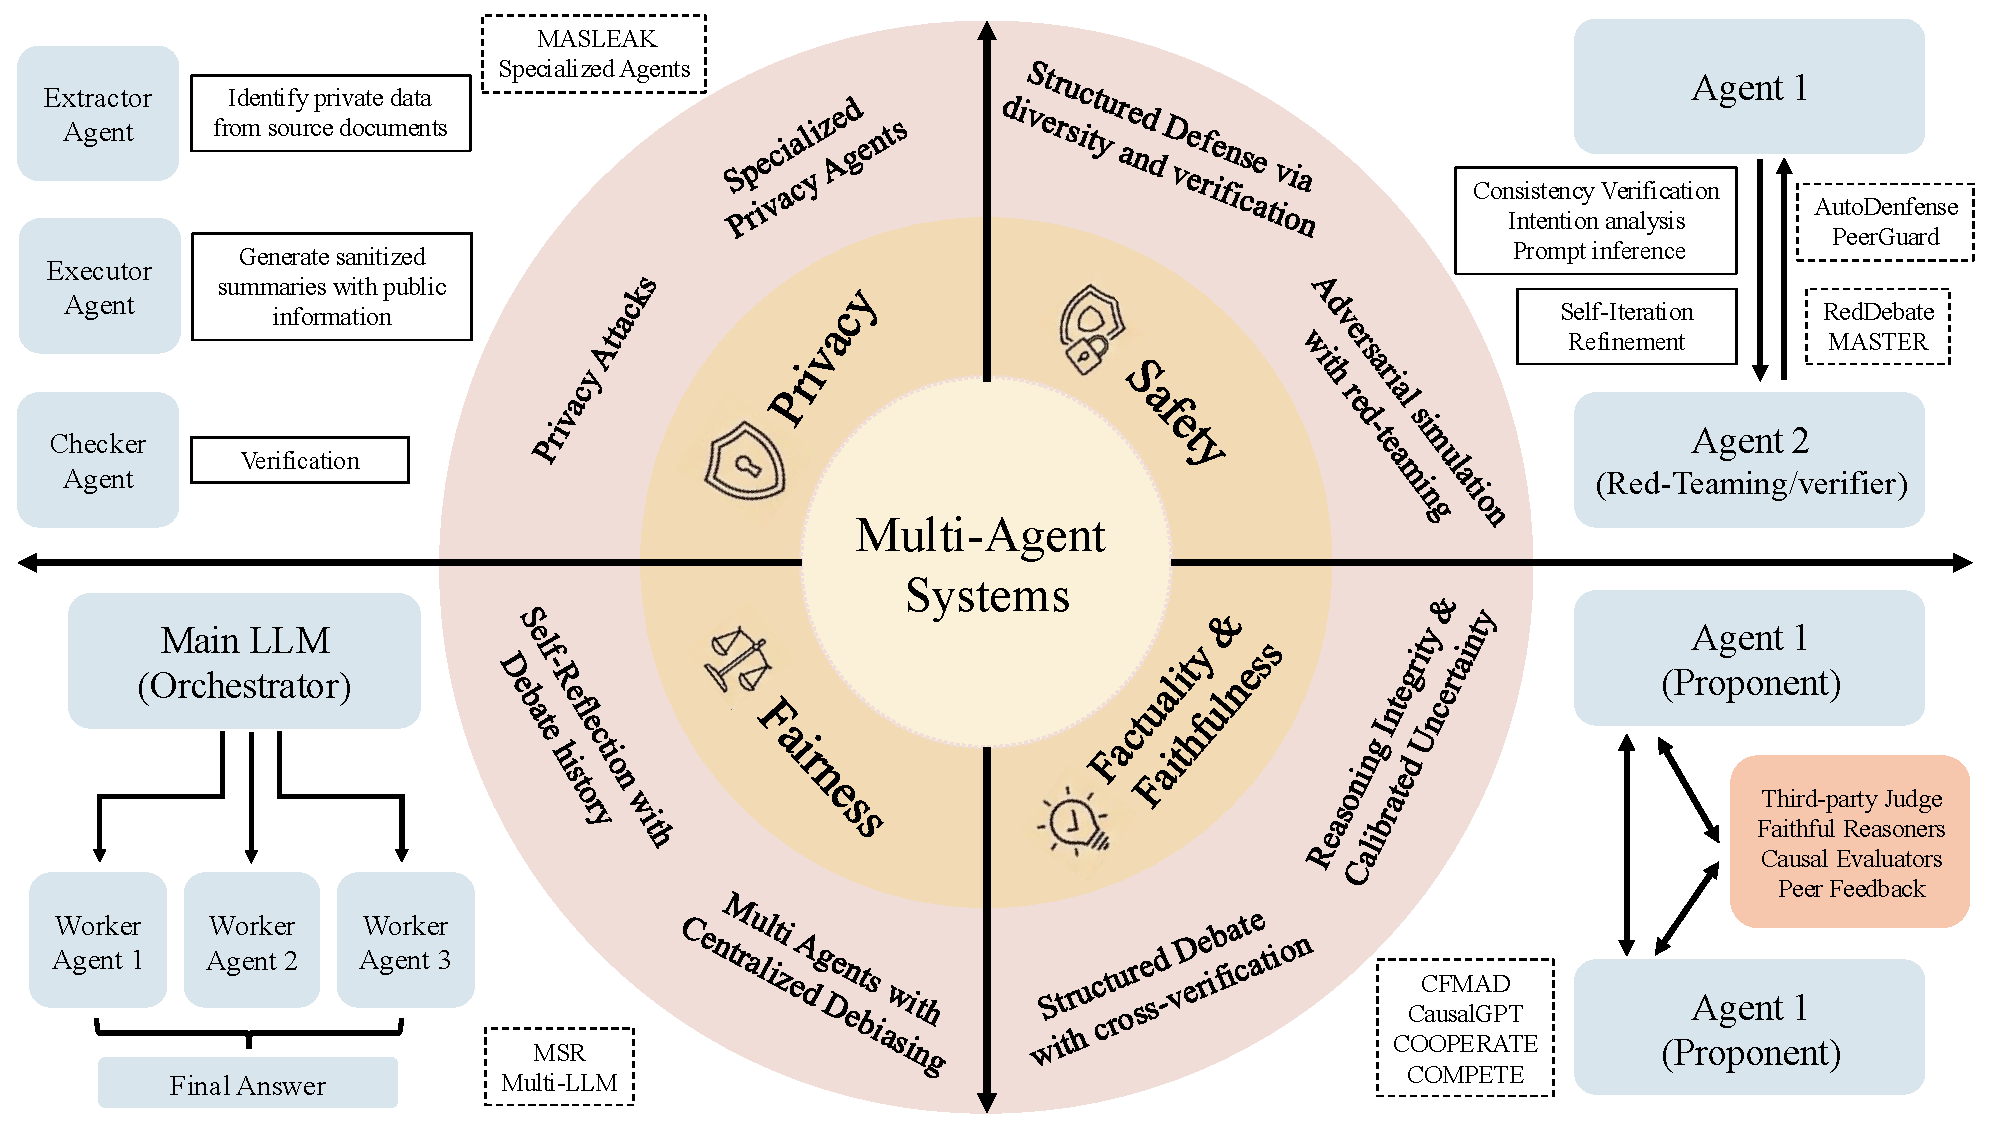
\includegraphics[width=0.9\linewidth]{figures/method/multi_agent.pdf}
  \caption{Overview of multi-agent system architectures for LLM trustworthiness across four dimensions. Safety employs structured defense via role diversity and adversarial red-teaming; Factuality relies on structured debate with cross-verification and calibrated uncertainty; Fairness uses multi-agent debiasing with self-reflection as well as orchestrated plan-and-refine loops; and Privacy leverages specialized agents (Extractor, Executor, Checker) for data sanitization. Representative systems and interaction patterns are shown for each dimension.}
  \label{fig:method_multiagent}
\end{figure*}

\subsubsection{Applications}
\paragraph{Safety}

Multi-agent systems turn safety from a static, single-model property into an emergent outcome of \emph{structured interaction}. Instead of relying on one model's filter, MAS instantiate a propose--attack--audit--adjudicate loop: specialized agents generate responses, probe for failures, cross-check reasoning, and arbitrate outcomes. A unifying pattern is \emph{structured defense via role diversity and cross-verification}. Systems like AutoDefense orchestrate intention analysis, prompt inference, and final judgment to filter unsafe outputs~\citep{zeng2024autodefense}. Committee-style analyzers extend coverage by combining linguistic, comment, and fact-checking expertise for misinformation risks~\citep{li2025multiagentframeworkautomateddecision}. Peer-based scrutiny hardens internal logic: PeerGuard has agents verify consistency between each other's chain-of-thought and final outputs to expose backdoors~\citep{fan2025peerguarddefendingmultiagentsystems}. At system scale, collaboration can be modeled as a temporal interaction graph to trace and arrest the spread of hallucinations or injected errors~\citep{zhou2025guardiansafeguardingllmmultiagent}, and dynamic credibility weighting further down-ranks unreliable contributors~\citep{ebrahimi2025adversaryresistantmultiagentllmcredibility}. Safety also benefits from \emph{adversarial simulation for proactive discovery}: automated red-teaming with debate has agents iteratively elicit, refine, and then patch unsafe behaviors using persistent memory~\citep{asad2025reddebatesaferresponsesmultiagent}. However, the same interactive channels expand the attack surface---structured debates can amplify jailbreak success~\citep{qi2025amplifiedvulnerabilitiesstructuredjailbreak}, communication links invite Agent-in-the-Middle manipulation~\citep{he-etal-2025-red}, persuasive agents can steer group consensus toward unsafe actions~\citep{zhang-etal-2024-psysafe}, and comprehensive security taxonomies such as MASTER map these vulnerabilities~\citep{zhu2025mastermultiagentsecurityexploration}, and broader analyses of \emph{emergent social risks} reveal how misaligned agent interactions can produce system-level harms that no individual agent was designed to cause~\citep{huang2026emergent}.

\paragraph{Factuality}

Multi-agent systems enhance factuality and faithfulness by replacing a single model's unverified reasoning with structured interaction among diverse agents. Rather than trusting one model's first-pass answer, MAS organize a propose--critique--adjudicate loop in which agents advance claims, attack each other's reasoning, and converge under a judge. Foundational work shows that debating agents can reach more accurate conclusions than individuals, as critiques expose faulty logic that a single model may miss~\citep{10.5555/3692070.3692537}, and debates judged by weaker raters still tend to favor truthful arguments~\citep{10.5555/3692070.3693020}. Forced-disagreement variants such as CFMAD assign counterfactual stances to improve robustness to initial mistakes~\citep{conf/coling/0008L0HF25}. This pattern scales to long-form tasks by decomposing outputs into atomic claims and verifying each through coordinated agents, including role-structured stateful debates~\citep{10889448}, discriminative reranking pipelines~\citep{wan-etal-2025-mamm}, complementary-perspective feedback for explanation faithfulness~\citep{kim2024llmsproducefaithfulexplanations}, and domain-specific evidence cross-examination~\citep{song2024auditllmmultiagentcollaborationlogbased}. Beyond surface correctness, MAS can promote reasoning integrity through separating faithful reasoners from causal evaluators~\citep{tang2025causalgptmultiagentapproachfaithful}, and calibrated uncertainty through peer feedback and adversarially generated alternatives that reveal knowledge gaps and trigger abstention~\citep{feng-etal-2024-dont, yang2024confidencecalibrationrationalizationllms}.

\paragraph{Fairness}
Multi-agent systems offer a promising path toward adaptively resolving complex biases across generation tasks, addressing demographic biases embedded in language patterns that simpler mitigation methods cannot effectively handle. A key direction is leveraging multi-agent debate to improve cultural adaptability:~\citet{ki-etal-2025-multiple} propose a framework where multiple LLM agents approach culturally situated questions through a mixture of debate and self-reflection actions, with a judge LLM resolving disagreements based on debate history. For demographic fairness, multi-agent architectures decompose the debiasing task across specialized roles: Mitigation via Selective Rewrite uses an LLM agent to provide targeted feedback on removing gender bias in language style~\citep{wan-chang-2025-white}, multi-LLM frameworks incorporate multiple models in conversational settings with both centralized and decentralized debiasing configurations~\citep{owens2024multi}, and self-reflection mechanisms enable models to identify and self-correct societal biases through a critique step~\citep{borah-mihalcea-2024-towards}.
Most recently, ~\citet{wan2025culturallensmodelsadopt} proposes an agentic planning pipeline with high autonomy, which orchestrates an iterated diagnose-and-refine loop until model generation reaches a satisfactory state.

\paragraph{Privacy}

While multi-agent systems introduce powerful mechanisms for safety and factuality, they also create novel privacy challenges representing a significant research gap. The interconnected nature of MAS establishes new vectors for data leakage: the MASLEAK framework demonstrates systematic, worm-like attacks that can extract high-value intellectual property such as system prompts, tool definitions, and topological structure from black-box MAS applications by propagating through agent communication chains~\citep{wang2025ipleakageattackstargeting}. Conversely, the same architectural principles can be leveraged for defense: multi-agent approaches decompose the complex task of privacy preservation into specialized roles---such as an Extractor Agent to identify private data, an Executor Agent to generate sanitized outputs, and a Checker Agent for verification---significantly reducing leakage of sensitive information while preserving output quality~\citep{li-etal-2025-1}. These studies highlight a critical duality where the collaborative structure of MAS is both a liability and an asset for privacy, though a holistic understanding encompassing robust defenses, secure communication protocols, and verifiable information-flow controls remains largely unexplored.


% --- Evaluation, Challenges, Conclusion ---
\section{Evaluation}
\label{sec:evaluation}

Inference-time trustworthiness methods intervene after model training to shape LLM behavior under deployment constraints. As these interventions differ a lot in where and how they act, such as in prompts, logits, activations, external filters, or the system workflow, evaluation cannot be unified by one benchmark or one metric family. Although foundational benchmarks such as TrustGPT~\citep{huang2023trustgpt} and dynamic evaluation toolkits such as TrustEval~\citep{wang2025trusteval} provide valuable unified views over multiple trustworthiness dimensions, they were not designed to isolate the runtime-specific properties introduced by inference-time controls. We therefore adopt a meta-axis evaluation view on the inference-time evaluation. The goal is to capture deployment-relevant properties that arise specifically from runtime trustworthiness. In practice, such enforcement is shaped by latency, cost, and integration constraints. Each axis highlights a distinct evaluation question, and while the axes are conceptually unique, they can overlap in practice:

\begin{figure*}[htbp]
  \centering
  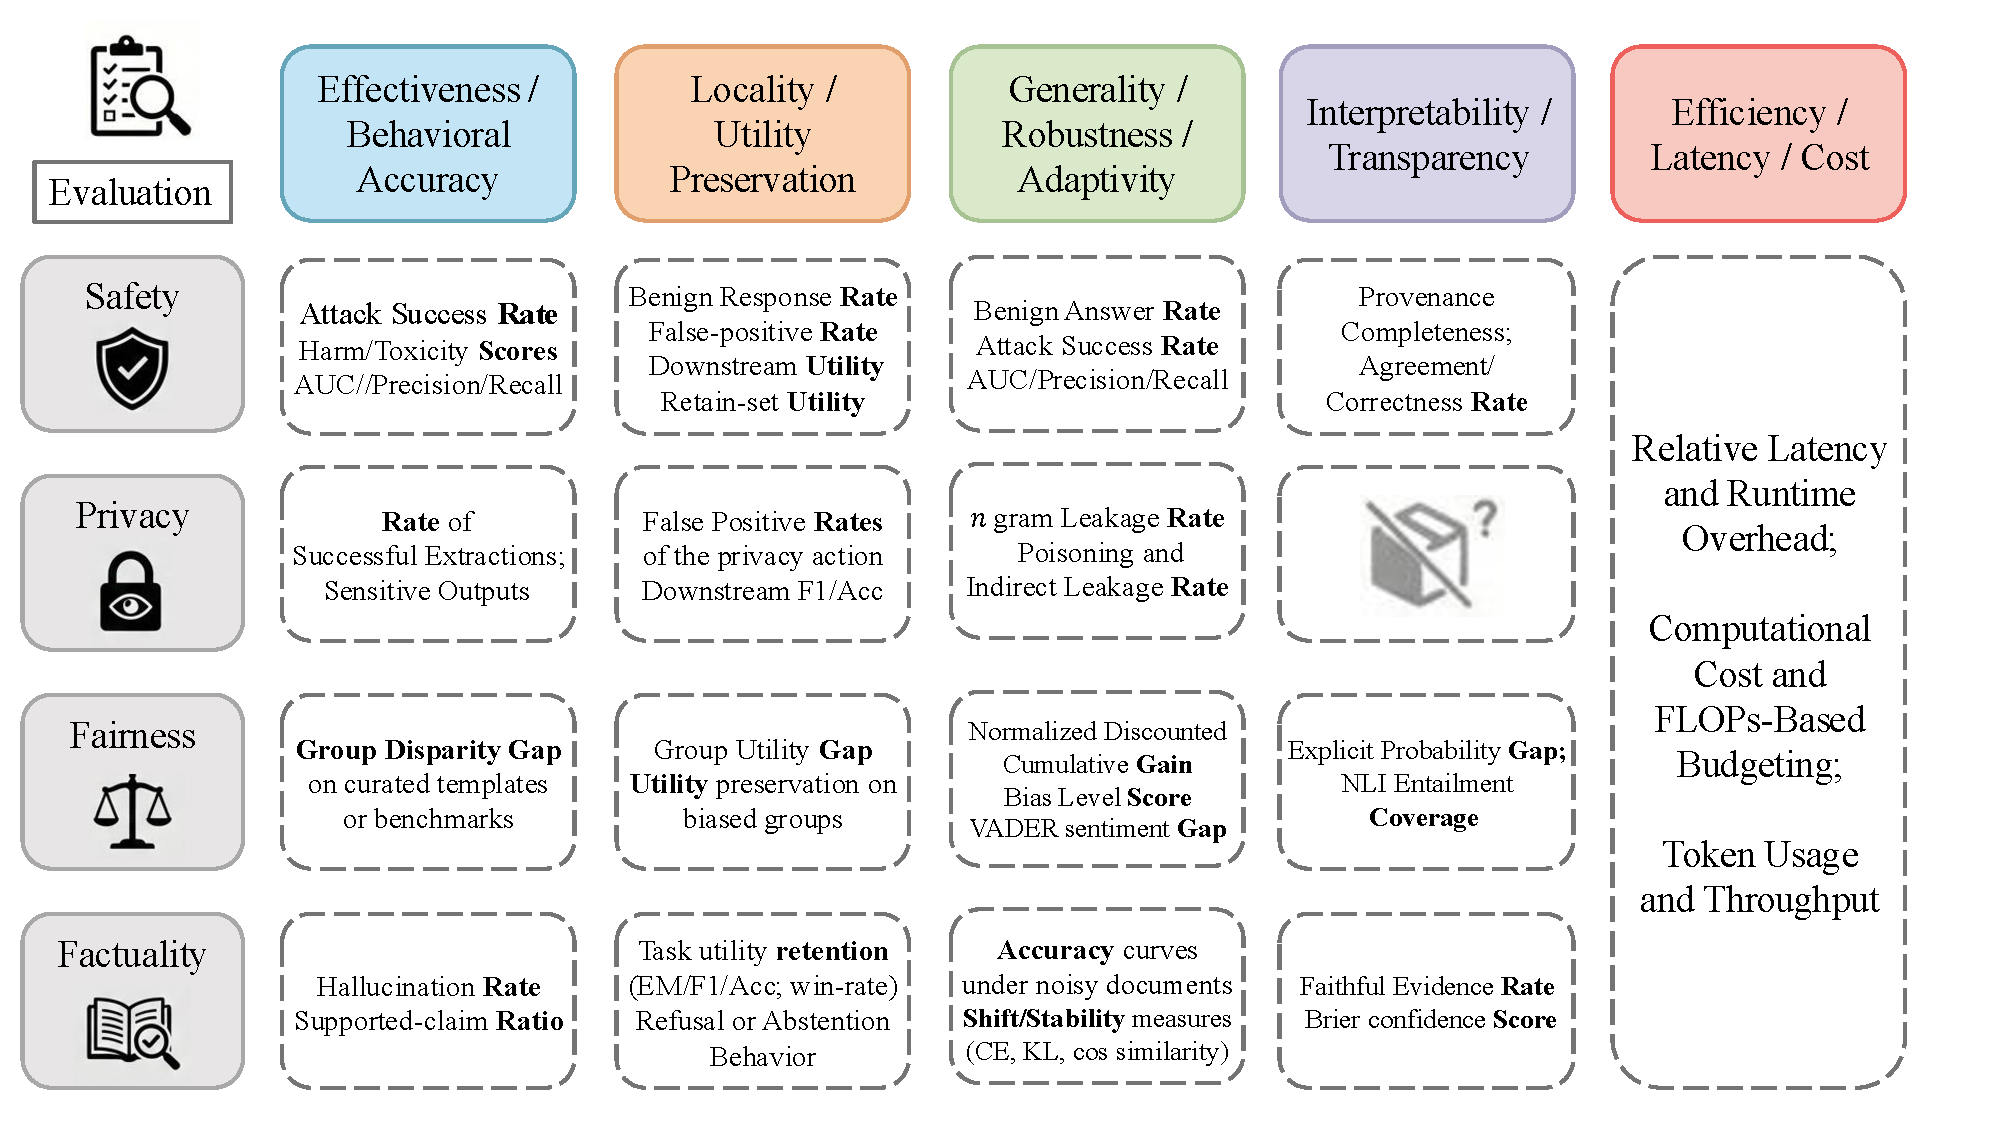
\includegraphics[width=0.9\linewidth]{figures/method/evaluations.pdf}
  \caption{A meta-axis evaluation framework for inference-time trustworthiness methods. Rows correspond to four trustworthiness dimensions (Safety, Privacy, Fairness, Factuality), and columns represent five complementary evaluation axes (Effectiveness, Locality, Generality, Interpretability, Efficiency). Each cell lists representative metrics specific to the dimension--axis intersection, highlighting the multi-faceted nature of deployment-time evaluation.}
  \label{fig:evaluation}
\end{figure*}

\begin{itemize}
\item \textbf{Effectiveness / Behavioral Accuracy}: To what extent does the inference-time mechanism reliably enforce the intended behavioral constraints, and under what conditions does it fail?
\item \textbf{Locality / Utility Preservation}: To what extent are the intervention effects localized to the targeted behaviors while preserving general task performance and user utility?
\item \textbf{Generality / Robustness / Adaptivity}: How well does the mechanism generalize across tasks, domains, and input distributions, and how robust is it to distributional shifts?
\item \textbf{Efficiency / Latency / Cost}: What additional runtime overhead does the mechanism introduce in terms of latency, compute, memory, or token usage?
\item \textbf{Interpretability / Transparency}: To what extent are the mechanism’s actions, triggers, and decision rationales transparent to human auditors or downstream systems?
\end{itemize}

Although these axes separate different deployment concerns, they often trade off against one another. 
% For example, a guardrail detector may score highly on effectiveness, such as achieving a high AUC, yet still fail on locality by excessively blocking benign content. Similarly, a method can succeed on safety under standard conditions but fail on robustness when it is bypassed by prompt injection.
Building on this framing, this section organizes evaluation along the axes above and surveys representative metrics, across four categories: Safety, Privacy, Fairness, and Factuality.

\subsection{Effectiveness / Behavioral Accuracy}
Effectiveness / Behavioral Accuracy evaluates whether an inference-time mechanism $\mathcal{M}$ changes model behavior in the intended direction on a target evaluation distribution. Consider an LLM that produces an output $Y_{\mathcal{M}}(x)$ for an input $x \sim \mathcal{D}$ under $\mathcal{M}$. Effectiveness asks whether $\mathcal{M}$ increases the likelihood of desired trust-aligned behavior and decreases the likelihood of undesired behavior:
\[
\text{Effectiveness}(\mathcal{M}) \propto
\mathbb{E}_{x \sim \mathcal{D}}
\Big[
\mathbf{1}\{Y_{\mathcal{M}}(x)\in \mathcal{Y}_{\text{desired}}\}
-
\mathbf{1}\{Y_{\mathcal{M}}(x)\in \mathcal{Y}_{\text{undesired}}\}
\Big].
\]
In inference-time settings, this axis primarily measures the runtime behavior induced by a plug-in control layer, such as refusal, redaction, constrained decoding, evidence grounding, or verification. However, Effectiveness alone does not tell whether improvements come from overly broad suppression of benign behavior, from brittle operating thresholds, or from masking the underlying capability. These trade-offs motivate complementary axes such as Locality (utility and over-refusal), Robustness (bypassability and shift), Efficiency (latency/cost), and Interpretability (auditability).

\subsubsection{Rate-Based Metrics}
Rate-based metrics capture how often undesired behavior still occurs at inference time, and are the most prevalent family across all trustworthiness categories. In safety, jailbreak success rate measures whether an adversarial prompt elicits a harmful response from the model, unsafe completion rate tracks the overall proportion of harmful outputs across all queries, and the complementary defense success rate captures how often the mechanism successfully blocks such outputs. Risk-score formulations take a continuous toxicity or harm score assigned to each output instead of a binary attack outcome and report the fraction exceeding a predefined threshold~\citep{kumar2024certifying, Xu2024SafeDecodingDA, Huang2024SafeAlignerSA, chen2025safeptr, deng2025guard, hasan2024pruning, fan2025peerguarddefendingmultiagentsystems, yan2025dual}. In privacy, extraction success rate captures whether an attacker can recover memorized or sensitive text from model outputs, while disclosure rate measures how often outputs contain personally identifying or otherwise private information across a broader query distribution~\citep{pawelczyk2023context, Borec2024TheUI, Wang2025PrivacyAwareDM, zou2025poisonedrag}. In factuality, hallucination rate counts the proportion of outputs that are unsupported or factually incorrect, groundedness rate measures the fraction of claims in a response that are explicitly supported by retrieved or provided evidence, and edit success rate verifies whether a targeted fact has been correctly updated following a knowledge editing intervention~\citep{dhuliawala2024chain, asai2024self, zhou2024metacognitive, meng2022locating, meng2022memit}.

\subsubsection{Classifier-Style Metrics}
Classifier-style metrics treat the inference-time intervention as an explicit detection task and evaluate how well the mechanism separates harmful, private, or hallucinated outputs from benign ones. Rather than reporting a single operating point, metrics such as AUC and AUPRC summarize performance across all possible decision thresholds, while Precision, Recall, and F1 show the trade-off between false positives and false negatives at a chosen threshold. These metrics are important when the intervention involves a learned or rule-based classifier, such as a safety guardrail or hallucination detector, where threshold calibration governs deployment behavior. They appear across safety guardrails~\citep{Padhi2024GraniteG, Chi2024LlamaG3, Kumar2025PolyGuardAM, Liu2025GuardReasonerTR}, privacy membership-inference evaluations~\citep{zou2025poisonedrag, nakka2025piijailbreaking}, and factuality hallucination detection~\citep{asai2024self, zhou2024metacognitive}.

\subsubsection{Group-Disparity Metrics}
Group-disparity metrics quantify fairness effectiveness by comparing outcomes across demographic groups, capturing whether a mechanism treats different populations equitably. Bias scores on curated benchmarks measure stereotyping or differential toxicity for specific groups, worst-group performance identifies the most disadvantaged subpopulation, and disparity gaps capture the absolute difference in an outcome metric such as toxicity, error rate, or refusal rate between two groups. Together, these metrics reveal whether a fairness intervention reduces imbalance in model behavior or merely shifts it. They are reported across prompt-based interventions~\citep{dwivedi2023breaking, huang2024bias, kamruzzaman2024prompting}, fairness-aware retrieval~\citep{chen2024spica, shrestha2024fairrag}, and pruning methods that target bias-related internal structure~\citep{cai2024locating, zayed2024fairness, ma2025breaking}.

\subsubsection{Task-Performance Metrics}
Task-performance metrics such as exact match, F1, and accuracy measure whether trustworthiness gains come at the cost of general capability, serving as a sanity check on standard benchmarks. They are widely reported among representation or context engineering evaluations to confirm that they do not disrupt unrelated competencies~\citep{li2023iti, bayat2024enhanced, wang2024act, meng2022locating}, and also appear in multimodal hallucination settings~\citep{Park2024ConVisCD, Yuan2024HELPDMH}.

% Across all four categories, a low failure rate does not imply a better system if it results from an overly conservative operating point that suppresses benign requests, and task-accuracy gains can be confounded by format changes or benchmark saturation. Effectiveness metrics should therefore always be interpreted alongside Locality, Robustness, and Interpretability evaluations.

\subsection{Locality / Utility Preservation}
Locality / Utility Preservation evaluates whether an inference-time mechanism $\mathcal{M}$ limits its behavioral changes to the intended outputs while preserving user utility. Unlike training-time alignment, inference-time controls are typically implemented as plug-in layers. As a result, the locality failure mode is behavioral spillover, in which the system becomes safer by being less helpful, issuing more refusals, or providing less information. Formally, let $\mathcal{D}_{\text{tgt}}$ denote the targeted distribution (e.g., harmful or sensitive prompts) and $\mathcal{D}_{\text{benign}}$ denote benign traffic. A generic utility retention view is:
\[
\Delta U_{\text{benign}}(\mathcal{M})
=
\mathbb{E}_{x\sim \mathcal{D}_{\text{benign}}}\!\left[u\!\left(Y_{\mathcal{M}}(x)\right) - u\!\left(Y(x)\right)\right],
\]
where $u(\cdot)$ can be task accuracy (EM/F1/Acc), LLM-as-judge helpfulness, or win-rate. In inference-time deployment, locality is coupled to thresholding and pipeline composition. When multiple strategies are combined, such as guardrails and decoding, they can amplify suppression of benign outputs even if each component appears acceptable in isolation.


\subsubsection{False-Positive and Over-Refusal Rate Metrics}
These metrics capture whether a mechanism incorrectly suppresses or refuses inputs it was not designed to target. In safety, benign response rate measures how often the defense leaves safe prompts unaffected, and is usually reported alongside attack success rate to confirm that refusal gains are not simply the result of refusing more broadly~\citep{kumar2024certifying, cao2024defending, ji2024defending, zhou2024defending}. In guardrail systems, false-positive rate and benign blocking rate capture how often clean inputs are incorrectly filtered or routed. These summarize the trade-off between blocking harmful content and passing benign traffic~\citep{Padhi2024GraniteG, Chi2024LlamaG3, Kumar2025PolyGuardAM, Liu2025GuardReasonerTR}. In multi-agent defenses, false alarm rates on clean interactions are essential because a monitoring agent that incorrectly flags benign exchanges can suppress the entire downstream workflow~\citep{fan2025peerguarddefendingmultiagentsystems, asad2025reddebatesaferresponsesmultiagent}. In privacy, false positives of the privacy action through blocking harmless queries, measure damage on non-sensitive content~\citep{pawelczyk2023context, Wang2025PrivacyAwareDM}. In fairness, refusal disparity measures the absolute difference in refusal rate between demographic groups under the intervention, capturing whether the mechanism disproportionately suppresses responses for certain groups rather than improving equitable helpfulness~\citep{dwivedi2023breaking, huang2024bias, kamruzzaman2024prompting}.

\subsubsection{Utility Retention Metrics}
Utility retention metrics measure whether general task performance is preserved on non-targeted inputs after the intervention. Common metrics include exact match, F1, and accuracy on held-out benchmarks, MT-Bench scores, instruction-following rates, LLM-as-judge helpfulness, and win-rate. In safety, these are reported for decoding, representation engineering, pruning, and unlearning interventions to confirm that modifications do not distort normal generation quality~\citep{Xu2024SafeDecodingDA, Arditi2024SingleDirection, chen2025safeptr, hasan2024pruning, deng2025guard, zhang2024theft}. In privacy, downstream task accuracy on non-sensitive queries confirms that filtering or constrained generation does not broadly reduce answer quality~\citep{Borec2024TheUI, zou2025poisonedrag}. In fairness, per-group utility retention tracks whether task success is preserved equitably across demographic groups, ensuring bias reduction is not obtained by broadly degrading helpfulness for any subpopulation~\citep{shrestha2024fairrag, cai2024locating, zayed2024fairness, ma2025breaking}. In factuality, retain-set task utility on benign factual QA is reported alongside hallucination reductions~\citep{dhuliawala2024chain, li2023iti, asai2024self, zhou2024metacognitive}.

\subsection{Generality / Robustness / Adaptivity}
Generality / Robustness / Adaptivity evaluate whether an inference time mechanism $\mathcal{M}$ keeps its intended effect when inputs, tasks, or attackers change at deployment. This axis is not about a single test set. It is about performance over a family of conditions, which is likely out-of-distribution. Let $\{\mathcal{D}_k\}_{k=1}^K$ be test distributions and let $s_k(\mathcal{M})$ be a score on $\mathcal{D}_k$. A common summary reports both the average and the worst case:
\[
s_{\mathrm{avg}}(\mathcal{M})=\frac{1}{K}\sum_{k=1}^K s_k(\mathcal{M}),
\qquad
s_{\min}(\mathcal{M})=\min_{k\in[K]} s_k(\mathcal{M}).
\]
% In inference-time settings, $s_{\min}$ is often more critical for deployment because the system must handle rare but high-risk inputs.

\subsubsection{Worst-Case and Cross-Distribution Rate Metrics}
These metrics summarize how a mechanism's core effectiveness signal holds up across multiple conditions rather than a single fixed distribution. In safety, attack success rate and benign answering rate are reported across multiple jailbreak families and prompt styles, with worst-case values serving as the primary robustness summary. Sensitivity to threshold changes is captured by reporting deltas when guard strength varies~\citep{kumar2024certifying, cao2024defending, zhou2024defending}. Decoding and representation engineering methods report harmful score and safety score under stronger or more diverse attacks. Tracking utility accuracy on task suites to confirm that robustness gains do not come at the cost of normal performance~\citep{Xu2024SafeDecodingDA, Wang2024InferAligner, deng2025guard}. In privacy, attack success rate is reported across multiple attack types and privacy budgets to capture how leakage behavior changes as the adversary changes. N-gram leakage rate measures whether the control generalizes beyond exact span matches to broader overlap with sensitive content~\citep{tong2025inferdpt, chaudhari2024phantom}. In fairness, bias scores and stereotype index are reported across demographic categories, topics, and occupations to evaluate whether bias reduction holds beyond a fixed template. Fairness violation rates are tracked alongside utility metrics such as NDCG~\citep{kamruzzaman2024prompting, dwivedi2023breaking, huang2024bias}. In factuality, accuracy and F1 are reported across cross-domain splits to test whether robustness comes from better evidence selection rather than longer contexts~\citep{wan2024dell, dhuliawala2024chain, zhou2024metacognitive, asai2024self}.

\subsubsection{Classifier-Style Metrics Across Domains and Languages}
When the intervention involves an explicit detector or classifier, robustness is evaluated by reporting precision, recall, F1, AUC, and AUPRC across multiple benchmarks, domains, and languages. In safety, guardrails and multi-agent systems use these metrics to evaluate whether detection quality generalizes across domains and languages~\citep{Padhi2024GraniteG, Ghosh2024AEGISOA, asad2025reddebatesaferresponsesmultiagent}. In privacy, precision, recall, and F1 for detecting poisoned passages evaluate whether the control generalizes to different poisoning strategies, since both false positives and false negatives matter~\citep{zou2025poisonedrag, zhong2023poisoning}. In fairness, detailed metrics such as sentiment gap, toxicity scores, and regard-based labels are reported across demographic groups to evaluate how robust the fairness conclusion is to different measurement approaches~\citep{zayed2024fairness, dasu2025attention}.

\subsubsection{Calibration and Stability Metrics}
These metrics evaluate whether a mechanism remains consistent and reliable as conditions shift. In safety, expected calibration error tests whether the same decision threshold remains reliable under distribution shift. In factuality, representation engineering methods track shift measures such as cross-entropy and KL divergence to detect distribution change, and stability measures such as cosine similarity to check whether the intervention direction stays consistent as training data changes~\citep{li2023iti, zou2023representation, bayat2024enhanced}. In fairness, cross-split and cross-capability comparisons, reporting generality scores on train-test splits, check whether bias reductions are stable rather than artifacts of a particular evaluation setup~\citep{qin2024mitigating, cai2024locating}.


\subsection{Interpretability / Transparency}
Interpretability / Transparency evaluates whether an inference-time mechanism $\mathcal{M}$ is observable and auditable. When $\mathcal{M}$ changes the system behavior (e.g., refusal, redaction, or rewriting), it should be clear (i) what action was taken, (ii) what condition triggered the action, and (iii) what evidence supports the decision. This is particularly important at inference time because many controls are deployed as modular plug-ins. Formally, let $a_{\mathcal{M}}(x)\in\mathcal{A}$ denote the runtime action on input $x$, and let $\tau_{\mathcal{M}}(x)$ be the trigger set (policy IDs, detectors, or threshold crossings). Let $z_{\mathcal{M}}(x)$ be the transparency artifact (logs, scores, or traces). A generic transparency score is:
\[
T(\mathcal{M})
=
\mathbb{E}_{x\sim\mathcal{D}}
\left[
v\!\left(a_{\mathcal{M}}(x),\, \tau_{\mathcal{M}}(x),\, z_{\mathcal{M}}(x)\right)
\right],
\]
where $s(x)$ is a risk score (or classifier confidence) and $t$ is the deployed threshold.


\subsubsection{Provenance and Audit Metrics}
These metrics measure whether each intervention is accompanied by a sufficient audit record that identifies what component acted, what policy triggered it, and at what operating point. In safety, provenance completeness captures whether each intervention includes a stage identifier, policy identifier, risk score, and threshold value, making it possible to distinguish targeted filtering from broad over-refusal~\citep{song2024auditllmmultiagentcollaborationlogbased, zhou2025guardiansafeguardingllmmultiagent, Liu2025GuardReasonerTR, chen2025safeptr}. In factuality, provenance logs of what was retrieved and used at runtime help separate retrieval failures from generation failures, and verification loops or critique-style retrieval augmentation leave intermediate records that make the reasoning process auditable~\citep{dhuliawala2024chain, asai2024self, wan2024dell}.

\subsubsection{Human Judgment Metrics}
These metrics evaluate whether the mechanism's explanations are understandable to human annotators. In safety, agreement rate measures the fraction of explanations that annotators judge as correct or helpful, evaluating whether intermediate reasoning steps and policy triggers are meaningful rather than superficially plausible~\citep{ji2024defending, Kang2024R2GuardRR}. In factuality, faithful explanation rate measures the fraction of explanations that humans consider consistent with the provided evidence, evaluating whether verification rationales are genuinely grounded~\citep{kim2024llmsproducefaithfulexplanations, asai2024self}. LLM-as-a-judge is widely used as a scalable proxy for human judgment, but recent work shows that judge models themselves carry systematic biases---e.g., position, verbosity, and self-preference biases---which can distort transparency evaluations and should be reported alongside raw judge scores~\citep{ye2024justice}.

\subsubsection{Distributional Transparency Metrics}
These metrics evaluate whether the mechanism's behavior across groups or confidence levels is auditable from the output distribution. In fairness, an explicit probability gap between two matched identity terms in the same context measures how much the mechanism shifts likelihoods across groups~\citep{cai2024locating}. In pluralistic settings, NLI entailment coverage measures how much the final response reflects provided group viewpoints, capturing whether the mechanism genuinely incorporates intended perspectives~\citep{qin2024mitigating}. In factuality, calibration metrics such as the Brier score measure whether reported confidence aligns with actual correctness, making the system's factuality claims auditable across varying operating points~\citep{10.5555/3692070.3693020, yang2024confidencecalibrationrationalizationllms}. 
% A shared concern is that distributional scores can be misleading at a single operating point: changing a threshold or retrieval rule can shift group coverage or confidence distributions, so scores should be reported across multiple operating points rather than at a fixed setting.

\subsection{Efficiency / Latency / Cost}
Efficiency / Latency / Cost evaluates how practical it is to deploy an inference-time mechanism $\mathcal{M}$ by measuring the computational resources consumed during the control process. Unlike training-time alignment, which spreads costs over the model's lifetime, inference-time methods operate on the critical path of user interaction. Even small increases in latency or compute per request can noticeably worsen user experience and raise operational costs. The main efficiency failure mode is excessive overhead, where the mechanism requires many extra forward passes, memory, or auxiliary calls to achieve safety or accuracy improvements. Formally, let $C_{\text{base}}(x)$ denote the cost of generating a response for input $x$ using the base model. A general overhead measure is:
\[
\Delta C(\mathcal{M})
=
\mathbb{E}_{x\sim \mathcal{D}}\!\left[ C_{\mathcal{M}}(x) - C_{\text{base}}(x) \right],
\]
where $C_{\mathcal{M}}(x)$ is the cost under the mechanism. The commonly used metrics are:
\begin{itemize}
    \item \textbf{Relative Latency and Runtime Overhead.}
    A standard way to measure deployment cost is relative latency, often reported as the \textit{Average Token Generation Time Ratio} or its equivalence~\citep{Xu2024SafeDecodingDA, Liu2024AlignmentEnhancedDD, Li2024CleanGenMB}. It measures the slowdown caused by the defense during inference:
    \[
    \text{ATGR} = \frac{1}{N} \sum_{i=1}^{N} \frac{T_{\text{def}}(x_i)}{T_{\text{base}}(x_i)},
    \]
    where $T_{\text{def}}(x_i)$ is the wall-clock time for prompt $x_i$ under the defense, and $T_{\text{base}}(x_i)$ is the baseline time.
    \item \textbf{Computational Cost and FLOPs-Based Budgeting.}
    To study scaling behavior in a way that is less sensitive to hardware, several works use floating point operations as a compute proxy~\citep{qiu2025saffron, Lee2025SafeRouteAM}. This gives a hardware-independent view of how much extra computation is needed for a given safety gain, often reported as performance under a compute budget:
    \[
    \text{Performance}(C_{\text{budget}}) = \text{Metric}\!\left(\mathcal{M} \mid C_{\mathcal{M}} \le C_{\text{budget}}\right).
    \]
    This is used to plot safety outcomes such as Attack Success Rate against inference TFLOPs, tracing a safety--compute trade-off curve.
    \item \textbf{Token Usage and Throughput.}
    For methods that expand context---such as guardrail prompting, meta-prompting, or retrieval augmentation---token growth is a direct cost driver~\citep{Jiang2023POSTERIA, shrestha2024fairrag, Zeng2024RootDS}. A simple and widely used summary is the \textit{Token Usage Ratio}:
    \[
    r_{TT} = \frac{\text{Total Tokens}_{\text{defense}}}{\text{Total Tokens}_{\text{base}}}.
    \]
    This captures cost increases from longer prompts, extra intermediate steps, or additional retrieved content. Throughput in tokens per second is also commonly reported to reflect serving capacity under the defense.
\end{itemize}
\section{Open Challenges and Future Directions}
\label{sec:challenges}

% === Consolidated Discussion by Tier ===

\subsection{External Controls}

Context engineering, guardrails, and decoding strategies share a common strength: they treat the model as a black box, making them model-agnostic, composable, and rapidly updatable without retraining. Context engineering is training-free and flexible, with different techniques naturally addressing distinct challenges---prompting for lightweight alignment, RAG for factual grounding, memory for persistence, and reasoning for self-regulation. Guardrails add an independent policy-enforcement layer that can be swapped across providers, while decoding strategies enable fine-grained, real-time steering of token distributions across multiple trustworthiness dimensions.

However, all three tiers are fundamentally soft controls and share similar failure modes. Context engineering is fragile to small phrasing changes and vulnerable to context poisoning; guardrails face a continuous cat-and-mouse dynamic against adversarial evasion; and hard decoding constraints can produce brittle, incoherent outputs~\citep{Huang2024SafeAlignerSA}. A common ``Control Tax'' underlies these methods: strict guardrails increase false positives and reduce helpfulness, while aggressive logit suppression~\citep{Zhao2024AdversarialCD} or noise injection~\citep{Majmudar2022DifferentiallyPD} compromises generation quality. Complex LLM-based judges and multi-layer decoding further introduce significant latency overhead. None of these methods can provide formal safety guarantees in isolation, and integrated pipelines that combine context engineering, guardrails, and decoding remain underexplored.

\subsection{Internal Manipulations}

Representation engineering, unlearning, and pruning offer more direct behavioral control by intervening on internal model components. Representation engineering treats hidden states as controllable objects, enabling concept-level steering through activation addition or sparse autoencoders~\citep{zou2023representation,li2023iti,turner2023steering}. Unlearning steers outputs away from sensitive knowledge through runtime penalties or influence subtraction, making it practical for dynamic regulatory demands. Pruning provides structural control by removing heads, neurons, or tokens associated with unsafe or biased behavior, and is compatible with broader compression pipelines.

Despite these strengths, internal methods share key fragilities. Representation engineering depends heavily on intervention strength, layer choice, and normalization; multi-concept steering remains brittle, and strong interventions risk pushing activations out of distribution~\citep{wehner2025taxonomy}. Unlearning faces a fundamental verification problem: many methods suppress rather than truly remove knowledge, leaving models vulnerable to adversarial recovery~\citep{lucki2024adversarial}. Pruning is highly sensitive to where sparsity is introduced---even small amounts of naive pruning can sharply weaken safety-critical behavior. All three methods also exhibit a utility--control trade-off, where stronger interventions can degrade fluency, accuracy, or reasoning~\citep{liu2024breaking}. Additionally, representation engineering carries dual-use risks, as the same activation-level controls can strengthen or weaken safety~\citep{revisiting2025jailbreaking}. Robust deployment across internal methods will require better verification protocols, principled intervention selection, and careful integration with broader safety governance~\citep{nist2025ai8001}.

\subsection{System-Level Orchestration}

Multi-agent systems introduce reliability through collaborative reasoning, but their most immediate obstacle is operational overhead: each query may trigger multiple agents over several rounds, with performance gains often diminishing quickly~\citep{conf/coling/0008L0HF25, 10.5555/3692070.3692537}, rendering many architectures impractical for real-time applications~\citep{song2024auditllmmultiagentcollaborationlogbased}. Moreover, the collaborative dynamics designed to foster trustworthiness can become vectors for emergent failures. Agents sharing the same base model exhibit ``groupthink,'' reinforcing shared hallucinations~\citep{conf/coling/0008L0HF25}, and adversaries can exploit the collaborative structure---a single persuasive adversary can sway an entire group~\citep{amayuelas-etal-2024-multiagent}, while debate frameworks can be more vulnerable to jailbreaks than single agents~\citep{qi2025amplifiedvulnerabilitiesstructuredjailbreak}. Evaluating MAS trustworthiness is also fundamentally more complex, as effectiveness depends on roles, topology, protocols, and agent count~\citep{zhu2025mastermultiagentsecurityexploration}.


%%%%%%%%%%%%%%%%%%% Original Disucssion (DO NOT TOUCH)%%%%%%%%%%%%%%%%%%%
% \textcolor{blue}{Below are original Discussion Section}
% The inference-time methods surveyed in this work represent a paradigm shift towards dynamic, modular, and accessible control over LLM behavior. While promising, their widespread adoption is hindered by fundamental challenges that cut across the entire taxonomy. Moving from ad-hoc interventions to a robust engineering discipline for trustworthiness requires a concerted research effort focused on overcoming the fragility of controls, managing performance trade-offs, developing scalable solutions, and understanding system-level effects. We synthesize these challenges into a forward-looking research agenda.

% \paragraph{Overcoming the Brittleness of Controls}
% A recurring theme is the fragility of inference-time interventions. Controls are often highly sensitive to minor variations in input or model state, leading to unpredictable failures. Context engineering, for instance, is notoriously fragile, where slight rephrasing can bypass safety instructions. This brittleness extends to internal methods; knowledge editing has revealed that LLMs are highly fragile to weight perturbations, where localized edits can cause catastrophic degradation of general abilities. Similarly, representation engineering struggles with fragile generalization, as steering effects can be inconsistent across different layers or generation lengths, while hard constraints in decoding strategies can lead to brittle and incoherent outputs. Future work must move beyond controls that work only under narrow conditions. This necessitates developing methods for \textit{robustification}, potentially through adversarial training of the control mechanisms themselves, to ensure they generalize across a wider distribution of inputs and contexts.

% \paragraph{Quantifying and Mitigating the Control Tax}
% Nearly every method introduces a trade-off between trustworthiness and utility, a phenomenon that can be termed a "Control Tax." Imposing stricter controls on model behavior often degrades core performance metrics like fluency, accuracy, and helpfulness. This is explicit in guardrails, which must balance safety and helpfulness, and in decoding strategies, which face a direct trade-off between control strength and generation quality. The tension is also evident in unlearning methods, where achieving stronger unlearning efficacy often harms model utility, and in pruning, where removing components for safety can cause collateral damage to general capabilities. A primary goal for future research should be to formally understand and quantify this Control Tax. This requires creating standardized benchmarks that explicitly measure performance across a joint distribution of task-based and trust-based metrics, with the ultimate aim of designing new methods that push the Pareto frontier, minimizing the utility penalty required to achieve a desired level of trust.

% \paragraph{Addressing the Scalability and Efficiency Barrier}
% For inference-time methods to be practical, they must be computationally efficient. Several powerful techniques, however, impose significant overhead in latency and cost, creating a "viability barrier" for real-world deployment. Multi-agent systems are a primary example, as their multiplicative demand for LLM calls renders them impractical for most real-time applications. Similarly, complex guardrails, particularly those using an LLM-as-a-judge, introduce noticeable latency that is unacceptable in many user-facing scenarios. Even advanced decoding strategies can introduce computational overhead at each generation step. The field therefore needs a greater focus on lightweight and efficient control mechanisms. Promising directions include distilling the behavior of complex MAS or judge models into smaller, faster classifiers and developing pruning techniques that are aligned with hardware acceleration to achieve speedups without compromising trustworthiness.

% \paragraph{Defending Against Adaptive Adversaries}
% Many current methods are static defenses vulnerable to adaptive adversaries who continuously discover new bypass techniques. This creates a reactive "cat-and-mouse" dynamic, where developers are constantly patching vulnerabilities. Guardrails are often susceptible to adversarial evasion, and unlearning methods can be circumvented by adversarial probing that recovers supposedly erased information. More complex systems are not immune; multi-agent systems can be manipulated by a single persuasive adversary and have been shown to be more vulnerable to certain jailbreaks than single models. Future work must therefore shift from static defenses to dynamic, adaptive security postures. This involves developing methods for real-time threat detection, automated red-teaming to discover vulnerabilities proactively, and control systems that can adapt their strategies in response to detected attacks.

% \paragraph{The Unsolved Problems of Generalization and Composition}
% A critical limitation of many targeted interventions is their failure to generalize. Furthermore, how different inference-time methods interact when layered together remains poorly understood. Knowledge editing exemplifies the generalization challenge, where an edit often fails to transfer to rephrased queries and simultaneously disrupts unrelated knowledge, demonstrating poor locality. Representation engineering faces similar issues, where a steering vector may not generalize across contexts or may interfere with other concepts due to entangled representations. This leads to the broader challenge of \textit{compositionality}. The current ad-hoc approach of layering controls risks interventions canceling each other out or creating unexpected failure modes. A priority should be developing a principled science of composition, including theoretical frameworks to predict interactions and evaluation suites that specifically test the robustness of combined systems.

% \paragraph{Toward Principled Evaluation and Formal Guarantees}
% The evaluation of trustworthiness remains a significant bottleneck. The development of benchmarks like HalluEditBench has shown that the real-world efficacy of techniques such as knowledge editing can be far lower than suggested by earlier, simpler datasets. Moreover, most methods lack formal guarantees about their behavior. For instance, unlearning and pruning cannot currently guarantee that information has been truly erased rather than merely suppressed. The field urgently needs more robust, comprehensive, and standardized evaluation protocols that test for long-horizon consistency, adversarial robustness, and complex multi-objective trade-offs. A critical long-term goal is to move from heuristic controls to methods with provable guarantees, particularly for non-negotiable domains like privacy and safety.

% \paragraph{Understanding and Mitigating Emergent System-Level Risks}
% Finally, intervening in a complex system like an LLM can have unintended, systemic consequences. The collaborative dynamics of advanced methods can introduce novel and dangerous failure modes. Multi-agent systems, for example, are susceptible to emergent risks like "groupthink," where shared biases are amplified, and "cascading errors," where one agent’s mistake misleads the entire system. A similar systemic risk is seen in sequential knowledge editing, where a series of seemingly localized edits can accumulate distortions that lead to a sudden collapse of the model's general abilities. A systems-thinking approach is therefore essential. Instead of analyzing interventions in isolation, future research must model and test for emergent behaviors and feedback loops, with the ultimate goal of building not just trustworthy components, but robustly trustworthy systems.

\section{Conclusion}
\label{sec:conclusion}

As Large Language Models become integral to critical societal functions, ensuring their trustworthiness has emerged as a paramount challenge that extends beyond the static guarantees of training-time alignment. This survey has synthesized the burgeoning field of inference-time control, proposing a unified taxonomy that organizes a spectrum of techniques—from external guardrails to internal representation engineering—designed to enforce safety, privacy, fairness, and factuality at the point of deployment. Our analysis reveals that no single method is a panacea; instead, the landscape is defined by a series of fundamental trade-offs between control efficacy, computational overhead, and model utility. Ultimately, building the next generation of reliable AI systems will require a holistic, defense-in-depth approach, moving beyond isolated solutions toward the principled composition of these dynamic controls. This reframing of inference-time intervention not as an afterthought, but as a critical and coherent design space, provides a crucial foundation for the development of verifiably trustworthy AI.

% --- Acknowledgements (optional) ---
% \begin{acks}
% Acknowledge funders, colleagues, etc. here.
% \end{acks}

% --- Bibliography ---
\bibliographystyle{ACM-Reference-Format}
\bibliography{references}


% --- Appendix ---
\appendix
% \input{sections/appendix.tex}

\end{document}

%% End of file `main.tex'.
